\documentclass[12pt, twoside]{report}

% Preambuła
% ====================== Pakiety =========================

% Polski
\usepackage[polish]{babel}
\usepackage[T1]{fontenc}

% Marginesy
\usepackage[a4paper, top=2.5cm, bottom=3cm, inner=3cm, outer=2.5cm]{geometry}

% Stylizacja spisu treści
\usepackage{tocloft}

% Czcionki
\usepackage{fontspec}

% Nagłówki i stopki
\usepackage{fancyhdr}

% Odstępy między liniami
\usepackage{setspace}

% Bibliografia
\usepackage[backend=biber, sorting=none]{biblatex}
\usepackage{csquotes}

% Stylizacja nagłówków
\usepackage{titlesec}% Stylizacja nagłówków spisów
\usepackage{titletoc}

% Generowanie Lorem Ipsum
\usepackage{lipsum} 

% Wcinanie pierwszych akapitów
\usepackage{indentfirst}

% Hiperlinki
\usepackage[draft=false]{hyperref}

% Unikanie przełamania strony w akapicie
\usepackage[defaultlines=2,all]{nowidow}

% Zdjęcia
\usepackage{graphicx}
\usepackage{subcaption}

% Łączenie pdf-ów
\usepackage{pdfpages}

% Bloki komentarzy i bezpośredni tekst
\usepackage{verbatim}

% Stylizacja list
\usepackage{enumitem}

% Pakiet do wielu kolumn
\usepackage{multicol}

% Pakiet wspierający wiele opcjonalnych parametrów
\usepackage{xargs}

% Pakiet do umieszczania listingów kodu
\usepackage{listings}

% Kolory
\usepackage{color}

% Pakiet dotyczący języka francuskiego, ale usuwa sieroty
\usepackage[nosingleletter]{impnattypo}

% Poprawa typesettingu
\usepackage{microtype}

% ================== Konfiguracja =====================

% Ustawienie domyślnych czcionek
\setmainfont{Times New Roman}
\setsansfont{Arial}

% Odstęp między liniami
\setstretch{1.5}

% Głębokość wcięcie akapitów
\setlength\parindent{0cm}

% Usunięcie odstępu po tytule w spisie treści
\addtocontents{toc}{\vspace{-5ex}}

% Nagłówek strony
\pagestyle{fancy}
\fancyhf{}
\rhead{\fontsize{14pt}{1.2}\selectfont\textbf{\textit{\thepage}}}
\lhead{\fontsize{10pt}{12pt}\selectfont Łukasz Klimkiewicz\\ \textit{Wykorzystanie technologii mobilnych oraz Google Firebase na przykładzie portalu ogłoszeniowego}}

% Zapewnienie ilości miejsca na nagłówek
\setlength{\headheight}{22.5434pt}

% Dodanie nagłówka na każdej stronie
\fancypagestyle{plain}{}

% Usunięcie domyślnego tytułu spisu treści
\makeatletter
\renewcommand{\@cftmaketoctitle}{}
\makeatother

\makeatletter
\renewcommand{\@cftmakeloftitle}{}
\makeatother
  
% Zmniejsza automatycznie dodawane spacje między paragrafami
\setlength{\parskip}{3mm plus 1.0pt minus0mm}

% Usunięcie przerw przed rozdziałami i sekcjami
% Usunięcie przerw przez rozdziałami
\titlespacing{\chapter}{0pt}{-30pt}{0mm} % -\parskip
\titlespacing{\section}{0pt}{5mm}{0mm}
\titlespacing{\subsection}{0pt}{5mm}{0mm}

% Dodanie poprawnego numerowanie rozdziałów
\titleformat{\chapter}[hang] 
{\normalfont\LARGE\bfseries}{\thechapter}{1em}{} 

\titleformat*{\chapter}{\bfseries\LARGE\sffamily}
\titleformat*{\section}{\bfseries\Large\sffamily}
\titleformat*{\subsection}{\bfseries\large\sffamily}

% Dodanie bibliografii
\addbibresource{bibliography.bib}

% Konfiguracja hiperlinków
\hypersetup{
    colorlinks,
    citecolor=black,
    filecolor=black,
    linkcolor=black,
    urlcolor=black
}

% Ograniczenie głębokości spisu treści
\setcounter{tocdepth}{1}

% Usunięcie odstępu pomiędzy rozdział w spisie treści
\makeatletter
\renewcommand*\l@chapter[2]{%
  \ifnum \c@tocdepth >\z@
    \addpenalty\@secpenalty
    \setlength\@tempdima{1.5em}%
    \begingroup
      \parindent \z@ \rightskip \@pnumwidth
      \parfillskip -\@pnumwidth
      \leavevmode \bfseries
      \advance\leftskip\@tempdima
      \hskip -\leftskip
      #1\nobreak\hfil \nobreak\hb@xt@\@pnumwidth{\hss #2}\par
    \endgroup
  \fi}
\makeatother

% Usunięcie odstępu między elementami list i górnego odstępu
\setlist{nolistsep, topsep=0pt}

% Dostosowanie odstępu przed i po kolumnach
\setlength{\multicolsep}{3pt plus 0pt minus 0pt}

% Dodanie komendy do zakreślania
\newcommand{\stub}[1]{\todo[color=yellow,inline]{TODO: #1}}

% Komenda unsure
\newcommandx{\unsure}[2][1=]{\todo[linecolor=red,backgroundcolor=red!25,bordercolor=red,#1]{#2}}

% Odstęp pomiędzy ramką, a zawartością
\setlength{\fboxsep}{0pt}

% Definicja kolorów
\definecolor{lightgray}{rgb}{.95,.95,.92}
\definecolor{purple}{rgb}{1, 0, 1}
\definecolor{mediumorchid}{rgb}{0.72, 0.33, 0.82}
\definecolor{darkviolet}{rgb}{0.58, 0, 0.82}
\definecolor{green}{rgb}{0, 0.5, 0}

% Zdefiniowanie kolorowania dla typescript
\lstdefinelanguage{TypeScript}{
  keywords={typeof, new, true, false, catch, function, return, null, catch, switch, var, if, in, while, do, else, case, break, const, async, =>},
  keywordstyle=\color{blue}\bfseries,
  ndkeywords={class, export, boolean, throw, implements, import, this},
  ndkeywordstyle=\color{mediumorchid}\bfseries,
  identifierstyle=\color{black},
  sensitive=false,
  comment=[l]{//},
  morecomment=[s]{/*}{*/},
  commentstyle=\color{green}\ttfamily,
  stringstyle=\color{red}\ttfamily,
  morestring=[b]',
  morestring=[b]"
}

% Określenie stylów listingów
\lstset{
   language=TypeScript,
   backgroundcolor=\color{lightgray},
   extendedchars=true,
   basicstyle=\footnotesize\ttfamily,
   showstringspaces=false,
   showspaces=false,
   numbers=none,
   numberstyle=\footnotesize,
   numbersep=9pt,
   tabsize=2,
   breaklines=true,
   showtabs=false,
   captionpos=b
}

% Domyślna długość lorem ipsum
\SetLipsumDefault{2-6}

% Domyślnie wyśrodkowuj nagłówki zagnieżdżonych rysunków
\captionsetup[subfigure]{justification=centering}

% Wyłącza przełamywanie słów
% \tolerance=1
% \emergencystretch=\maxdimen
% \hyphenpenalty=10000
% \hbadness=10000

% ================== własne komendy =====================

\newcommand{\filename}[1]{\texttt{#1}}
\newcommand{\code}[1]{\texttt{#1}}

\begin{document}

% Strona tytułowa
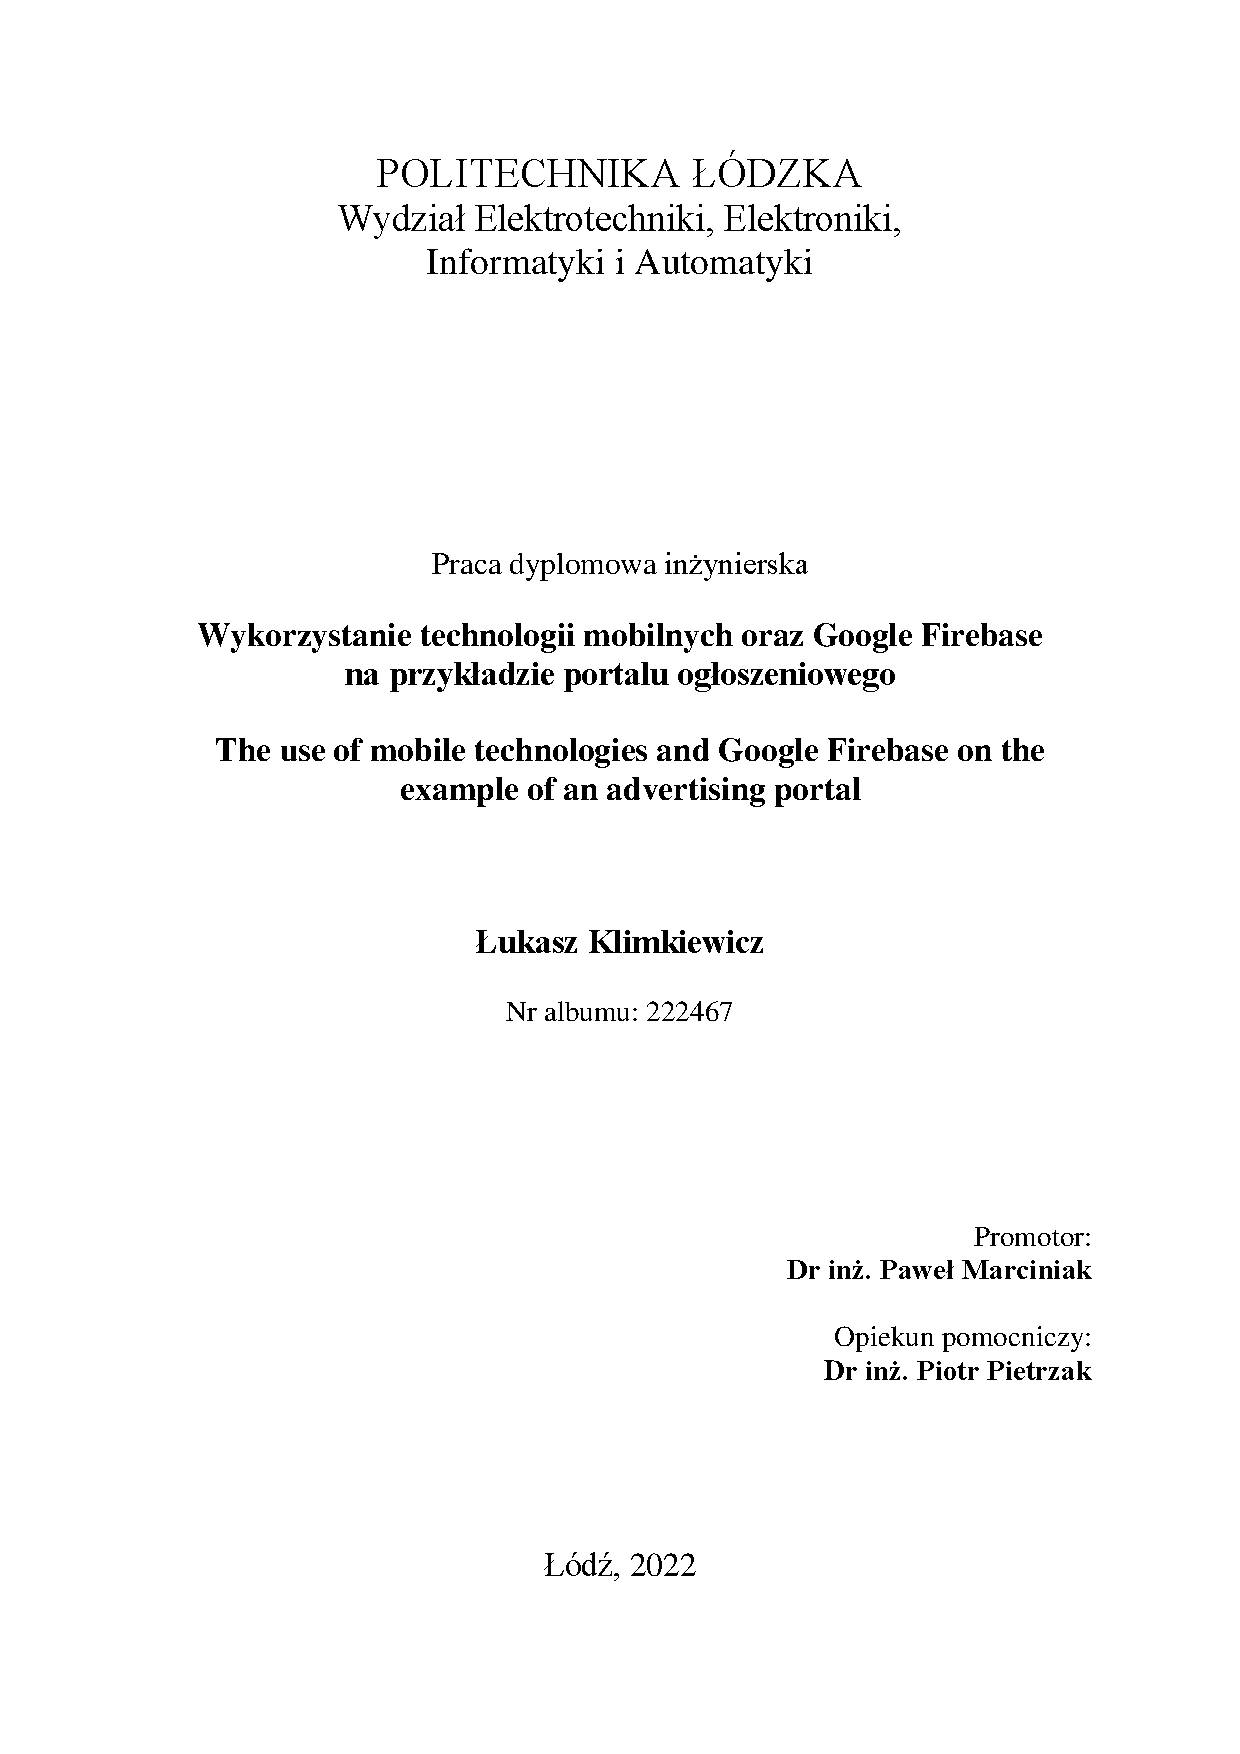
\includepdf[pages=-]{title_page.pdf}

% Numeruj od strony drugiej
\clearpage
\setcounter{page}{1}

% Abstrakt
% ==================== polski ==================== 
\section*{Streszczenie}
\vspace{1cm}

Celem niniejszej pracy dyplomowej było przedstawienie wykorzystania technologii mobilnych oraz platformy Google Firebase na przykładzie portalu pośredniczącego w świadczeniu usług. Miał on ułatwiać zamawianie ich przez klientów oraz oferowanie przez wykonawców.

Stworzone rozwiązanie umożliwia klientom dodawanie zleceń, które następnie są wysyłane do dopasowanych do nich wykonawców, mogących zgłaszać swoje oferty. Ze względu na dwie występujące w rozważanej domenie role zdecydowano się stworzyć również dwie aplikacje mobile. Jedna z nich przeznaczona jest dla usługobiorców, a druga dla usługodawców. Posiadają one chat zapewniający komunikację oraz system ocen i komentarzy, ułatwiający klientom podejmowanie właściwych wyborów. Przewidziano w nich również wsparcie dla pracy offline oraz dostosowanie interfejsu do ekranów tabletów. Platforma Firebase znacząco ułatwiła implementację powyższych elementów, lecz zauważono jej ograniczoną elastyczność.

% Celem niniejszej pracy dyplomowej było przedstawienie wykorzystania technologii mobilnych oraz platformy Google Firebase na przykładzie portalu pośredniczącego w świadczeniu usług. Miał on ułatwić łączenie klientów z wykonawcami oraz ich dalszą komunikację.

% Stworzone rozwiązanie polega na umożliwieniu klientom tworzenia zleceń, które następnie są wysyłane do odpowiednich wykonawców, mogących się do nich zgłaszać. Ze względu na dwie występujące w rozważanej domenie role zdecydowano się przygotować również dwie aplikacje mobilne. Jedna z nich jest przeznaczona dla usługobiorców, a druga dla usługodawców. Posiadają one chat, który zapewnia komunikację użytkowników oraz system ocen i komentarzy. Dzięki niemu klienci mogą wybierać wykonawcę usługi bazując na doświadczeniach wcześniejszych osób. W aplikacjach przewidziano również wsparcie dla pracy offline w ograniczonym zakresie oraz dostosowanie interfejsu do różnej wielkości ekranów. 


% Celem niniejszej pracy dyplomowej było przedstawienie wykorzystania technologii mobilnych oraz platformy Google Firebase na przykładzie portalu pośredniczącego w świadczeniu usług. Miał on umożliwiać klientom tworzenie zleceń, które następnie miały być wysyłane do odpowiednich wykonawców, mogących się do nich zgłosić. Na przygotowane rozwiązanie składają się dwie części: mobilne aplikacje klienckie oraz projekt Firebase.

% Ze względu na dwie występujące w rozważanej domenie role zdecydowano się stworzyć również dwie aplikacje mobilne. Jedna z nich jest przeznaczona dla usługobiorców, a druga dla usługodawców. Poza główną, opisaną funkcjonalnością, posiadają one chat, który zapewnia komunikację użytkowników oraz system ocen i komentarzy. Dzięki niemu klienci mogą wybierać wykonawcę usługi bazując na doświadczeniach wcześniejszych osób. W aplikacjach przewidziano również wsparcie dla pracy offline w ograniczonym zakresie oraz dostosowanie interfejsu do różnej wielkości ekranów. Dzięki temu wyglądają estetycznie zarówno na telefonach, jak i tabletach.

% Praca złożona jest z siedmiu rozdziałów poruszających następujące tematy. Pierwszy stanowi wstęp, w ramach którego przedstawiona została motywacja, cel i zakres pracy oraz założenia. Następy opisuje wykorzystane technologie, czyli wszystkie usługi, interfejsy, języki i środowiska, które odegrały rolę w procesie rozwoju projektu. Trzeci rozdział skupia się na bazie danych i porusza kwestię istniejącej w niej redundancji, a czwarty koncentruje na aplikacjach mobilnych. Została w nim dogłębnie opisana wykorzystana trójwarstwowa architektura oraz metoda współdzielenia kodu przez dwie tworzone aplikacje. W kolejnym rozdziale zawarto natomiast opis projektu Firebase i szczegółowo omówiono wszystkie jego części składowe, a w siódmym zostały obszernie omówione wszystkie zaimplementowane funkcjonalności. Ostatni rozdział stanowi podsumowanie całej pracy oraz proponuje możliwe drogi dalszego rozwoju aplikacji.

\vspace{1cm}
\noindent{\bf Słowa kluczowe:}
technologia mobilna, Android, Firebase, usługi
\clearpage

% ==================== angielski ==================== 
\section*{Abstract}
\vspace{1cm}

The aim of this thesis was to present the use of mobile technologies and the Google Firebase platform on the example of a service intermediary portal. It was supposed to facilitate ordering by customers and offering them by contractors.

The created solution allows customers to add orders, which are then sent to matching contractors, who can submit their offers. Due to the two roles occurring in the domain under consideration, it was decided to create also two mobile applications. One of them is intended for service recipients and the other for service providers. They have a chat feature for communication and a rating and commenting system to help customers make the right choices. They also provide support for offline work and adaptation of the interface to tablet screens. The Firebase platform has greatly facilitated the implementation of the above elements, but its limited flexibility has been noted.

% The aim of this thesis was to present the use of mobile technologies and the Google Firebase platform on the example of a service brokerage portal. It was supposed to facilitate connecting customers with contractors and their further communication.

% The created solution consists in enabling customers to create orders, which are then sent to the appropriate contractors, who may apply to them. Due to the two roles occurring in the domain under consideration, it was decided to also prepare two mobile applications. One of them is designed for service recipients and the other for service providers. They have a chat that provides communication between users and a rating and comment system. It allows customers to choose a service provider based on the experience of previous people. The applications also include support for limited offline work and adaptation of the interface to different screen sizes. 


% The aim of this thesis was to present the use of mobile technologies and the Google Firebase platform on the example of a service brokerage portal. It was supposed to enable customers to create orders, which were then sent to appropriate contractors, who could apply to them. The prepared solution consists of two parts: mobile client applications and Firebase project.

% Because of the two roles occurring in the considered domain, it was decided to create also two mobile applications. One of them is intended for service recipients and the other for service providers. Besides the main, described functionality, they have a chat, which provides communication between users, as well as a rating and comment system. It allows customers to choose a service provider based on the experience of previous customers. The applications also provide support for limited offline work and adaptation of the interface to different screen sizes. This makes them look aesthetically pleasing on both phones and tablets.

% The paper is composed of seven chapters covering the following topics. The first one is an introduction, which presents the motivation, goal, scope of the work and assumptions. The next describes the technologies used, that is all services, interfaces, languages and environments that played a role in the project development process. The third chapter focuses on the database and addresses the issue of redundancy in it, while the fourth focuses on mobile applications. It describes in depth the three-tier architecture used and the method of code sharing between the two applications being developed. The next chapter contains a description of the Firebase project and discusses all its components in detail, while the seventh provides an extensive description of all implemented functionalities. The last chapter is a summary of the whole work and suggests possible ways of further application development.

\vspace{1cm}
\noindent{\bf Keywords:} 
mobile technology, Android, Firebase, services
\clearpage


% Spis treści
\newpage
\section*{Spis treści} \
\vspace{2mm}
\tableofcontents\thispagestyle{fancy}
\clearpage

% Główna treść
\chapter{Wstęp}

Technologie mobilne cieszą się obecnie niewątpliwą popularnością. Telefony są wykorzystywane już nie tylko do komunikacji, lecz za sprawą różnorodnej funkcjonalności uczestniczą niemal we wszystkich dziedzinach życia. Według portalu Statista \cite{statista-mobiles-count} liczba aktualnie funkcjonujących urządzeń mobilnych wynosi 14,91 miliarda, a na najbliższe lata przewidywany jest dalszy wzrost ich liczebności. Lawinowo rośnie również liczba dostępnych aplikacji. Zgodnie z informacjami opublikowanymi przez ten sam portal \cite{statista-apps-count} w pierwszym kwartale 2021 roku w sklepie Google Play dostępnych było 3,48 miliona aplikacji, a w Apple App Store 2,22 miliona.

Sprostanie dużemu zapotrzebowaniu oraz wymaganiom gwałtownie zmieniającego się rynku wymaga szybkiego tworzenia i wprowadzania nowych aplikacji. Aby to ułatwić powstają i zyskują coraz większą popularność platformy dostarczające gotowych, kompleksowych rozwiązań w tym segmencie. Oferują szeroki wachlarz najczęściej wykorzystywanych usług, by deweloperzy nie byli zmuszeni do ich implementacji od podstaw, a mogli skupić na specyficznych dla aplikacji funkcjonalnościach. Wśród zapewnianych usług najczęściej znajdują się: baza danych, magazyn plików, system autoryzacji użytkowników, czy system notyfikacji push. Jedną z tego typu platform, cieszącą się powodzeniem, jest Google Firebase.

Zważając na dużą popularność aplikacji mobilnych oraz przydatne funkcjonalności oferowane przez platformę Google Firebase zdecydowano się na wykorzystanie oraz dokładniejsze zbadanie tych technologii.

% W niniejszej pracy postanowiono zbadać dokładniej możliwości oferowane przez technologie mobilne oraz Google Firebase.

\section{Cel oraz zakres pracy}

Celem pracy jest przedstawienie wykorzystania technologii mobilnych oraz Google Firebase na przykładzie rozwiązania umożliwiającego łatwe zamawiania przez klientów i oferowanie przez wykonawców różnego rodzaju usług. 

Z góry został założony podstawowy schemat działania systemu polegający na tym, że utworzone przez klientów zlecenia na wykonanie usług mają być wysyłane do dopasowanych pod nie wykonawców - decydujących, czy chcą się ich podjąć. Jest to o tyle istotne, że jest to model odwrotny w stosunku do powszechnie znanego modelu sprzedaży dóbr materialnych, w którym to sprzedający tworzą oferty, a kupujący decydują, czy je przyjąć. W przypadku usług tę odpowiedzialność - podjęcie decyzji - warto przenieść na stronę wykonawców, ponieważ po zapoznaniu się z ofertą to oni wiedzą najlepiej, czy posiadają odpowiednie umiejętności i narzędzia, i czy mogą wykonać usługę w żądanym terminie. 

% W przedstawionym mechanizmie klientom pozostawia się swobodę wyboru, ponieważ, jeżeli do zlecenia zgłosi się kilku wykonawców, to mogą oni wybrać tego, który najbardziej im odpowiada. Mogą też nie wybrać żadnego, jeśli mają takie życzenie. Aby ten mechanizm sprawnie działał w zakres pracy zdecydowano się włączyć system ocen i komentarzy. Dzięki niemu klienci szukający wykonawców do nowo stworzonych zleceń będą mogli bazować swoje decyzje na ocenach i komentarzach dodanych przez innych.

W przedstawionym mechanizmie klientowi pozostawia się swobodę wyboru wykonawcy - jeśli do zlecenia zgłosi się ich kilku, wybiera tego, który najbardziej mu odpowiada. Ma również prawno nie wybrać żadnego, jeżeli stwierdzi, że nie spełniają oni jego oczekiwań. W celu dopełnienia tej funkcjonalności w zakres pracy został włączony system ocen i komentarzy. Dzięki niemu usługodawcy wybierający wykonawców do nowo utworzonych zleceń będą mieli możliwość podjęcia decyzji na podstawie ocen i komentarzy pozostawionych przez innych.

W zakres pracy włącza się chat, który ma służyć za podstawowy kanał komunikacji pomiędzy klientami i wykonawcami. Za jego pomocą mogą być uzgadniane szczegóły realizacji usług, czy też ich koszty. O pojawieniu się nowej wiadomości lub zajściu innego istotnego zdarzenia użytkownicy powinni być informowani za pomocą powiadomień push. Postanowiono również zadbać o przystosowanie aplikacji do tabletów oraz umożliwić użytkownikom - w ograniczonym zakresie - pracę offline.

\section{Założenia}

% Dwie aplikacje
W tworzonym rozwiązaniu wyraźnie widoczne są dwie role: klienta oraz wykonawcy. Nie wykluczają się one wzajemnie, ponieważ jeden użytkownik może posiadać je obie. Z tego powodu jednym z pierwszych założeń, jakie należało poczynić była decyzja, czy temat zostanie zrealizowany w postaci jednej, uniwersalnej aplikacji mobilnej, czy też dwóch aplikacji dedykowanych, z których jedna będzie przeznaczona dla klientów, a druga dla wykonawców. Ostatecznie zdecydowano się na realizację dwóch aplikacji, ponieważ spodziewano się, że zdecydowaną większość użytkowników będą stanowili klienci, dla których obecność dodatkowych funkcjonalności związanych z wykonawcami będzie zbędna. Z ich punktu widzenia funkcjonalności te będą dodatkowo komplikowały interfejs, zwiększały rozmiar aplikacji i mogą doprowadzić do zniechęcenia części z nich.

% Zamykanie zleceń
Postanowiono też określić, jak długo tworzone przez klientów zlecenia mają być aktywne, czyli kiedy możliwość zgłaszania przez wykonawców swoich ofert ma być blokowana. Uznano, że siedem dni to maksymalny okres, ponieważ nawet rzadziej korzystający z aplikacji wykonawcy powinni zdążyć w tym czasie zapoznać się ze zleceniem. Ustalono także limit na liczbę wykonawców, którzy będą mogli zgłosić się w ramach jednego zlecenia - na liczbę ośmiu. Oznacza to, że po zgłoszeniu się przez ósmego wykonawcę zlecenie będzie zamykane. Czyniąc w ten sposób wspierano się artykułem psychologicznym, poruszającym tematykę efektu zbyt dużego wyboru \cite{choice-complexity}. Stwierdza się w nim, że posiadanie zbyt wielu alternatyw ostatecznie prowadzi do negatywnych konsekwencji, takich jak obniżona satysfakcja dokonanym wyborem. Z tego względu przyjęcie wspomnianego limitu powinno zapewnić zadowolenie klientów, przy jednoczesnym zachowaniu wyboru, który wciąż wydaję się wystarczający.

% Dopasowywanie zleceń
Jednym z kluczowych aspektów jest sposób, w jaki wykonawcy mają być dopasowywani do zleceń. Założono, że aby wykonawca mógł się zgłosić do realizacji zlecenia, musi realizować żądaną usługę oraz wymagane miejsce realizacji musi znajdować się wewnątrz obszaru jego działania. Wykonawcy muszą więc określać realizowane przez siebie usługi oraz wspomniany obszar. Postanowiono, że będzie on kołem, ponieważ umożliwia to jego proste definiowanie. Wystarczą do tego jedynie dwa parametry: centralna lokalizacja oraz promień.

% Lokalizacja
Przed przystąpieniem do implementacji ważne było poczynienie założenia co do obszaru na którym zakłada się, że będzie ona używana. Ma to oczywisty wpływ na język, ale wewnątrz aplikacji przewidziana została również możliwość wybierania lokalizacji przez użytkowników, która powinna zostać ograniczona do zadanego rejonu. Musi określić ją chociażby klient dla każdego nowo tworzonego zlecenia, aby mogło zostać wysłane do pobliskich wykonawców. Brak jakichkolwiek ograniczeń oznaczałby, że osoby mieszkające w pobliżu granicy mogłyby otrzymywać i zgłaszać się do zleceń osób z sąsiednich krajów, co nie zawsze mogłoby być pożądane, a nawet możliwe. Pojawiają się wówczas również problemy natury komunikacyjnej z powodu prawdopodobnie różnych języków narodowych. Z tych względów stwierdzono, że taka aplikacja powinna być ograniczona do jednego kraju, a konkretnie postanowiono ją przygotować dla Polski.

\pagebreak

% Optymalizacja kosztów
Ostatnim założeniem było zaimplementowanie wszystkich funkcjonalności, w miarę możliwości, w sposób zoptymalizowany pod względem kosztów. Większość usług wchodzących w skład platformy Firebase jest płatna, a obciążenia kosztami dokonuje się zwykle na podstawie intensywności ich wykorzystania. Zaniedbanie tego aspektu początkowo może nie stanowić problemu, lecz gdy aplikacja zyska popularność, to może ujawnić się brak jej skalowalności, objawiający się generowaniem wysokich kosztów. Z tego powodu należy przyjąć schematy przechowywania danych minimalizujące liczbę operacji, wykorzystać takie mechanizmy jak stronicowanie czy cachowanie, by temu zjawisku przeciwdziałać, a przynajmniej je ograniczać.

\chapter{Wykorzystane technologie i narzędzia}

% Firebase
\section{Platforma Firebase}
Platforma Firebase to zestaw narzędzi stworzony przez Google, który nie tylko umożliwia sprawne budowanie aplikacji, ale również ich monitorowanie i przyciąganie zainteresowania użytkowników. Składa się ona z obszernego zestawu współpracujących ze sobą usług, który trudno wykorzystać w pełni w jednym projekcie. W dalszej części zostały opisane te, które dla realizacji rozważanego tematu miały największe znaczenie. Więcej informacji na ich temat znajduje się w dokumentacji \cite{firebase-docs}.

Z platformy Firebase można korzystać w ramach dwóch planów: Spark oraz Blaze. Pierwszy jest darmowy i udostępnia bezpłatne, odnawiane co miesiąc limity. Jest wystarczający dla części aplikacji, jednak nie wszystkie funkcjonalności są w jego ramach dostępne. Wymusza to na wielu projektach przejście do planu drugiego. Zapewnia on te same darmowe limity, lecz po ich przekroczeniu automatycznie naliczane są koszty. Z uwagi na potrzebę wykorzystania usługi Firebase Functions, dostępnej jedynie w tym planie, musiał on zostać użyty.

\subsection{Firebase Authentication}
\label{technologie-authentication}
Firebase Authentication jest częścią platformy Firebase zapewniającą identyfikację i uwierzytelnianie użytkowników. 
Rozwiązanie to wspiera wiele metod logowania, zaczynając od klasycznego logowania za pomocą emaila i hasła, a kończąc na logowaniu społecznościowym. Istnieje możliwość wykorzystania numeru telefonu, portalu Google, Facebook, Twitter, Yahoo, Microsoft, Apple, Github czy też kont Google Play Games i Game Center. Każdemu zarejestrowanemu użytkownikowi przypisany zostaje unikalny i niezmienny ciąg znakowy zwany UID. Za jego pomocą jest on jednoznacznie identyfikowany. Firebase Authentication posiada również gotowe mechanizmy służące do weryfikacji adresów e-mail oraz numerów telefonu. 

\subsection{Firebase Firestore}
\label{technologie-firestore}

Firebase Firestore to nierelacyjna baza danych, która umożliwia łatwe przechowywanie danych, ich synchronizację oraz zadawanie zapytań. Została stworzona do bezpośredniej współpracy z aplikacjami klienckimi, które mogą na niej operować. 

Baza posiada wbudowaną funkcjonalność pracy offline, co jest szczególnie przydatne w przypadku urządzeń mobilnych, których połączenie z siecią nie jest stabilne. Gdy połączenia zabraknie, to dane odczytywane są z pamięci cache, a zapisy modyfikują jedynie lokalny obraz bazy, by ulec synchronizacji po przywróceniu połączenia.

Znaczącą zaletę Firestore stanowi wydajność, ponieważ usługa została zaprojektowana pod kątem jak największej skalowalności. Sprowadza się to do tego, że wraz ze zwiększaniem się ilości przechowywanych w niej danych, czas wykonywania zapytań nie rośnie. Jest on proporcjonalny jedynie do rozmiaru zbioru wynikowego.

Widocznym utrudnieniem użytkowania jest ograniczenie co do złożoności możliwych do stworzenia zapytań. Istnieje bowiem wiele reguł mówiących, że pewne operacje nie mogą być ze sobą łączone lub mogą, lecz warunkowo. Przykładem tego jest brak możliwości zawarcia w zapytaniu wielokrotnie operacji nierówności, chyba, że operacje te dotyczą tego samego pola.

Dla prostych zapytań baza Firestore automatycznie tworzy indeksy. Dla bardziej złożonych wymagane jest ich własnoręczne dodanie. W odróżnieniu bowiem od większości systemów bazodanowych, indeksy w Firestore nie przyspieszają zapytań, lecz w ogóle umożliwiają ich wykonanie.

\subsection{Firebase Cloud Storage}
\label{technologie-storage}

Firebase Cloud Storage to usługa zapewniająca przechowywanie obiektów plikowych. Typowo umieszczanymi w niej danymi są zdjęcia i filmy przesyłane przez użytkowników. Mogą być one porządkowane za pomocą struktury folderów, których zagnieżdżanie jest dozwolone. Każdy obiekt posiada metadane i nie ma przeszkód, by rozszerzyć je o dodatkowe, własne elementy.

Wśród oferowanych funkcjonalności znajduje się możliwość pauzowania oraz wznawiania transferów od momentu w którym zostały przerwane. Okazuje się to bardzo przydatne w przypadku urządzeń mobilnych, dla których przerwanie przesyłu jest często związane ze słabym połączeniem z siecią. Funkcja ta pozwala uniknąć straty czasu oraz zbędnego wykorzystania łącza na ponowne przesłanie tych samych danych. 

\subsection{Firebase Messaging}
Firebase Messaging to element platformy Firebase zapewniający sprawne wysyłanie wiadomości do urządzeń użytkowników. Przewiduje on istnienie dwóch rodzajów komunikatów. Pierwszym są wiadomości zawierające dowolne dane. Są one niezwykle elastyczne i możliwe do wykorzystania w wielu scenariuszach. Drugi rodzaj stanowią notyfikacje, których odebranie powoduje automatyczne pojawienie się powiadomienia. Jego zawartość oraz inne parametry określane są podczas wysyłania. Dostępne jest dla nich dostosowanie priorytetu, dźwięku powiadomienia, akcji kliknięcia, czy też czasu pojawienia się, co nie musi następować natychmiastowo.

Wszystkie urządzenia posiadają przypisane unikalne tokeny Firebase Cloud Messaging, w skrócie tokeny FCM. Są one wykorzystywane w celu adresowania do nich wiadomości. Inną metodą jest wysyłanie komunikatów w ramach tak zwanych tematów. Wówczas, aby urządzenie je dostawało, to musi odpowiedni temat zasubskrybować. Dostępne jest także zaawansowane określanie urządzeń docelowych na podstawie danych demograficznych i zachowań użytkowników.

% Wiadomości są komunikatami, które mogą zawierać dowolne informacje, a notyfikacje to powiadomienia push, pojawiające się na belce powiadomień. 

% Komunikaty mogą być wysyłane do poszczególnych urządzeń lub do wielu jednocześnie za pomocą tematów, które są przez nie subskrybowane.

% Możliwe jest również zaawansowane określanie urządzeń docelowych na podstawie danych demograficznych i zachowania użytkowników. Są one dostarczane natychmiastowo lub o zaplanowanym czasie. Możliwe jest określenie ich priorytetu, dźwięku powiadomienia i innych parametrów.

% Mogą być one tworzone i wysyłane przy pomocy wygodnego interfejsu graficznego dostępnego w konsoli Firebase. W przypadku potrzeby automatyzacji tego procesu lub wykorzystania zaawansowanych funkcjonalności konieczne jest wysyłanie ich z pomocą środowiska kontrolowanego, którym może być usługa Firebase Functions.

% Istnieje możliwość tworzenia i wysyłania notyfikacji przy pomocy wygodnego interfejsu graficznego dostępnego w konsoli Firebase. W przypadku potrzeby automatyzacji ich wysyłania lub wysłania wiadomości konieczne jest natomiast wykorzystanie środowiska kontrolowanego, którym najczęściej jest Firebase Functions.

\subsection{Firebase Functions}
\label{technologie-functions}

Firebase Functions to usługa, która umożliwia uruchamianie fragmentów kodu w pełni kontrolowanym środowisku, bez konieczności posiadania i zarządzania własnym serwerem. Jest to istotne, ponieważ urządzenia klienckie nie oferują poziomu bezpieczeństwa i niezawodności, który jest często wymagany.

% Możliwość uruchamiania kodu w kontrolowanym środowisku jest ważna, ponieważ występują ciągi operacji, które wymagają zachowania szczególnej spójności lub bezpieczeństwa. Aplikacje klienckie działające na telefonach użytkowników nie są takim środowiskiem, ponieważ w każdym momencie może zostać utracone połączenie z siecią lub wystąpić inny błąd, który przerwie być może krytyczną operację, doprowadzając tym samym do utraty spójności w systemie. 

Działanie usługi polega na umożliwieniu tworzenia funkcji w języku \mbox{JavaScript} lub \mbox{TypeScript} i zapewnieniu ich uruchomienia jedną z bardzo wielu dostępnych metod. Mogą być wywoływane bezpośrednio przez aplikacje klienckie, przez żądania http lub zostać zaplanowane i wywoływane zgodnie z harmonogramem. Przewidziane zostało również ich uruchamiane w odpowiedzi na zdarzenia występujące wewnątrz Firebase, takie jak rejestracja użytkownika, modyfikacja bazy danych, wysłanie pliku i wiele innych.

Kod źródłowy pisany jest na lokalnych maszynach, skąd następnie może zostać wdrożony w całości przy pomocy pojedynczego polecenia. Wdrożone funkcje są uruchamiane w całkowicie niezależnych od siebie kontenerach, zawierających wszystkie potrzebne elementy. Każda z nich w danym momencie może działać w kilku instancjach, których liczba dopasowuje się automatycznie do bieżącego obciążenia. Takie zachowanie funkcji zapewnia doskonałą skalowalność.

% Inną zaletą kodu backendowego jest to, że jest on całkowicie prywatny i użytkownicy aplikacji nie mają do niego w żaden sposób wglądu, w przeciwieństwie do kodu aplikacji klienckich, który również nie są przewidziany do oglądania przez użytkowników, ale może zostać poddany dekompilacji i procesowi inżynierii wstecznej przez osoby chcące to wykorzystać. 

% Kod backendowy jest również wykorzystywany w miejscach gdzie wymagane jest częste i szybkie wprowadzanie zmian. Zmodyfikowany kod backendowy będzie miał natychmiastowe zastosowanie do wszystkich użytkowników. Zaadaptowanie przez użytkowników nowszej wersji aplikacji klienckiej zajmuje natomiast znacznie więcej czasu.

\subsection{Firebase Security Rules}

Firebase Security Rules to elastyczny oraz kompletny język, który umożliwia definiowanie reguł ograniczających dostęp użytkowników do usług Firebase. Bezpośrednim celem tego działania jest zwiększenie bezpieczeństwa systemu. Podstawowa składnia języka jest zbliżona do JavaScript, lecz szczegóły różnią się w zależności od usługi, do opisywania której jest w danej chwili wykorzystywany. Obecnie wspiera on następujące usługi:

\begin{itemize}
    \item Cloud Storage
    \item Firestore
    \item Realtime Database
\end{itemize}

% Szczegóły tego języka różnią się dla każdej z wyżej wymienionych usług, lecz jego podstawowa składnia, która jest zbliżona do języka JavaScript, pozostaje podobna. 

Firebase dostarcza wygodne narzędzie wspomagające testowanie reguł nazwane Rules Playground, które jest dostępne za pomocą przeglądarki. Przy jego pomocy możliwe jest symulowanie wykonywania szerokiej gamy operacji w zdefiniowanym kontekście, a w odpowiedzi uzyskanie informacji o tym, która reguła daną operację zaakceptowała lub odrzuciła.


% \subsection{Firebase Pub/Sub}
% Firebase Pub/Sub to usługa zapewniająca globalną magistralę wiadomości, która doskonale się skaluje. Jak nazwa wskazuję umożliwia ona pracę w modelu producent-subskrybent. Producenci komunikują się z subskrybentami poprzez wysyłanie asynchronicznych komunikatów zamiast bezpośredniego wywoływania funkcji. Komunikaty te mogą zawierać dodatkowe informacje na temat jakiegoś zdarzenia, które mogą być wykorzystane przez konsumentów. Są wysyłane poprzez nazwane kanały, zwane tematami. Jednym z możliwych producentów jest Google Scheduler, czyli usługa umożliwiająca wykonywanie akcji, takich jak wysyłanie komunikatów Pub/Sub o zaplanowanym czasie, w tym w sposób periodyczny. Aby zaplanować więc wykonanie jakiegoś zadania należy takie wiadomości zasubskrybować i w odpowiedzi na nie wykonać odpowiednią akcję.

\subsection{Firebase Emulators Suite}
Firebase Emulators Suite to zestaw  narzędzi dla twórców oprogramowania umożliwiający uruchomienie emulatorów usług Firebase na lokalnej maszynie, które działają identycznie jak ich wersje produkcyjne. Zestaw ten składa się z siedmiu emulatorów składowych, umożliwiających emulację następujących usług:

\begin{multicols}{2}
    \begin{itemize}
        \item Auth
        \item Firestore
        \item Cloud Storage
        \item Functions
        \item Realtime Databse
        \item Hosting
        \item Pub/Sub
    \end{itemize}
\end{multicols}

Po odpowiednim skonfigurowaniu możliwa jest komunikacja aplikacji z wymienionymi wyżej emulatorami, działającymi na lokalnej maszynie, zamiast środowisku produkcyjnym. Jeżeli część z nich nie zostanie skonfigurowana lub wykorzystywane są usługi, których emulacja nie jest zapewniona, to aplikacja nadal będzie komunikowała się z ich wersjami produkcyjnymi.

Firebase Emulators Suite, poza standardową emulacją, oferuje również dodatkowe funkcjonalności. Pierwszą z nich jest możliwość zapisywania oraz przywracania wcześniej zapisanego stanu poprzez funkcje eksportu i importu. Jest to szczególnie przydatne w kontekście reprodukcji błędów oraz pracy przy trudno odtwarzalnych stanach. Kolejną funkcjonalnością jest szybkie reagowanie na wprowadzane zmiany. Wdrożenie ich do środowiska produkcyjnego zajmuje bowiem do kilku minut. Firebase Emulators Suite jest w stanie natomiast automatycznie wykryć zmiany i natychmiastowo je zaaplikować. Umożliwia to szybkie prototypowanie i testowanie.


% \subsection{FirebaseUI}
% Przedstawienie narzędzia i jak zostało wykorzystane.

%Google maps
\section{Platforma Google Maps}
Platforma Google Maps to zestaw interfejsów API (ang. Application Programming Interface) oraz bibliotek SDK (ang. Software Development Kit) umożliwiających deweloperom umieszczanie w aplikacjach map oraz pobieranie różnych informacji z nimi związanych. Wykorzystanie tego typu narzędzia było konieczne, ponieważ zarówno zlecenia, jak i wykonawcy są powiązani z lokalizacjami, które należy przetwarzać i w jakiś sposób wizualizować. 

Poza rozwiązaniem oferowanym przez Google rozważane były również inne możliwości, takie jak MapBox. Istotne w kontekście projektu różnice pomiędzy nimi okazały się jednak na tyle niewielkie, że wybrano Google, ze względu na wykorzystywaną już platformę Google Firebase i chęć uniknięcia komplikacji projektu poprzez włączanie do niego kolejnych dostawców usług.

Na Platformę Google Maps składają się trzy produkty: Maps, Routes oraz Places. Dwa z nich zostały wykorzystane przy realizacji rozważanego tematu i dokładniej opisane poniżej. 

%W celu uzyskania bardziej szczegółowych informacji należy odwołać się do dokumentacji Google Maps Platform \cite{maps-docs}.

\subsection{Maps}
Jest to produkt, który umożliwia umieszczanie w aplikacjach mobilnych i webowych dynamicznych oraz statycznych map, a także dostosowywanie ich w szerokim zakresie. W jego ramach dostępna jest funkcja Street View, dająca możliwość zobaczenia wybranych części świata z poziomu ulicy oraz interfejs pozwalający na pobieranie danych związanych z wysokością. Został wykorzystany w projekcie ze względu na łatwe osadzenia map wewnątrz aplikacji mobilnych, co można osiągnąć przy pomocy gotowych bibliotek.

\subsection{Places}
Jest to część platformy Google Maps, która daje dostęp do wielu informacji dotyczących miejsc, takich jak godziny otwarcia, oceny odwiedzających czy zdjęcia. Agreguje interfejsy umożliwiające wyszukiwanie miejsc, autouzupełnianie ich nazw podczas pisania, czy określanie stref czasowych. Zapewnia też geolokalizację, czyli funkcjonalność określania przybliżonego położenia urządzenia na podstawie pobliskich stacji bazowych i sieci Wi-Fi. Istotną funkcjonalnością, o której należy wspomnieć, jest również geokodowanie, czyli możliwość konwersji adresów na współrzędne geograficzne i odwrotnie. Geokodowanie oraz autouzupełnianie nazw lokalizacji to funkcjonalności, które przy realizacji rozważanego tematu okazały się przydatne.

%Języki
\section{Języki programowania}

Język programowania to podstawowe narzędzie wykorzystywane do rozwoju aplikacji. Wybór języka lub ich zestawu rzutuje na szereg innych elementów. Należało więc dokonać go bardzo rozważnie, biorąc pod uwagę wiele aspektów. Podstawowe z nich to funkcjonalności oferowane przez dany język, zapewnione wsparcie, ilość dostępnych bibliotek czy też popularność, za którą stoi wielkość społeczności, która w razie wystąpienia problemów może pomóc. Rozważań dokonano w kontekście projektu, gdyż każdy ma swoje własne wymagania.

\subsection{Kotlin}
Do rozwoju aplikacji mobilnych dla systemu Android wybrany został język Kotlin. Jest to statycznie typowany język działający na maszynie wirtualnej Javy, rozwijany głównie przez firmę JetBrains. W 2017 roku na konferencji Google I/O został ogłoszony oficjalnym językiem programowania dla platformy Android. Z tego powodu wsparcie dla niego w przyszłości będzie zapewne coraz bardziej rosnąć, na rzecz wcześniej wykorzystywanej Javy. Minusem jest to, że jest on od niej znacznie młodszy, więc trzeba się liczyć z mniejszą społecznością i liczbą materiałów. 

Język Kotlin jest w pełni interoperacyjny z Javą, co oznacza, że można w nim swobodnie korzystać z bibliotek języka Java, a wnosi dodatkowo wiele udogodnień. Jednym z nich jest wprowadzenie \enquote{null safety}, czyli braku możliwości przypisania do zmiennej typu referencyjnego wartości null, jeżeli w jawny sposób nie wyrażono na to zgody. Eliminuje to w dużym stopniu niebezpieczeństwo związane z tego typu wskaźnikami. Wprowadza również funkcje rozszerzeń, które umożliwiają dodawanie nowych funkcjonalności do już gotowych komponentów, korutyny, które znacznie upraszczają programowanie współbieżne i wiele więcej.

\subsection{TypeScript}
TypeScript to silnie typowany język bazujący na JavaScript i transpilowany do niego, który został wybrany do tworzenia kodu funkcji w ramach Firebase Functions. Został stworzony przez Microsoft w 2012 roku. Jedyną alternatywę dla niego stanowi czysty JavaScript, ponieważ usługa Firebase Functions nie wspiera innych języków. Bezpośrednim powodem wybrania właśnie TypeScript, jest to, że jest do tego zastosowania zalecany przez Google.

Główną cechą wyróżniającą TypeScript na tle JavaScript jest statyczne typowanie. Poza nim wprowadza moduły oraz przestrzenie nazw, jako skuteczny sposób modularyzacji kodu. Dodaje interfejsy oraz typy wyliczeniowe. Zmiany te powodują, że zdecydowana większa ilość błędów może zostać wykryta już na etapie kompilacji. Jeżeli natomiast chodzi o wady, to należy zauważyć, że TypeScript, dodając etap transpilacji, wprowadza dodatkowy narzut czasowy, nieistniejący dla jedynie interpretowanego języka JavaScript.

Porównując popularność obu języków można się oprzeć na ankiecie przeprowadzonej wśród deweloperów przez Stack Overflow w 2021 roku \cite{stackoverflow-ankieta}. Wynika z niej, że JavaScript jest zdecydowanie najpopularniejszą technologią, wykorzystywaną przez 64.96\% ankietowanych, a korzystanie z TypeScript zadeklarowało jedynie 30.19\%. Większa społeczność jest zaletą języka JavaScript, a wynika ona z długiej historii tego języka i wielu projektów w nim rozpoczętych. Z tej samej ankiety wynika jednak, że TypeScript jest bardziej uwielbianym językiem i w rankingu technologi, których deweloperzy chcieliby używać, plasuję się przed JavaScriptem.

% Środowiska
\section{Środowisko programistyczne}
Wybór odpowiedniego środowiska stanowi istotny punkt procesu rozwoju oprogramowania. Nowoczesne narzędzia znacznie go usprawniają poprzez automatyczne uzupełnianie kodu, czy też sugerowanie błędów już podczas jego pisania. Pozwala to zaoszczędzić wiele czasu i wysiłku. Środowisko powinno być jednak jak najbardziej dopasowane do potrzeb projektu, by zapewnić wsparcie, którego on potrzebuje. Z tego powodu zostało to dokładnie przemyślane.

\subsection{Android Studio}
Android studio jest to IDE (ang. Integrated Development Environment), które zostało wybrane do rozwoju aplikacji mobilnych. Jest oficjalnym środowiskiem programistycznym dla platformy Android i w związku z tym oferuje szeroki wachlarz funkcjonalności. Umożliwia tworzenie aplikacji w języku Kotlin, Java oraz C++, a inteligentny edytor kodu zapewnia trafne podpowiedzi. Odznacza się obecnością wizualnego edytora układów, który pozwala na tworzenie nawet skomplikowanych interfejsów użytkownika przy pomocy metod \mbox{WYSIWYG} (ang. What You See Is What You Get). Ponadto posiada emulator, który daje możliwość testowanie aplikacji na urządzeniach o różnych rozmiarach i wersjach oprogramowania oraz narzędzia służące do profilowania w czasie rzeczywistym, uwzględniające wykorzystanie pamięci, procesora i ruch sieciowy. Dużą zaletą jest również zaawansowany system budowania: Gradle. Pozwala on tworzyć kilka wersji jednej aplikacji, a w wyniku budowania przygotowuje gotowy plik o rozszerzeniu apk, będący gotowym do dostarczenia użytkownikom.

% Do celów konfiguracji wykorzystuje on język domenowy, którym może być Groovy lub Kotlin. Daje możliwość tworzenia kilku wersji aplikacji przy pomocy wariantów budowania (ang. build variants) oraz smaków produktów (ang. product flavors). Rezultatem budowania jest plik o rozszerzeniu apk, będący gotowym do dostarczenia użytkownikom.


\subsection{Visual Studio Code}
Visual Studio Code to edytor kodu źródłowego stworzony przez Microsoft. Zgodnie z badaniem przeprowadzonym w 2021 roku przez Stack Overflow \cite{stackoverflow-ankieta} było to wówczas najczęściej wykorzystywane przez deweloperów środowisko. Zostało wybrane do rozwoju projektu Firebase ze względu na swoją prostotę i możliwość rozbudowy. Dostępnych jest bowiem dla niego wiele rozszerzeń, pozwalających dostosować funkcjonalności do potrzeb. Wśród tych wykorzystanych można wymienić rozszerzenie wspierające tworzenie reguł Firebase Security Rules poprzez kolorowanie składni i podpowiedzi, czy też zapewniające wsparcie dla języka TypeScript. Środowisko posiada debugger i umożliwia wygodną pracę z system kontroli wersji GIT.

\chapter{Architektura}

\begin{figure}[ht]
  \centering
  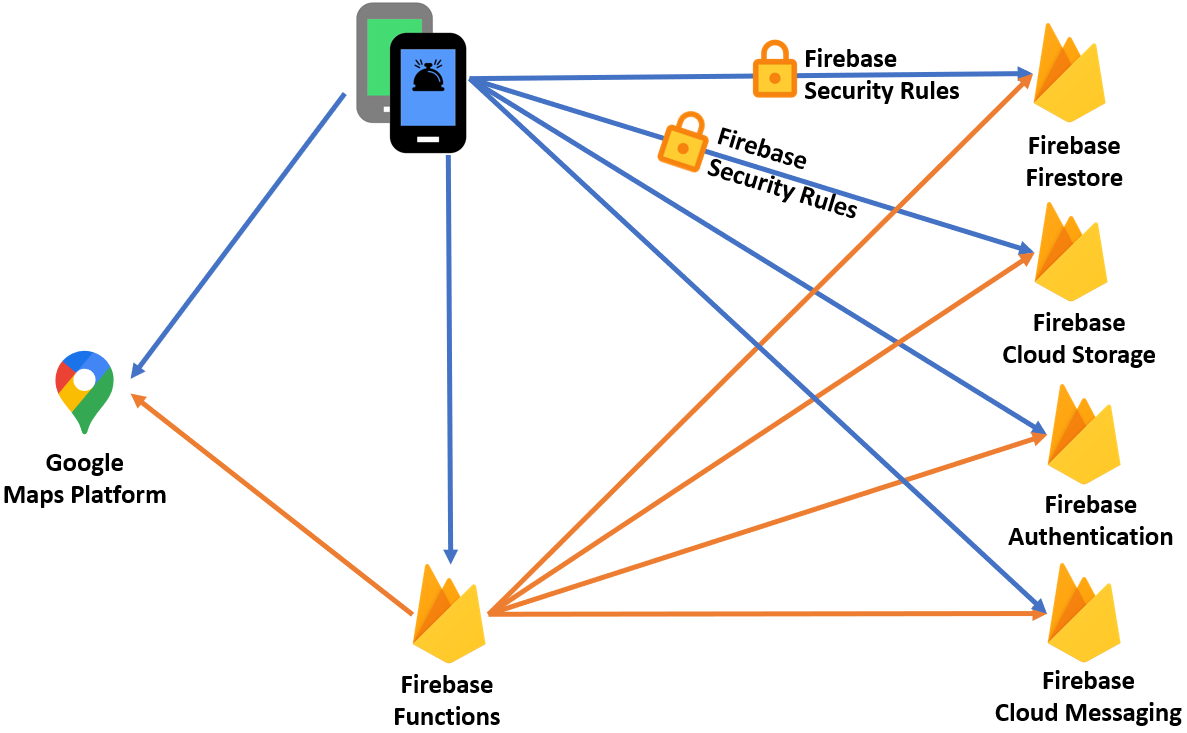
\includegraphics[width=\linewidth]{images/architecture.png}
  \caption{Schemat architektury systemu}
  \label{fig:architecture}
\end{figure}

Na rysunku \ref{fig:architecture} przedstawiona została wysokopoziomowa architektura stworzonego systemu. Składa się na nią siedem komponentów połączonych relacjami zależności.

Najważniejszym elementem z punktu widzenia użytkowników są aplikacje mobilne. W celu zapewnienia swojej funkcjonalności korzystają one ze wszystkich innych komponentów. Dostęp do bazy danych Firestore oraz magazynu plików Cloud Storage jest jednak ograniczony przez reguły bezpieczeństwa, by uniemożliwić wykonywanie przez użytkowników niepożądanych operacji.

Usługa Firebase Functions to drugi ważny komponent. Odgrywa rolę backendu. Aplikacje klienckie delegują do niej wykonywanie części operacji. Zajmuje się ona również synchronizacją pomiędzy różnymi częściami systemu. Jest to środowisko kontrolowane, więc żadne ograniczenia dostępu nie są potrzebne.

Implementacja przedstawionego systemu została podzielona na dwie równolegle rozwijane części. Pierwszą z nich stanowią aplikacje klienckie, a drugą projekt Firebase, który obejmuje funkcje Firebase Functions oraz reguły bezpieczeństwa Firebase Security Rules.

% Implementacja przedstawionego systemu została podzielona na dwie równolegle rozwijane części. Pierwszą z nich stanowią aplikacje klienckie, opisane w rozdziale \ref{part:applications}, a drugą projekt Firebase, przedstawiony w rozdziale \ref{part:firebase}. Włączają się w niego funkcje Firebase Functions oraz reguły Firebase security Rules. W osobnym rozdziale została opisana także baza danych, ponieważ obie części z niej korzystają.
% Baza danych
\chapter{Baza danych}

W projekcie została wykorzystana baza danych Firebase Firestore, która jest rozwiązaniem typu NoSQL, opierającym się na dokumentach. Przez Firebase oferowana jest również baza Realtime Database, jednak po dokładnym rozważeniu różnic pomiędzy nimi zdecydowano się ją odrzucić. Głównym przeznaczeniem Realtime Database jest bowiem, jak sugeruje nazwa, przechowywanie i praca na szybko zmieniających się danych, dla których zapewnia małe opóźnienia i wydajną synchronizację pomiędzy klientami. Może to mieć duże znaczenie w przypadku gier, lecz dla tworzonych aplikacji nie jest to krytyczny aspekt. Baza Firestore oferuje za to bardziej intuicyjny sposób przechowywania danych, szybsze oraz bardziej złożone zapytania oraz lepszą skalowalność.

Sposób przechowywania danych przez bazę Firestore w znaczny sposób odbiega od sposobu robienia tego w klasycznych bazach relacyjnych. Zapisuje ona wszystkie dane w dokumentach, które są pogrupowane w kolekcje. Poza istnieniem wysokopoziomowych kolekcji możliwe jest również tworzenie podkolekcji wewnątrz dokumentów, przez co można osiągnąć zagnieżdżoną strukturę.

% Zarówno dokumenty jak i kolekcje posiadają identyfikatory.

\section{Model bazy danych}

Firestore, jako nierelacyjna baza danych, nie posiada modelu, czy schematu, a przynajmniej nie jest on narzucony przez samą bazę. Objawia się to tym, że pozwala ona na przechowywanie wewnątrz jednej kolekcji dokumentów posiadających kompletnie różne zestawy pól, a nawet dynamiczną zmianę ich typów. Mimo wszystko, baza wymaga pewnego uporządkowania i podczas jej projektowania wykształcił się pewien schemat, który zostanie opisany.

Na rysunku \ref{fig:baza-kolekcje} przedstawione zostały wykorzystane kolekcje. Jak widać przewidzianych zostało osiem wysokopoziomowych kolekcji oraz trzy podkolekcje. Należy je rozumieć w taki sposób, że każdy jeden dokument wewnątrz kolekcji \code{offers} posiada własną kolekcję \code{messages}, a każdy jeden dokument wewnątrz kolekcji \code{clients} oraz \code{experts} posiada własną kolekcję \code{tokens}. 

\begin{figure}[ht]
  \centering
  \includegraphics[width=\linewidth]{images/db_collections.png}
  \caption{Diagram stworzonych w bazie kolekcji}
  \label{fig:baza-kolekcje}
\end{figure}

\vspace{\baselineskip}

% \noindent Znaczenie stworzonych kolekcji jest następujące:
\noindent W każdej kolekcji przechowywane są dokumenty reprezentujące inne obiekty, które są następujące:
\begin{itemize}
    \item \textbf{\code{services}} - usługi, które klienci mogą zlecać, a wykonawcy wykonywać;
    \item \textbf{\code{categories}} - kategorie, na które zostały podzielone usługi;
    \item \textbf{\code{clients}} - klienci;
    \item \textbf{\code{experts}} - wykonawcy;
    \item \textbf{\code{jobs}} - zlecenia tworzone przez klientów;
    \item \textbf{\code{offers}} - oferty zgłaszane do zleceń;
    \item \textbf{\code{ratings}} - oceny dawane wykonawcom przez klientów;
    \item \textbf{\code{matches}} - informacje o wykonawcach dopasowanych do zleceń;
    \item \textbf{\code{tokens}} - tokeny FCM, wykorzystywane do wysyłania notyfikacji;
    \item \textbf{\code{messages}} - wiadomości wysyłane przez chat.
\end{itemize}

\vspace{\baselineskip}

Dokładna zawartość dokumentów znajdujących się w wymienionych kolekcjach została przedstawiona na rysunku \ref{fig:baza-dokumenty}. Wraz z każdym znajdującym się w nich polem wypisane zostały typy, które może ono przyjmować. Dla oznaczenia, że dane pole może być nieobecne wprowadzono sztuczny typ \code{absent}, który to oznacza.

\begin{figure}[ht!]
  \centering
  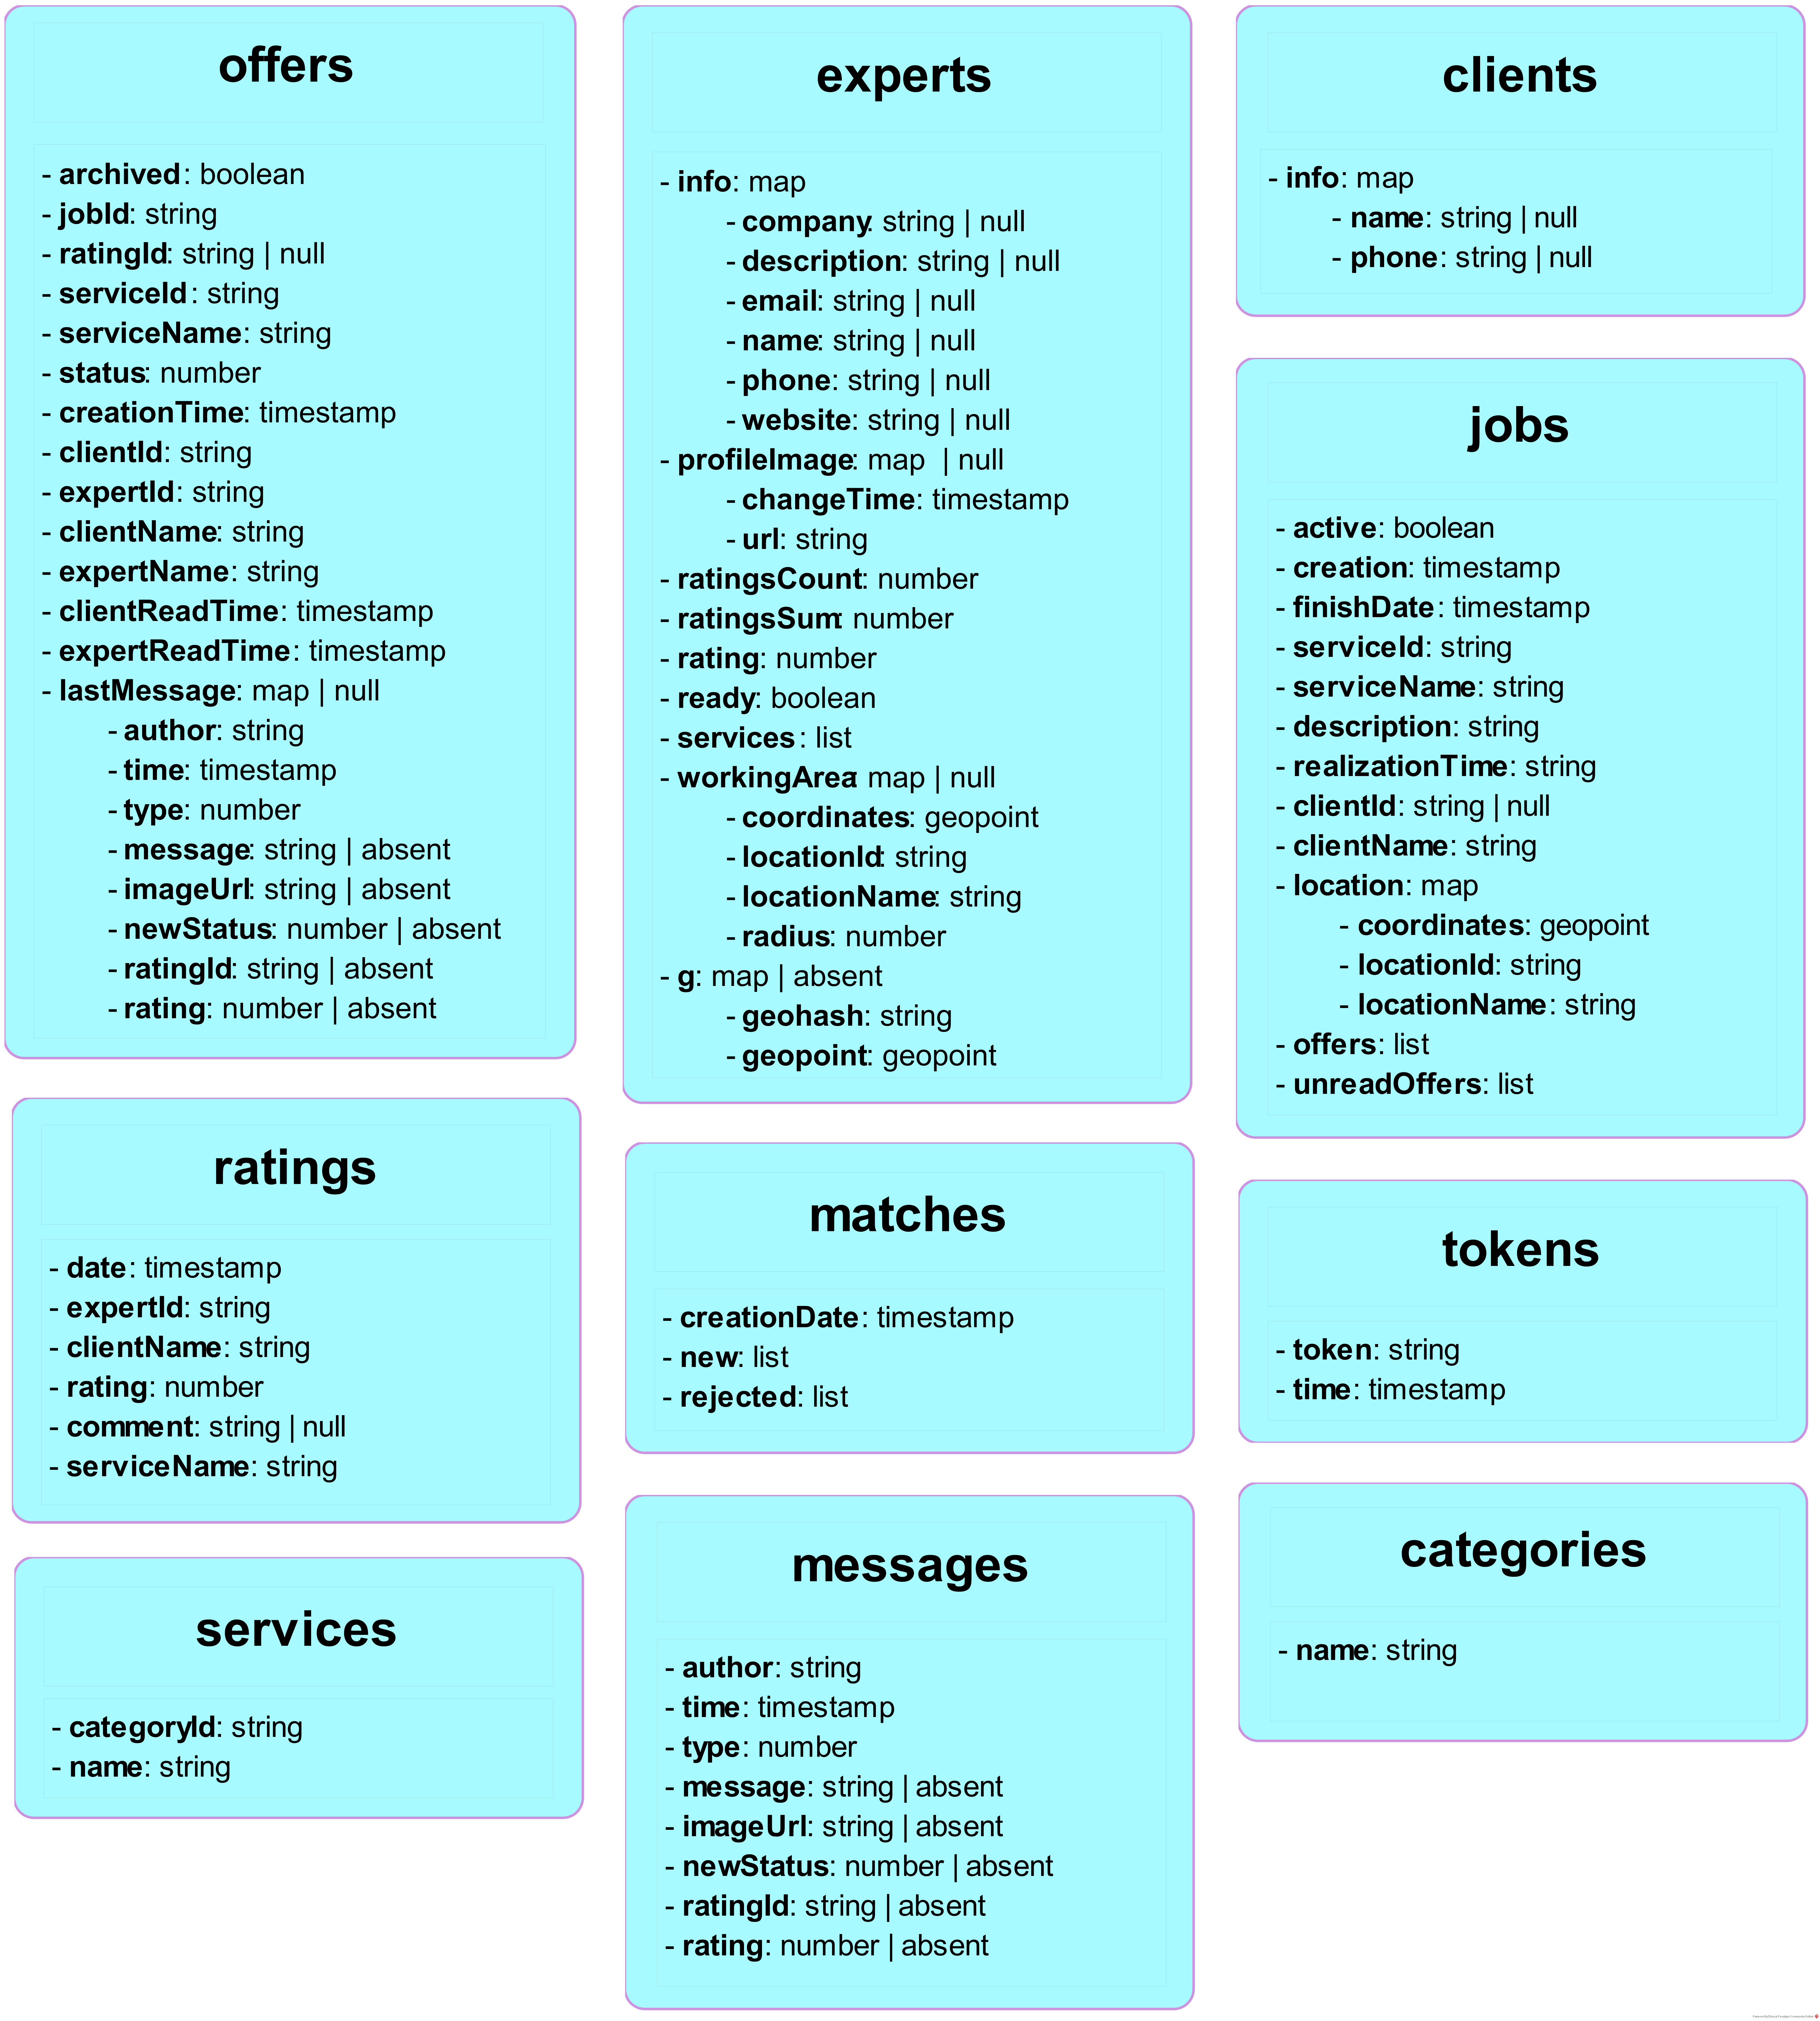
\includegraphics[width=\linewidth]{images/db_documents.png}
  \caption{Schematy dokumentów w poszczególnych kolekcji bazy danych}
  \label{fig:baza-dokumenty}
\end{figure}

\pagebreak

Łączenie pomiędzy dokumentami dokonuje się poprzez umieszczenie w jednym z nich identyfikatora innego. Przykładem tego jest znajdujące się wewnątrz dokumentów w kolekcji \code{services} pole \code{categoryId}, które zawiera identyfikator dokumentu z kolekcji \code{categories} i w ten sposób stworzona zostaje jednokierunkowa relacja jeden do wielu pomiędzy usługami, a ich kategoriami. Nadając nazwy pól przyjęto konwencję, że każde pole, którego nazwa posiada sufiks \code{Id} jest referencją do innego dokumentu.

\section{Redundancja}

\noindent Redundancja to nadmiarowość w stosunku do tego, co konieczne. W przypadku baz danych jej prostym przykładem jest przechowywanie tych samych informacji w kilku miejscach. Zwykle dąży się do usunięcia redundancji, czyli normalizacji, ponieważ niepotrzebnie zwiększa rozmiar bazy i naraża ją na brak spójności. Mimo wszystko można ją zaobserwować na przedstawionym schemacie bazy w następujących miejscach:

% \noindent Na szczególną uwagę zasługuję istniejąca w bazie w kilku miejscach redundancja. Jest 

\vspace{0.5\baselineskip}

\begin{itemize}
    \item Dokumenty w kolekcjach \code{offers} oraz \code{jobs} posiadają pole \code{serviceName} zawierające nazwę usługi, chociaż wartość ta może zostać uzyskana poprzez wykorzystanie referencji \code{serviceId}, znajdującej się w tych dokumentach i odczytanie pola \code{name} z odpowiedniego dokumentu w kolekcji \code{services}.
    \item Dokumenty w kolekcji \code{offers} posiadają pole \code{expertName} zawierające imię i nazwisko wykonawcy, chociaż wartość ta może zostać uzyskana poprzez wykorzystanie referencji \code{expertId}, znajdującej się w tych dokumentach i odczytanie pola \code{info.name} z odpowiedniego dokumentu w kolekcji \code{experts}.
    \item Dokumenty wewnątrz kolekcji \code{offers} oraz \code{jobs} posiadają pole \code{clientName} zawierające imię i nazwisko klienta, chociaż wartość ta może zostać uzyskana poprzez wykorzystanie referencji \code{clientId}, znajdującej się w tych dokumentach i odczytanie pola \code{info.name} z odpowiedniego dokumentu w kolekcji \code{clients}.
\end{itemize}

Wskazana redundancja została wprowadzona celowo, a jej przeznaczeniem jest uniknięcie konieczności podążania referencjami i odczytywania dodatkowych dokumentów. Generowałoby to dodatkowe koszty, ponieważ Firebase nalicza je między innymi względem liczby odczytanych dokumentów. Dodatkowo przyczyniłoby się do większego ruchu sieciowego, który na urządzeniach mobilnych należy ograniczać z powodu zużycia baterii i możliwych ograniczeń transferu.

Aby zrozumieć, dlaczego redundancja została wprowadzona akurat w tych miejscach należy odwołać się do interfejsu użytkownika, a konkretnie ekranów przedstawionych na rysunku \ref{fig:ekrany-redundancja}. Są to główne ekrany obu aplikacji, więc będą często wyświetlane i wszystkie trzy zawierają listy, które mogą być potencjalnie bardzo długie. Są więc ekranami w przypadku których szczególnie warto zadbać o minimalizację liczby odczytywanych dokumentów. 

\begin{figure}[ht]
  \captionsetup[subfigure]{justification=centering}
  \centering
  \begin{subfigure}{0.32\textwidth}
    \centering
    \fbox{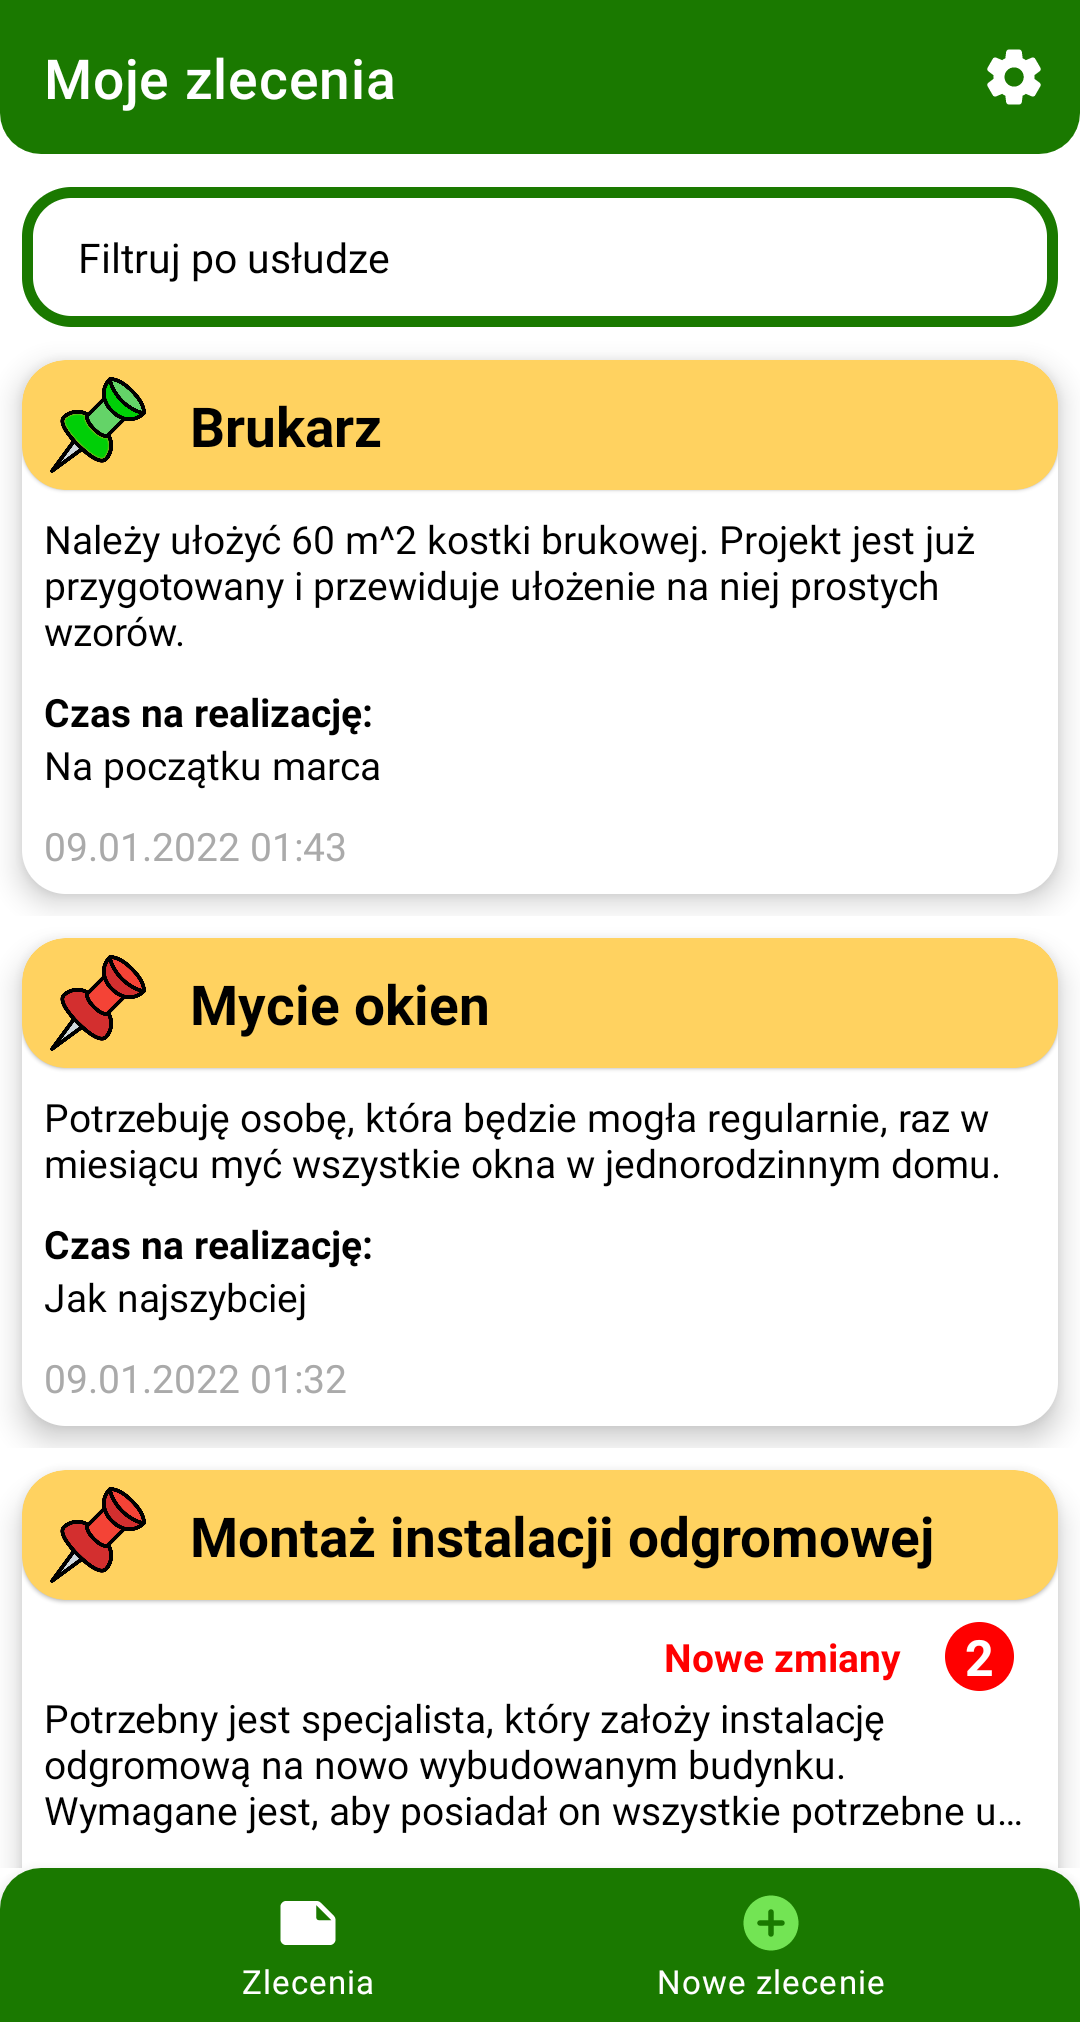
\includegraphics[width=0.97\linewidth]{screens/client_jobs.png}}
    \caption{Ekran dodanych zleceń\\(aplikacja dla klientów)}
  \end{subfigure}
  \begin{subfigure}{0.32\textwidth}
    \centering
    \fbox{
\includegraphics[width=0.95\linewidth]{screens/expert_jobs.png}}
    \caption{Ekran dostępnych zleceń\\(aplikacja dla wykonawców)}
  \end{subfigure}
  \begin{subfigure}{0.32\textwidth}
    \centering
    \fbox{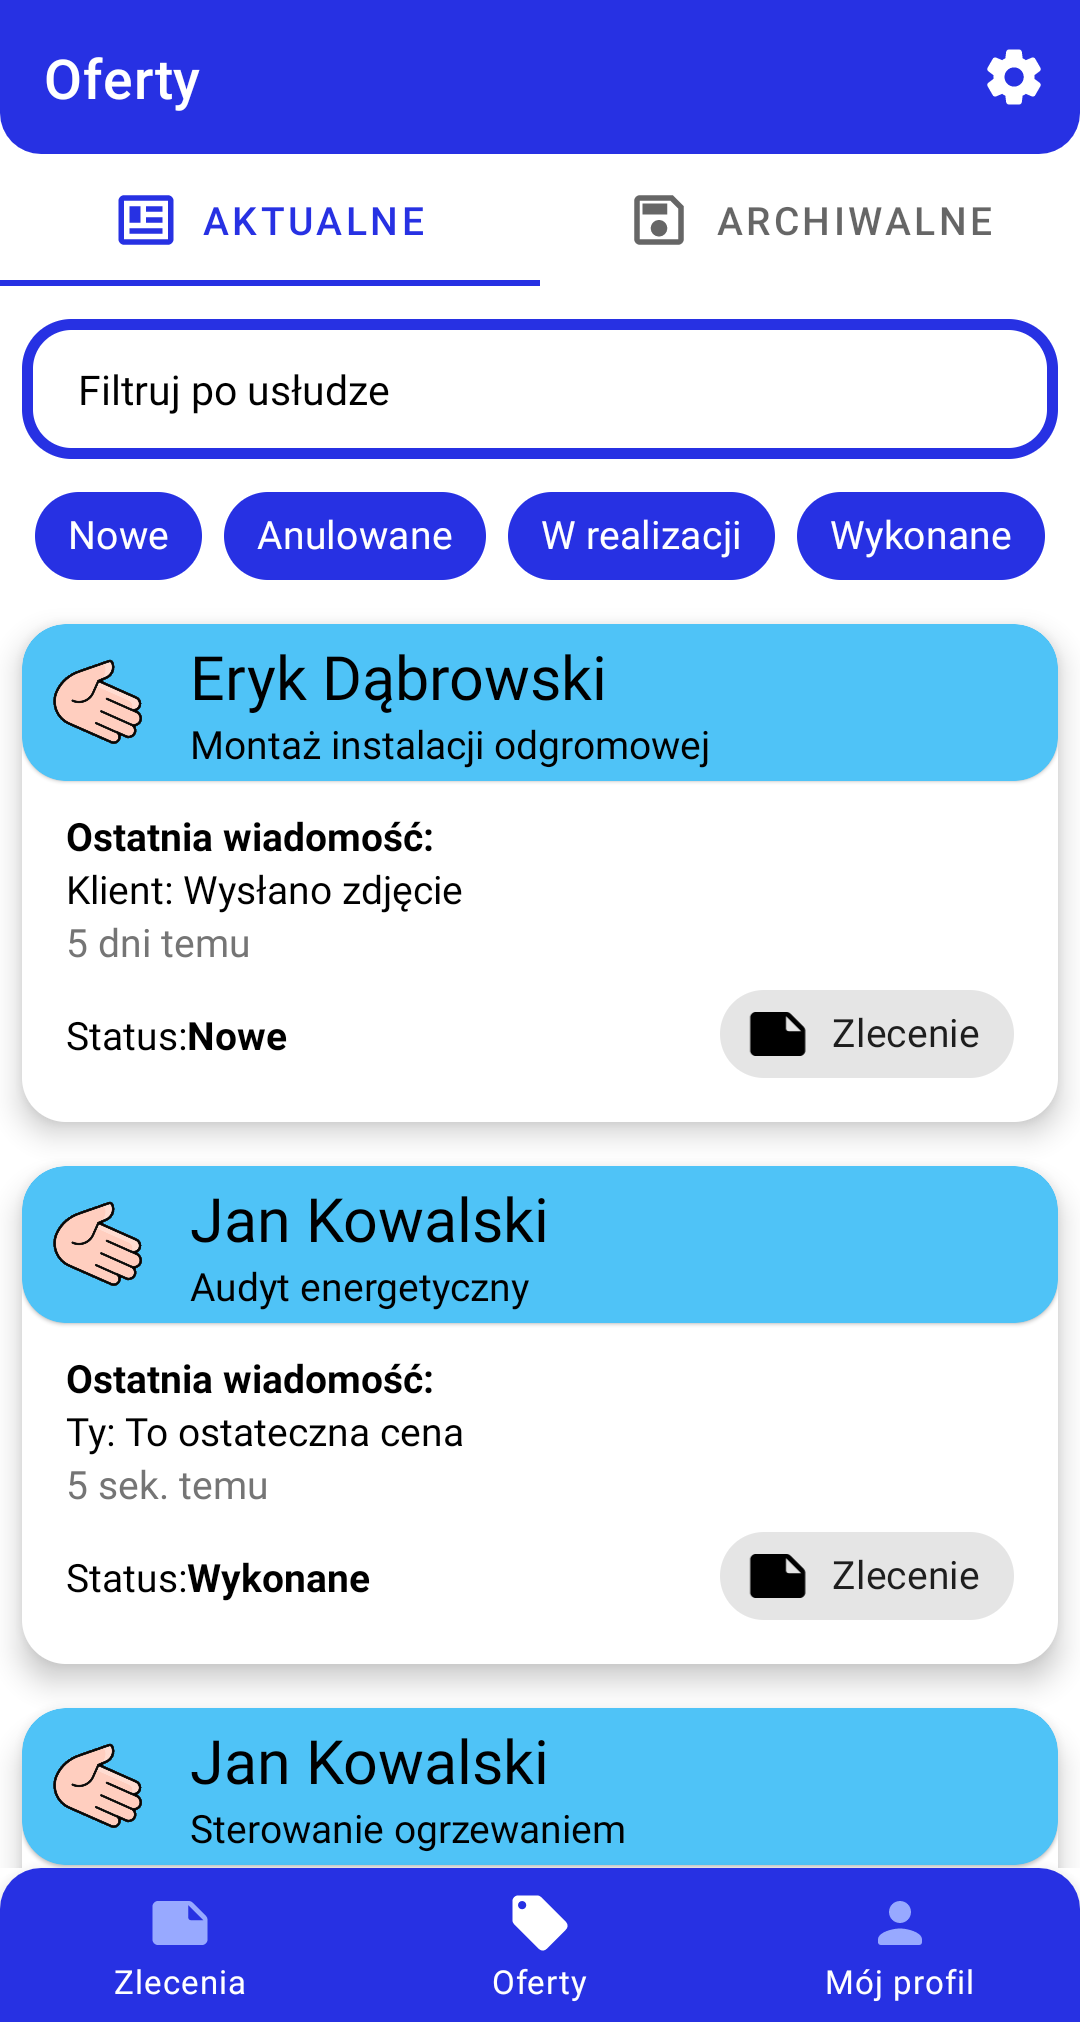
\includegraphics[width=0.95\linewidth]{screens/expert_offers_no_swap.png}}
    \caption{Ekran złożonych ofert\\(aplikacja dla wykonawców)}
  \end{subfigure}
  \caption{Ekrany mające wpływ na wprowadzoną w bazie redundancję}
  \label{fig:ekrany-redundancja}
\end{figure}

W przypadku ekranu (a), przedstawionego na rysunku \ref{fig:ekrany-redundancja}, lista zawiera zlecenia, wraz z nazwami usług, których dotyczą. Dzięki temu, że dokumenty zleceń zawierają nazwy usług, to dla każdego elementu listy wystarczy odczytać tylko jeden dokument. W przeciwnym wypadku konieczne byłoby zaangażowanie dodatkowej kolekcji i zwiększenie liczby odczytywanych dokumentów dwukrotnie.

W przypadku ekranu (b) dla każdego zlecenia, oprócz nazwy usługi, wyświetlana jest również nazwa klienta, więc w tym przypadku redundancja pozwala zmniejszyć liczbę odczytywanych dokumentów nawet trzykrotnie.

Dla ekranu (c) redundancja również zmniejsza liczbę odczytywanych dokumentów trzykrotnie, ponieważ umożliwia uniknięcie odczytywania dokumentów z kolekcji \code{experts}, by dostać nazwisko wykonawcy i kolekcji \code{services}, by dostać nazwę usługi.

% Należy zauważyć, że aby wprowadzanie redundancji było sensowne to częstotliwość odczytywania rozważanych informacji musi być znacząco większa od częstotliwości ich modyfikacji, ponieważ konieczne jest utrzymywanie spójności danych, poprzez aktualizowanie wartości we wszystkich miejsach na raz, zamiast jednego

\section{Zapytania związane z lokalizacjami}

Baza danych, wśród innych informacji, przechowuje lokalizacje związane ze zleceniami oraz wykonawcami. Jest to bardzo proste z powodu dostępnego w Firestore typu geopoint, zawierającego w sobie zarówno szerokość, jak i wysokość geograficzną. Okazuje się jednak, że pomimo obecności tego typu, baza nie wspiera wykonywania żadnych specyficznych dla lokalizacji kwerend. 
Podczas implementacji okazało się jednak konieczne zwrócenie wszystkich dokumentów zawierających lokalizację, znajdującą się w zadanym maksymalnym promieniu od pewnego, centralnego punktu. Operacja ta została zwizualizowana na rysunku \ref{fig:query}.

\begin{figure}[ht]
  \centering
  \fbox{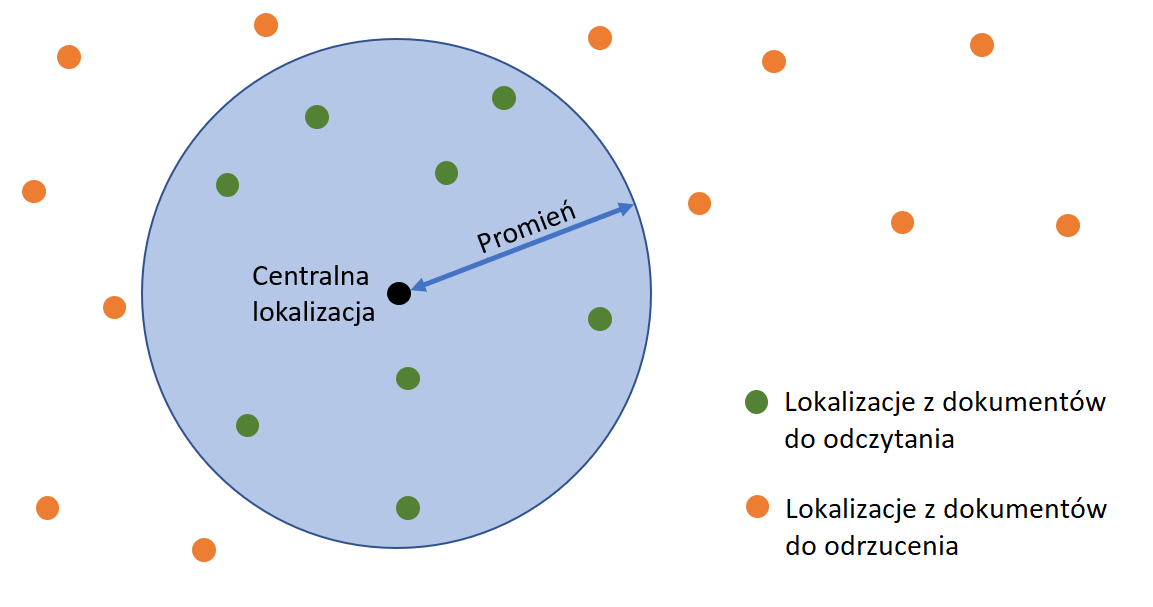
\includegraphics[width=0.7\linewidth]{images/query_visualization.png}}
  \caption{Wizualizacja potrzebnej operacji związanej z lokalizacją}
  \label{fig:query}
\end{figure}

Jak zostało wspomniane, Firestore nie posiada żadnych mechanizmów ułatwiających wykonanie tego typu zapytania. Wciąż istnieją jednak pewne drogi umożliwiające rozwiązanie powstałego problemu.

Najbardziej naiwnym rozwiązaniem jest pobieranie wszystkich dokumentów jeden po drugim, obliczanie dla każdego z nich odległości do centralnej lokalizacji i zaliczanie do zbioru wynikowego, jeżeli jest ona odpowiednio mała. Ma to jednak ogromną wadę w postaci odczytu dużej liczby dokumentów i w związku z tym generowaniem wysokich kosztów. Z tego powodu metoda ta została szybko odrzucona.

Rozsądnym rozwiązaniem byłoby określenie ramki okalającej (ang. bounding box), w której muszą znajdować się wszystkie lokalizacje z potrzebnych do odczytania dokumentów. Mogłyby z niej zostać odczytane poprzez dokonanie filtracji jednocześnie po odpowiednim zakresie szerokości i wysokości geograficznych. Problem w tym, że Firestore nie pozwala na wykonanie takiej operacji w jednym zapytaniu. W jednej kwerendzie należałoby dokonać filtracji po zakresie szerokości, a w drugiej po zakresie wysokości i przeprowadzić ręczne połączenie ich wyników operacją iloczynu mnogościowego. Podczas niej zostanie jednak odrzuconych wiele dokumentów, co oznacza, że ich odczyty spowodowały niepotrzebne koszty.

% Rozsądnym podejściem byłoby zwrócenie nieco większego zbioru dokumentów poprzez dokonanie filtracji jednocześnie po odpowiednim zakresie szerokości i wysokości geograficznych, a następnie odrzucenie z niego niechcianych elementów. Problem w tym, że Firestore nie pozwala wykonania takiej operacji w jednym zapytaniu. Konieczne byłoby wykonanie dwóch kwerend, a następnie samodzielne połączenie ich wyniku. Również ta metoda wiąże się z dużą liczbą niepotrzebnie odczytywanych dokumentów.

% Najlepszym rozwiązaniem okazuje się wykorzystanie geohashy, które umożliwiają wydajne wykonywanie tego typu operacji. Są one ciągami znaków, w których zakodowana jest zarówno szerokość, jak i wysokość geograficzna. Mają ciekawą własność polegającą na tym, że im wspólny prefiks dwóch z nich jest dłuższy, tym lokalizacje, które reprezentują, znajdują się bliżej siebie. Geohashe zostały dodane do dokumentów z kolekcji \code{experts}. Aby zapewnić możliwość prostego ich wykorzystania, została użyta biblioteka geofirestore. Zapewnia ona wyszukiwanie dokumentów na podstawie położenia geograficznego i dostarcza potrzebną operację.

Najlepszym rozwiązaniem okazuje się wykorzystanie geohashy, które umożliwiają wydajne wyszukiwanie na podstawie lokalizacji. Są one ciągami znaków, w których zakodowana jest zarówno szerokość, jak i wysokość geograficzna. Mają ciekawą właściwość polegającą na tym, że im wspólny prefiks dwóch z nich jest dłuższy, tym lokalizacje, które reprezentują, znajdują się bliżej siebie. Aby zapewnić możliwość ich prostego wykorzystania, została użyta biblioteka geofirestore. Zapewnia ona wyszukiwanie dokumentów na podstawie położenia geograficznego i dostarcza potrzebną operację.

% \begin{figure}[ht]
%   \centering
%   \includegraphics[width=0.5\linewidth]{images/geohash_fancy.png}
%   \caption{Wizualizacja logiki stojącej za algorytmem geohashy \cite{geohash-fancy}}
%   \label{fig:geohash}
% \end{figure}
% Frontend
\chapter{Aplikacje mobilne}
\label{part:applications}

% Brak przecinka przed zamiast
Oparcie rozwiązania o Firebase pozwoliło znacznie uprościć część backendową, która sprowadza się jedynie do opisanego w kolejnym rozdziale projektu Firebase. Dodało to jednak wiele odpowiedzialności ciążących na stronie klienckiej. Dodatkowo decyzja o stworzeniu dwóch aplikacji mobilnych zamiast jednej przyczynia się do dalszej jej komplikacji. Z wymienionych powodów opracowanie aplikacji mobilnych stanowiło dominującą część całego projektu i zastosowane wewnątrz nich rozwiązania wymagały głębokiego przemyślenia.

% Brak przecinka przed zamiast
% Oparcie projektu o Firebase pozwala znacznie uprościć lub wręcz usunąć część backendową, lecz dodaje więcej odpowiedzialności ciążących na stronie klienckiej. Należy równocześnie mieć na uwadze wcześniejsze założenie, co do stworzenia dwóch aplikacji mobilnych zamiast jednej. Z wymienionych powodów implementacja części klienckiej stanowi dominującą część całego projektu i dlatego zastosowane wewnątrz niej rozwiązania wymagają głębokiego przemyślenia.

\section{Architektura}

Odpowiednio dobrana architektura umożliwia płynny rozwój aplikacji, nawet, przy bardzo dużej i ciągle rosnącej bazie kodu. Jest to również najważniejszy element wpływający na solidność oraz możliwość testowania.

Jedną z główny cech, jaką dobra architektura powinna się charakteryzować, jest jasne i precyzyjne określenie odpowiedzialności posiadanych przez poszczególne części programu. Sam podział aplikacji na jak najbardziej niezależne sekcje jest sugerowany przez regułę projektowania zwaną skrótowo SoC (ang. Separation of Concerns). Zgodnie z nią każda z nich powinna zajmować się innym problemem, pracować z innymi informacjami.

Architekturą, która doskonale spełnia wymienione wymagania, jest trójwarstwowa architektura rekomendowana przez Google dla aplikacji mobilnych. Składają się na nią warstwy prezentacji, domenowa oraz danych, z których każda pełni inne funkcje. Zostały one przedstawione na rysunku \ref{fig:ca-warstwy}.

\begin{figure}[ht]
  \centering
  
\includegraphics[width=0.8\linewidth]{images/arch_layers.png}
  \caption{Schemat warstw aplikacji}
  \label{fig:ca-warstwy}
\end{figure}

Warstwa prezentacji jest odpowiedzialna za przekazywanie informacji użytkownikowi, aktualizowanie ich, jeżeli ulegają zmianie oraz przechwytywanie podejmowanych przez niego akcji, takich jak kliknięcia czy przesunięcia po ekranie.

Warstwa danych zapewnia dostęp do informacji przechowywanych w różnego rodzaju trwałych magazynach. Zawiera w sobie logikę dotyczącą sposobu pobierania, tworzenia, modyfikowania oraz usuwania różnych obiektów.

Celem warstwy domenowej jest przechowywanie logiki biznesowej. Jest ona zawarta w postaci tak zwanych przypadków użycia. Każdy z nich odpowiada za inny scenariusz. Przykładowe przypadki użycia, które zostały stworzone to dodanie zlecenia, wysłanie wiadomości, pobranie dostępnych zleceń czy wylogowanie. Ich obecność umożliwia zamknięcie skomplikowanej logiki oraz wielokrotne użycie. Warstwa ta zawiera również klasy określające obiekty domenowe, czyli te najistotniejsze, takie jak zlecenie, wiadomość, wykonawca czy klient.

Zgodnie ze wskazówkami dotyczącymi architektury, znajdującymi się w dokumentacji platformy Android, obecność warstwy domenowej nie jest zawsze konieczna. W przypadku, gdy aspekt ponownego wykorzystania nie jest kluczowy oraz logika biznesowa jest prosta, to może ona prowadzić do powstania większej ilości kodu, bez wprowadzenia dodatkowych korzyści. Biorąc jednak pod uwagę, że tworzone będą dwie aplikacje, które z pewnością będą współdzieliły część logiki biznesowej stwierdzono, że wielokrotne użycie jest istotną kwestią i zdecydowano się tę warstwę wykorzystać.

% Na warstwę domenową składają się dwa typy elementów: modele domenowe oraz przypadki użycia. Modele domenowe to klasy reprezentujące pojęcia występująca w dziedzinie rozważanego problemu, np. zlecenie, oferta, wykonawca, klient czy wiadomość. Przypadki użycia są to natomiast operacje związane z tą dziedzina, np. dodanie zlecenia, akceptacja oferty, wysłanie wiadomości, pobranie dostępnych zleceń czy wylogowanie.

% Bardzo ważny jest kierunek zależności istniejących pomiędzy tymi warstwami. Zarówno warstwa prezentacji jak i warstwa danych jest zależna od warstwy domenowej. Umożliwia to skupienie się na dziedzinie aplikacji, która stanowi jej rdzeń. Ten kierunek umożliwia również dokonywanie zmian w warstwie prezentacji i warstwie danych bez większego wpływu na warstwy pozostałe.

% Aby zrozumieć przydatność przypadków użycia należy wiedzieć, że wykonywane przez nie operacje mogą być dość skomplikowane. Przykładem jest przypadek użycia polegający na pobraniu informacji o zleceniu z punktu widzenia aktualnie zalogowanego wykonawcy. W pierwszej kolejności, korzystając z warstwy danych, pobiera on identyfikator aktualnego użytkownika. Następnie pobiera podstawowe informacje o zleceniu i korzystając z wcześniej pobranego identyfikatora użytkownika, pobiera status zlecenia. Ostatecznie łączy te wyniki do postaci pojedynczego obiektu domenowego, który zwraca. W ten sposób udaje się zamknąć wewnątrz niego dużą złożoność, a warstwa prezentacji, która go wywołuje jest świadoma jedynie parametrów oraz zwracanej przez niego wartości, co jest ważne tym bardziej, że jeden przypadek może być wykorzystywany w kilku miejscach.

% Wykorzystanie przypadków użycia usprawniło również obsługę błędów. Operacje wykonywane w ich ramach mogą bowiem często zakończyć się błędem. Czasami niepowodzenie jednej z operacji cząstkowych oznacza niepowodzenia całego przypadku użycia, a czasem nie. 

% Owszem, zdarza się, że przypadki użycia bezpośrednio odpowiadają metodom znajdującym się w warstwie danych, jak ma to miejsce w przypadku dodawania oceny, gdzie na przypadek użycia składa się tylko jedno wywołanie.

\section{Warstwa prezentacji}
\label{wzorzec-mvvm}

W ramach warstwy prezentacji wykorzystany został wzorzec MVVM (ang. Model-View-ViewModel), który umożliwia czyste i jasne oddzielenie kwestii związanych z interfejsem użytkownika od warstwy domenowej. Stosowanie go jest wspierane przez platformę Android poprzez dostarczanie gotowych komponentów, które to ułatwiają. Dostępna jest między innymi klasa ViewModel, która umożliwia zachowanie w niej stanu aplikacji podczas zmian konfiguracji, takich jak obroty urządzenia.

Tak jak sugeruje nazwa, na wzorzec MVVM składają się komponenty: Model, View oraz ViewModel. Zostały one przedstawione wraz z relacjami pomiędzy sobą na rysunku \ref{fig:mvvm}.

\begin{figure}[ht!]
  \centering
  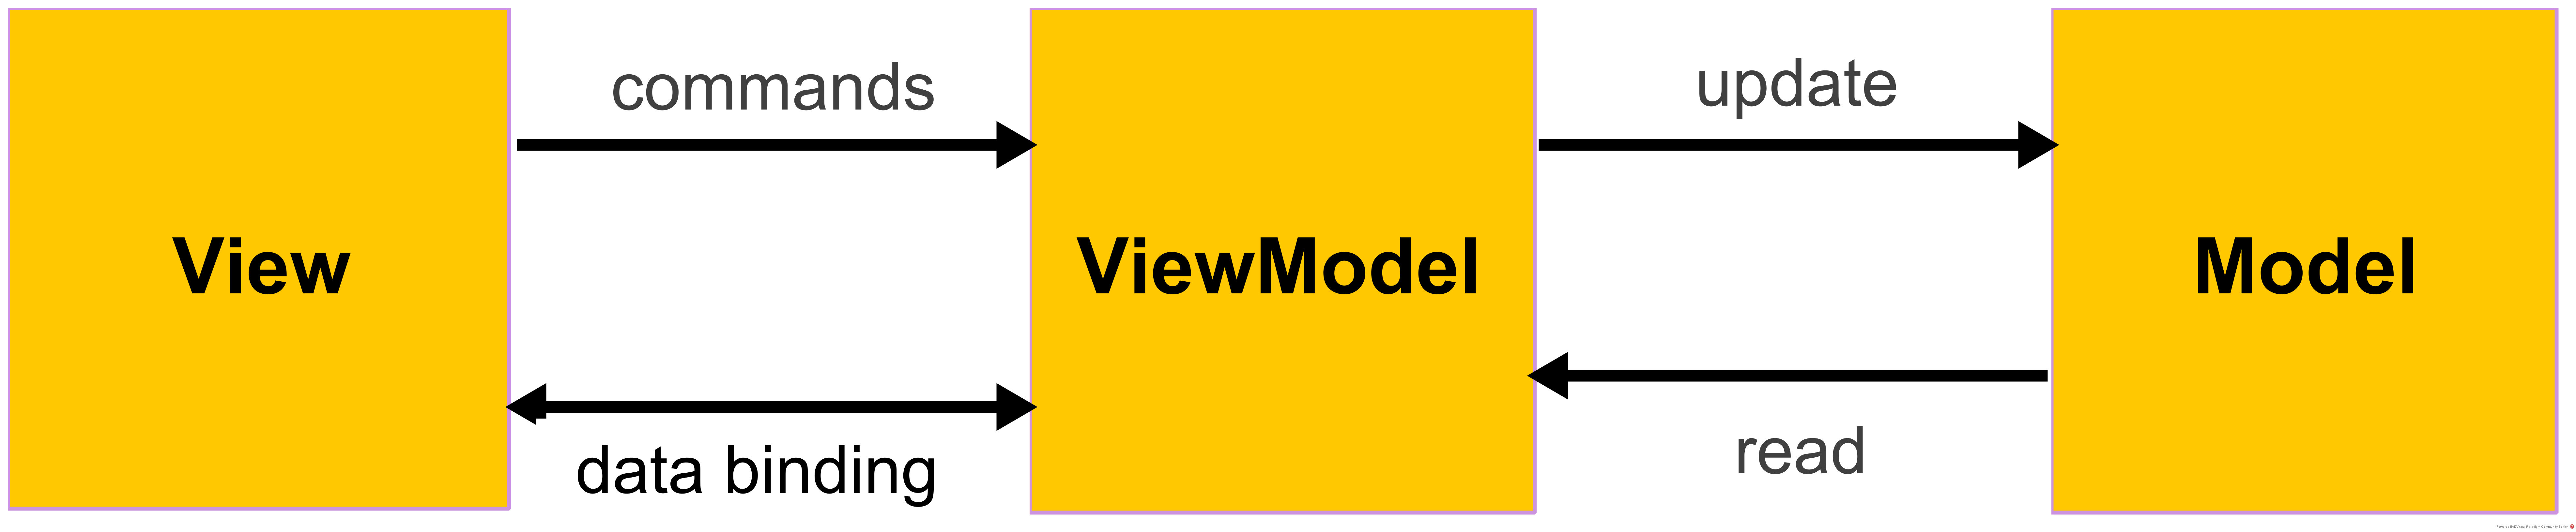
\includegraphics[width=\linewidth]{images/mvvm_general.png}
  \caption{Schemat komponentów wzorca MVVM i ich relacji}
  \label{fig:mvvm}
\end{figure}

View jest widokiem, czyli tym co widzi użytkownik oraz z czym wchodzi w interakcję. W przygotowanym rozwiązaniu wszystkimi widokami są fragmenty, które stanowią reużywalną część interfejsu użytkownika, więc doskonale się do tego nadają. Komponent model odnosi się z kolei do modelu biznesowego i oznacza całą warstwę domenową, na którą składają się przypadki użycia i modele domenowe. Ostatnim komponentem jest ViewModel, który pełni ważna funkcję polegającą na połączeniu dwóch pozostałych. W ten sposób umożliwia ich niezależny rozwój. Ponadto przechowuje stan.

Interakcja komponentu ViewModel z modelem biznesowym sprowadza się do wykonywania przypadków użycia, za pomocą których model może zostać zmodyfikowany lub mogą zostać z niego odczytane dane.
Widok nie może robić tego bezpośrednio, więc jeśli potrzebuje wejść w interakcję z modelem, to jedynie za pośrednictwem ViewModel.

Pomiędzy komponentami View oraz ViewModel wykorzystywana jest technika zwana data binding, która w ogólnym znaczeniu polega na zapewnieniu synchronizacji ze sobą dwóch źródeł danych. Dzięki niej każda zmiana stanu komponentu ViewModel może zostać natychmiastowo odzwierciedlona w widoku. Możliwe są także wiązania dwukierunkowe, zapewniające synchronizację w obie strony. Korzystanie z tej techniki jest proste, z uwagi na dostępną w ramach Android Jetpack biblioteki, która ją wspiera.

%Wykonuje przypadki użycia z warstwy domenowej i po ewentualnym przetworzeniu udostępnia ich wyniki widokowi, by mógł je wyświetlić.



% Komunikacja ViewModel z View zachodzi poprzez mechanizm subskrypcji udostępniany przez obiekty LiveData, będące częścią platformy Android. Gdy widok zasupskrybuje taką wartość, to będzie powiadamiany o wszystkich jej późniejszych zmianach.

%W celu usprawnienia komunikacji pomiędzy View oraz ViewModel wykorzystana została biblioteka Data Binding

% \begin{figure}[ht!]
%   \centering
%   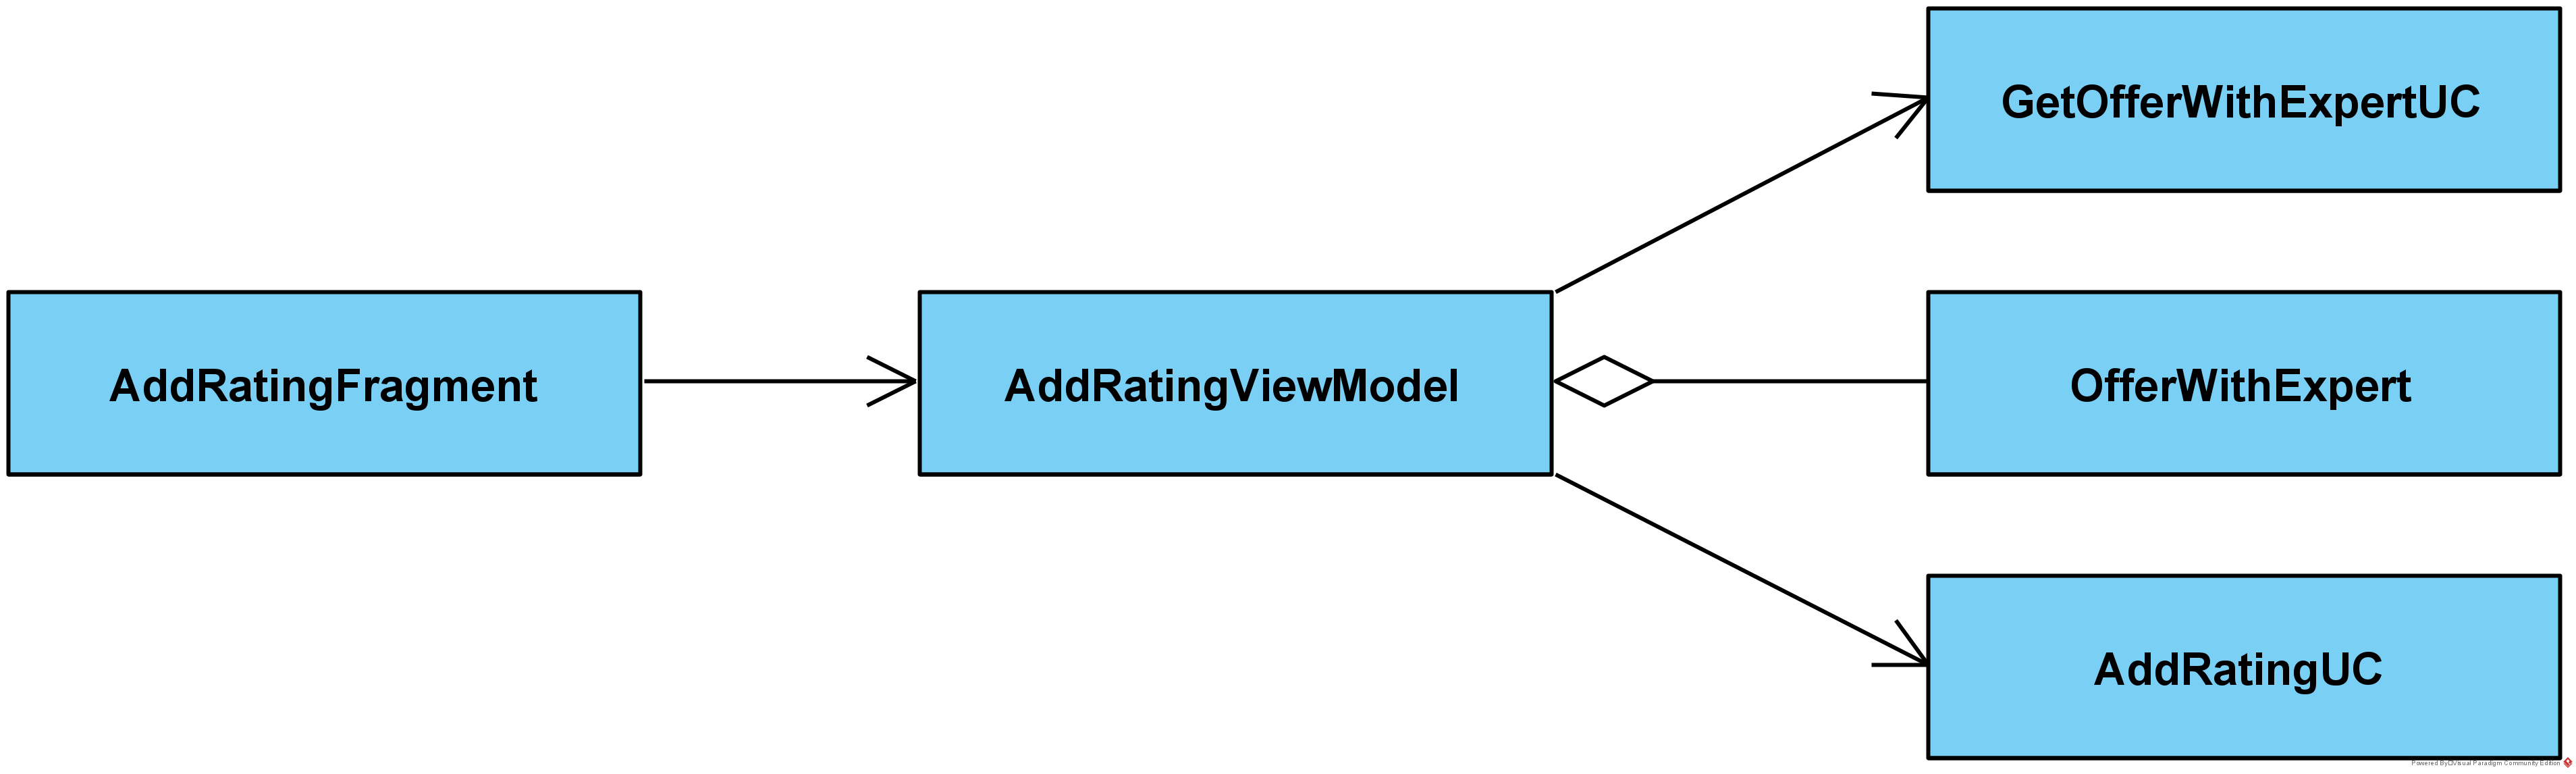
\includegraphics[width=\linewidth]{images/mvvm_example.png}
%   \caption{Wzorzec MVVM na przykładzie dodawania oceny}
%   \label{fig:mvvm-example}
% \end{figure}

% Na rysunku \ref{fig:mvvm-example} przedstawione zostało wykorzystanie wzorca MVVM na przykładzie dodawania oceny przez klienta. Klasa AddRatingViewModel stanowi ViewModel i zaczyna od wykonania przypadek użycia GetOfferWithExpertUC by dostać obiekt domenowy OfferWithExpert reprezentujący ofertę i wykonawcę, którego ma dotyczyć dodawana ocena. Zaktualizowanie tych wartości jest zauważane przez widok dzięki mechanizmowi subskrypcji i aktualizuje on natychmiastowo swoją zawartość. Gdy użytkownik uzupełni już ocenę i wciśnie przycisk potwierdzenia to widok poinformuje o tym ViewModel poprzez wywołanie jego odpowiedniej metody, który wykona przypadek użycia AddRatingUC i ocena zostanie dodana.

\section{Warstwa danych}
\label{wzorzec-repozytorium}

% Warstwa danych została zaimplementowana jako zbiór jedenastu repozytoriów. Stanowią one sposób na zapewnienie abstrakcji dostępu do danych i wszelkie operacje na danych mogą być wykonywane jedynie za ich pomocą. Zapewnia to spójność aplikacji i łatwość wprowadzania ewentualnych zmian w sposobie przechowywania informacji. Wszystkie repozytoria wraz z metodami, które posiadają, zostały przedstawione w postaci diagramu na rysunku \ref{fig:repos}.

Warstwa danych została zaimplementowana jako zbiór jedenastu repozytoriów, które stanowią sposób na zapewnienie abstrakcji dostępu do informacji. Umożliwia to dokonywanie zmian w sposobie przechowywania danych bez wpływu na logikę, która z nich korzysta.
Wszelkie operacje odczytu i modyfikacji wykonywane są jedynie za ich pomocą. Oznacza to, że pełnią rolę pojedynczego źródła prawdy (ang. Single Source of Truth). Zapewnia to spójność wyświetlanych przez aplikację informacji. Wszystkie repozytoria wraz z metodami, które posiadają, zostały przedstawione w postaci diagramu na rysunku \ref{fig:repos}.

\begin{figure}[ht!]
  \centering
  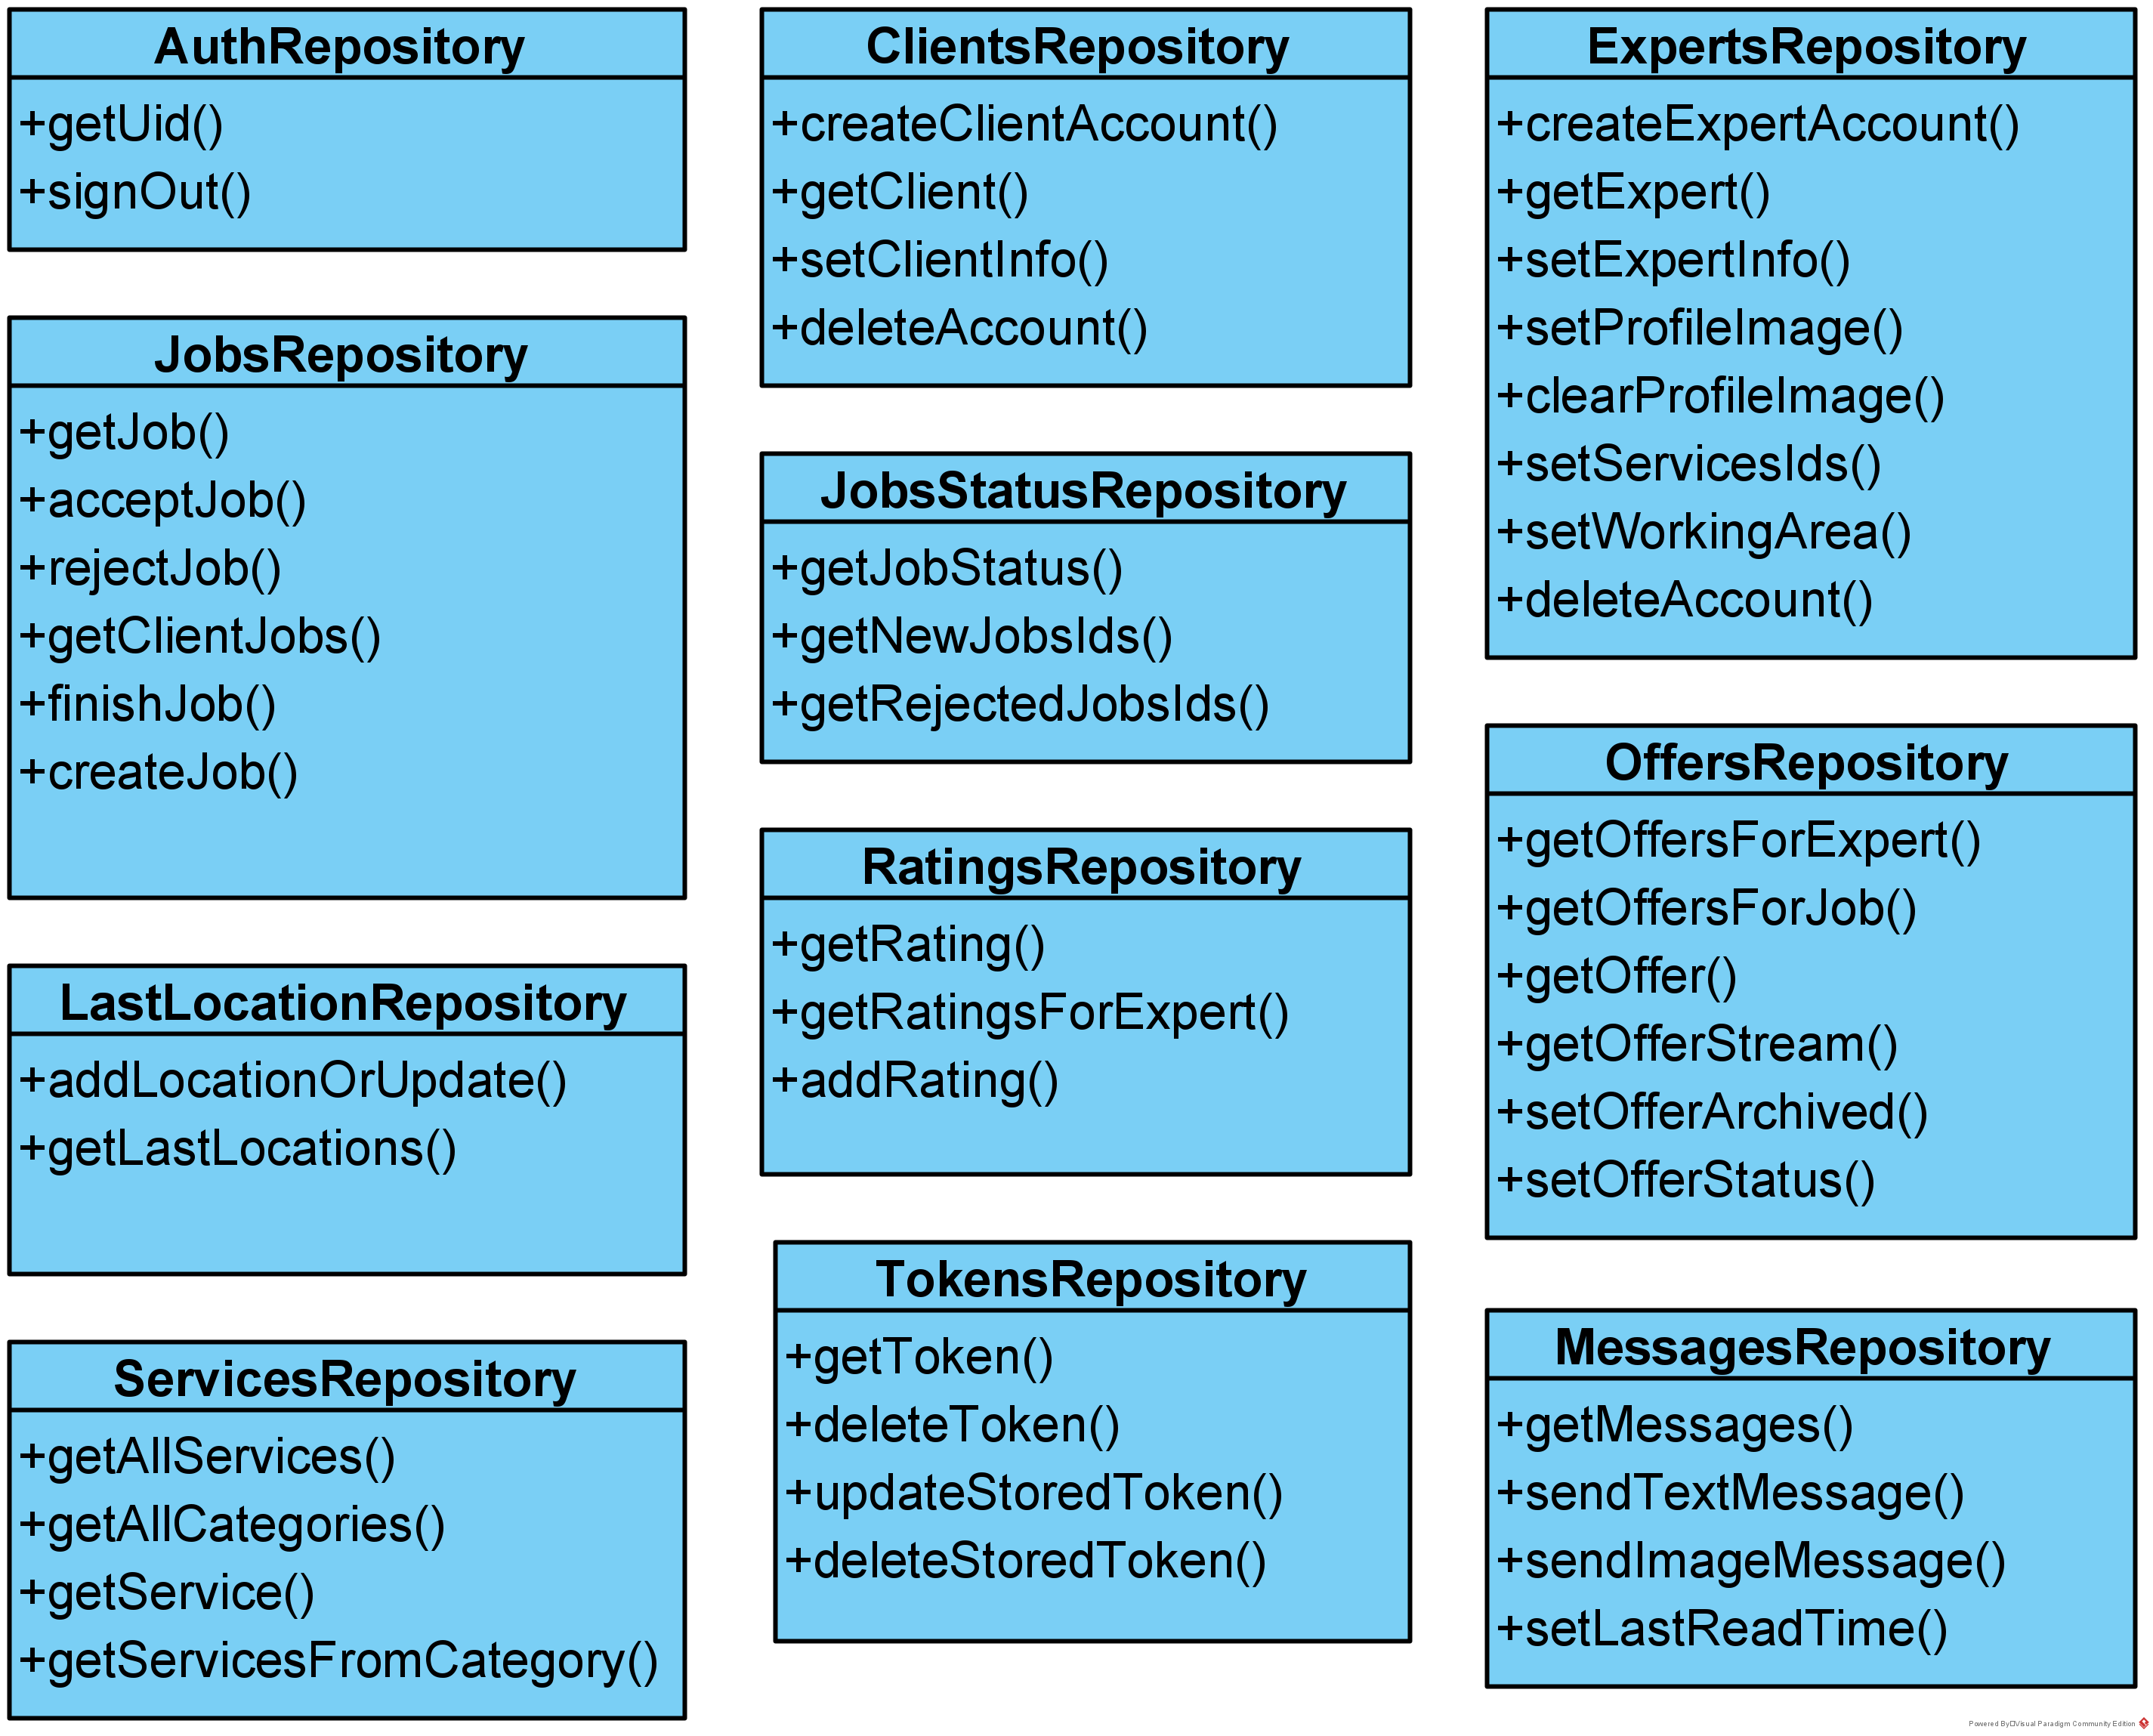
\includegraphics[width=\linewidth]{images/repositories.png}
  \caption{Diagram UML klas repozytoriów}
  \label{fig:repos}
\end{figure}

Każde repozytorium zostało stworzone z myślą o zarządzaniu konkretnym typem danych. Są one następujące:
\begin{itemize}
    \item \textbf{\code{AuthRepository}} - dane autoryzacji;
    \item \textbf{\code{ClientsRepository}} - klienci;
    \item \textbf{\code{ExpertsRepository}} - wykonawcy;
    \item \textbf{\code{JobsRepository}} - zlecenia;
    \item \textbf{\code{JobsStatusRepository}} - statusy zleceń, czyli informacje o ich dostępności z punktu widzenia konkretnych wykonawców;
    \item \textbf{\code{LastLocationsRepository}} - ostatnio użyte podczas dodawania zleceń lokalizacje;
    \item \textbf{\code{RatingsRepository}} - oceny wystawiane przez klientów;
    \item \textbf{\code{OffersRepository}} - oferty;
    \item \textbf{\code{ServicesRepository}} - usługi oraz kategorie usług;
    \item \textbf{\code{TokensRepository}} - tokeny FCM, wykorzystywane do notyfikacji push;
    \item \textbf{\code{MessagesRepository}} - wiadomości z chatu.
\end{itemize}

Wewnętrznie, aby wykonywać swoje zadania, repozytoria wykorzystują źródła danych. W aplikacji przewidziane zostały dwa źródła: lokalna baza danych ROOM oraz Firebase, przez który rozumiane są wszystkie dostępne w jego ramach usługi. Zostało to przedstawione na rysunku \ref{fig:data-sources}.

\begin{figure}[ht]
  \centering
  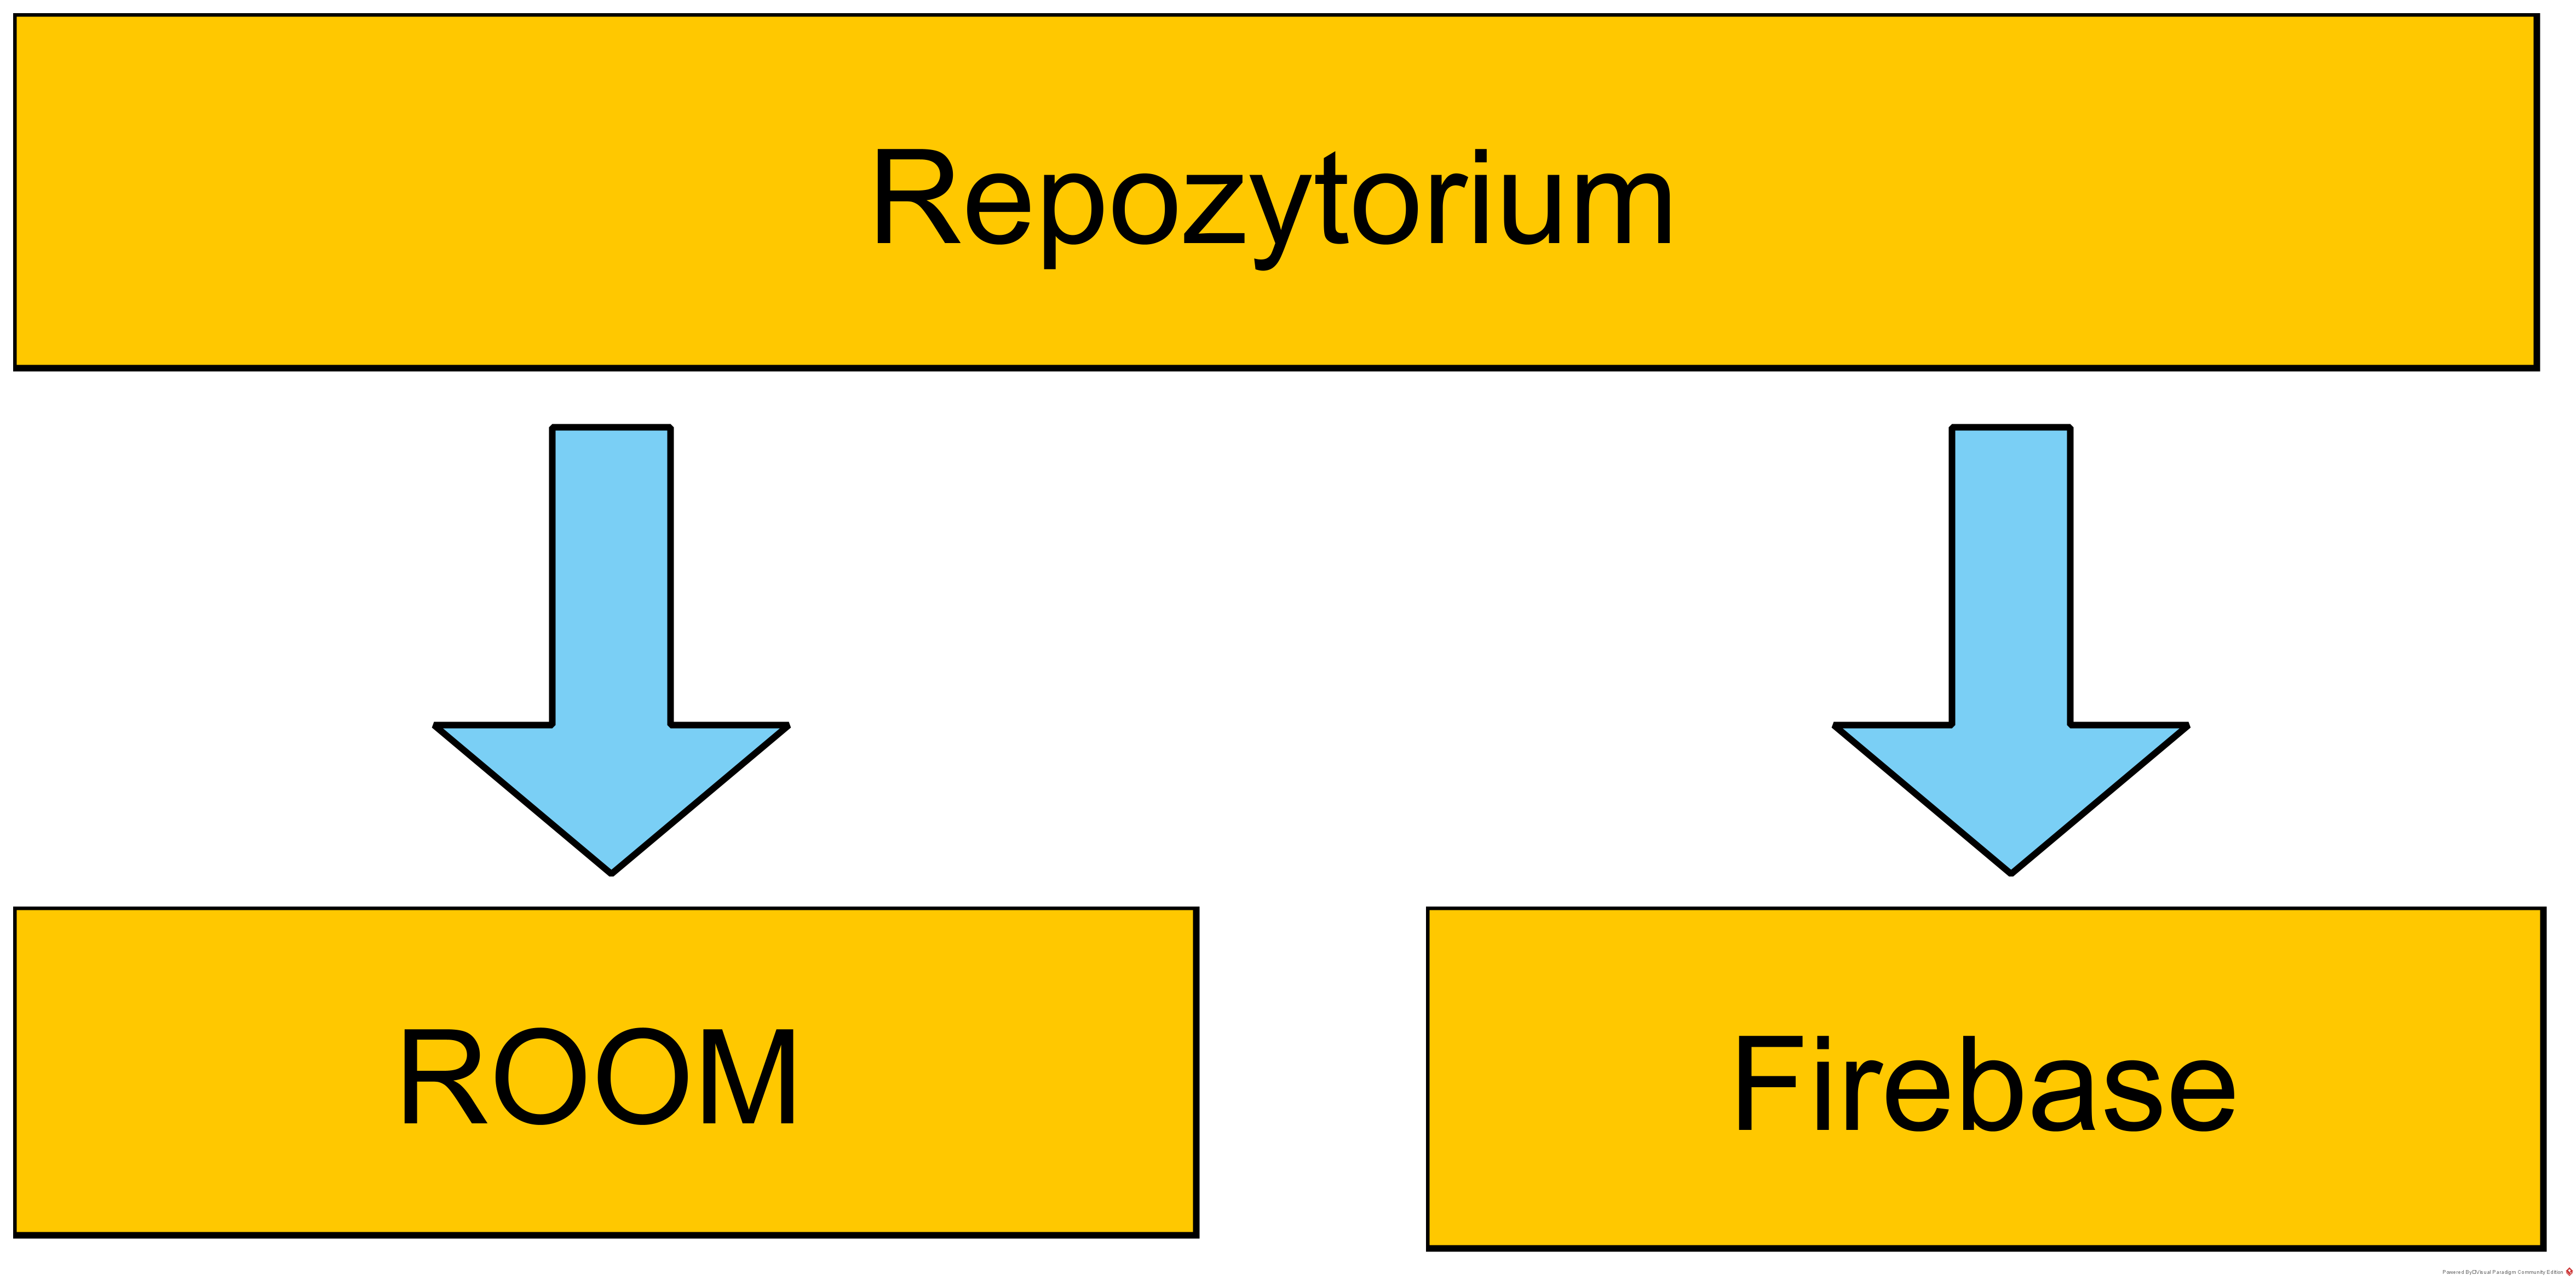
\includegraphics[width=0.7\linewidth]{images/data_sources.png}
  \caption{Schemat wykorzystania źródeł danych przez repozytoria}
  \label{fig:data-sources}
\end{figure}

W zależności od potrzeby repozytoria wykorzystują jedno lub oba źródła danych. Repozytorium \code{LastLocationsRepository}, zarządzające ostatnio wybieranymi lokalizacjami, wymaga jedynie lokalnej bazy ROOM, ponieważ są to informację, które mogą być zapisywane tylko lokalnie, a ich przechowywanie w zdalnej bazie danych jest zbędne. Repozytorium \code{MessagesRepository} wykorzystuje z kolei jedynie Firebase, ponieważ wiadomości z chatu muszą być dodawane i pobierane ze zdalnej bazy danych, by mogły być współdzielone pomiędzy użytkownikami. Korzystanie z bazy ROOM nie jest tutaj dodatkowo potrzebne, ponieważ używana baza Firebase Firestore posiada wbudowany mechanizm cachowania. Repozytorium \code{JobsStatusRepository} potrzebuje już jednak obu źródeł danych, ponieważ statusy zleceń są pobierane z Firebase przy pomocy funkcji Firebase Functions, które nie posiadają wbudowanego cachowania i pożądane jest wykorzystanie również lokalnej bazy danych ROOM, by je zapewnić.

\section{Współdzielenie kodu}
\label{code-sharing}

Na szczególną uwagę zasługują rozwiązania, które wykorzystano w celu minimalizacji duplikacji kodu pomiędzy aplikacjami dla klientów oraz wykonawców. Obie zawierają bowiem często podobne ekrany, które różnią się pewnymi zachowaniami, kolorami lub innymi nielicznymi elementami. 

O potrzebie unikania powtórzeń w kodzie mówi stosowana przez programistów reguła DRY (ang. Don't Repeat Yourself), która została sformułowana przez Andy'ego Hunta oraz Dave'a Thomasa w książce \enquote{Pragmatyczny programista} \cite{pragmatic-programmer}. Pomaga ona uniknąć błędów powstających podczas wielokrotnego wykonywania tej samej czynności oraz oszczędza czas.

Podstawowym działaniem jakie poczyniono w kierunku uniknięcia duplikacji kodu jest podział na trzy moduły, które zostały przedstawione na rysunku \ref{fig:moduły}. Moduły client oraz expert to moduły aplikacji. Są one zależne od moduł common, który jest modułem bibliotecznym, w którym zdecydowano się umieszczać współdzielony kod. 

\begin{figure}[ht!]
  \centering
  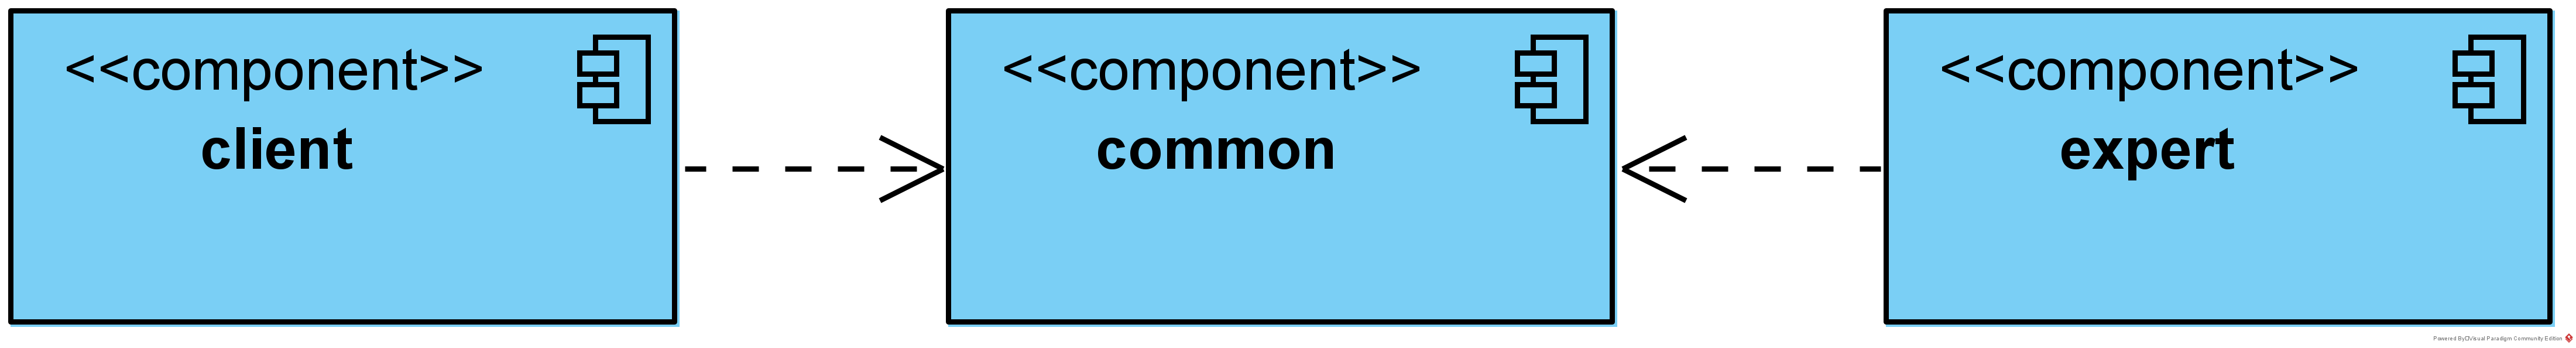
\includegraphics[width=\linewidth]{images/modules.png}
  \caption{Diagram UML przedstawiający stworzone moduły i ich relacje}
  \label{fig:moduły}
\end{figure}

W module common zostały umieszczone między innymi wszystkie repozytoria składające się na warstwę danych oraz wszystkie modele domenowe, ponieważ są to elementy, które w zdecydowanej większości są wykorzystywane w obu aplikacjach. Niektóre z nich są w rzeczywistości potrzebne tylko w jednej, lecz takich elementów jest na tyle mało, że zdecydowano się ich nie rozdzielać w celu utrzymania prostoty.

Na rysunku \ref{fig:dziedziczenie} przedstawiony został diagram UML przedstawiający sposób wykorzystania tych modułów na przykładzie ekranów usuwania konta klienta i wykonawcy. Ekrany te są do siebie wyraźnie podobne, różnią się jedynie kolorami, treścią wyświetlanych wiadomości oraz usuwaniem różnych obiektów.

\begin{figure}[ht!]
  \centering
  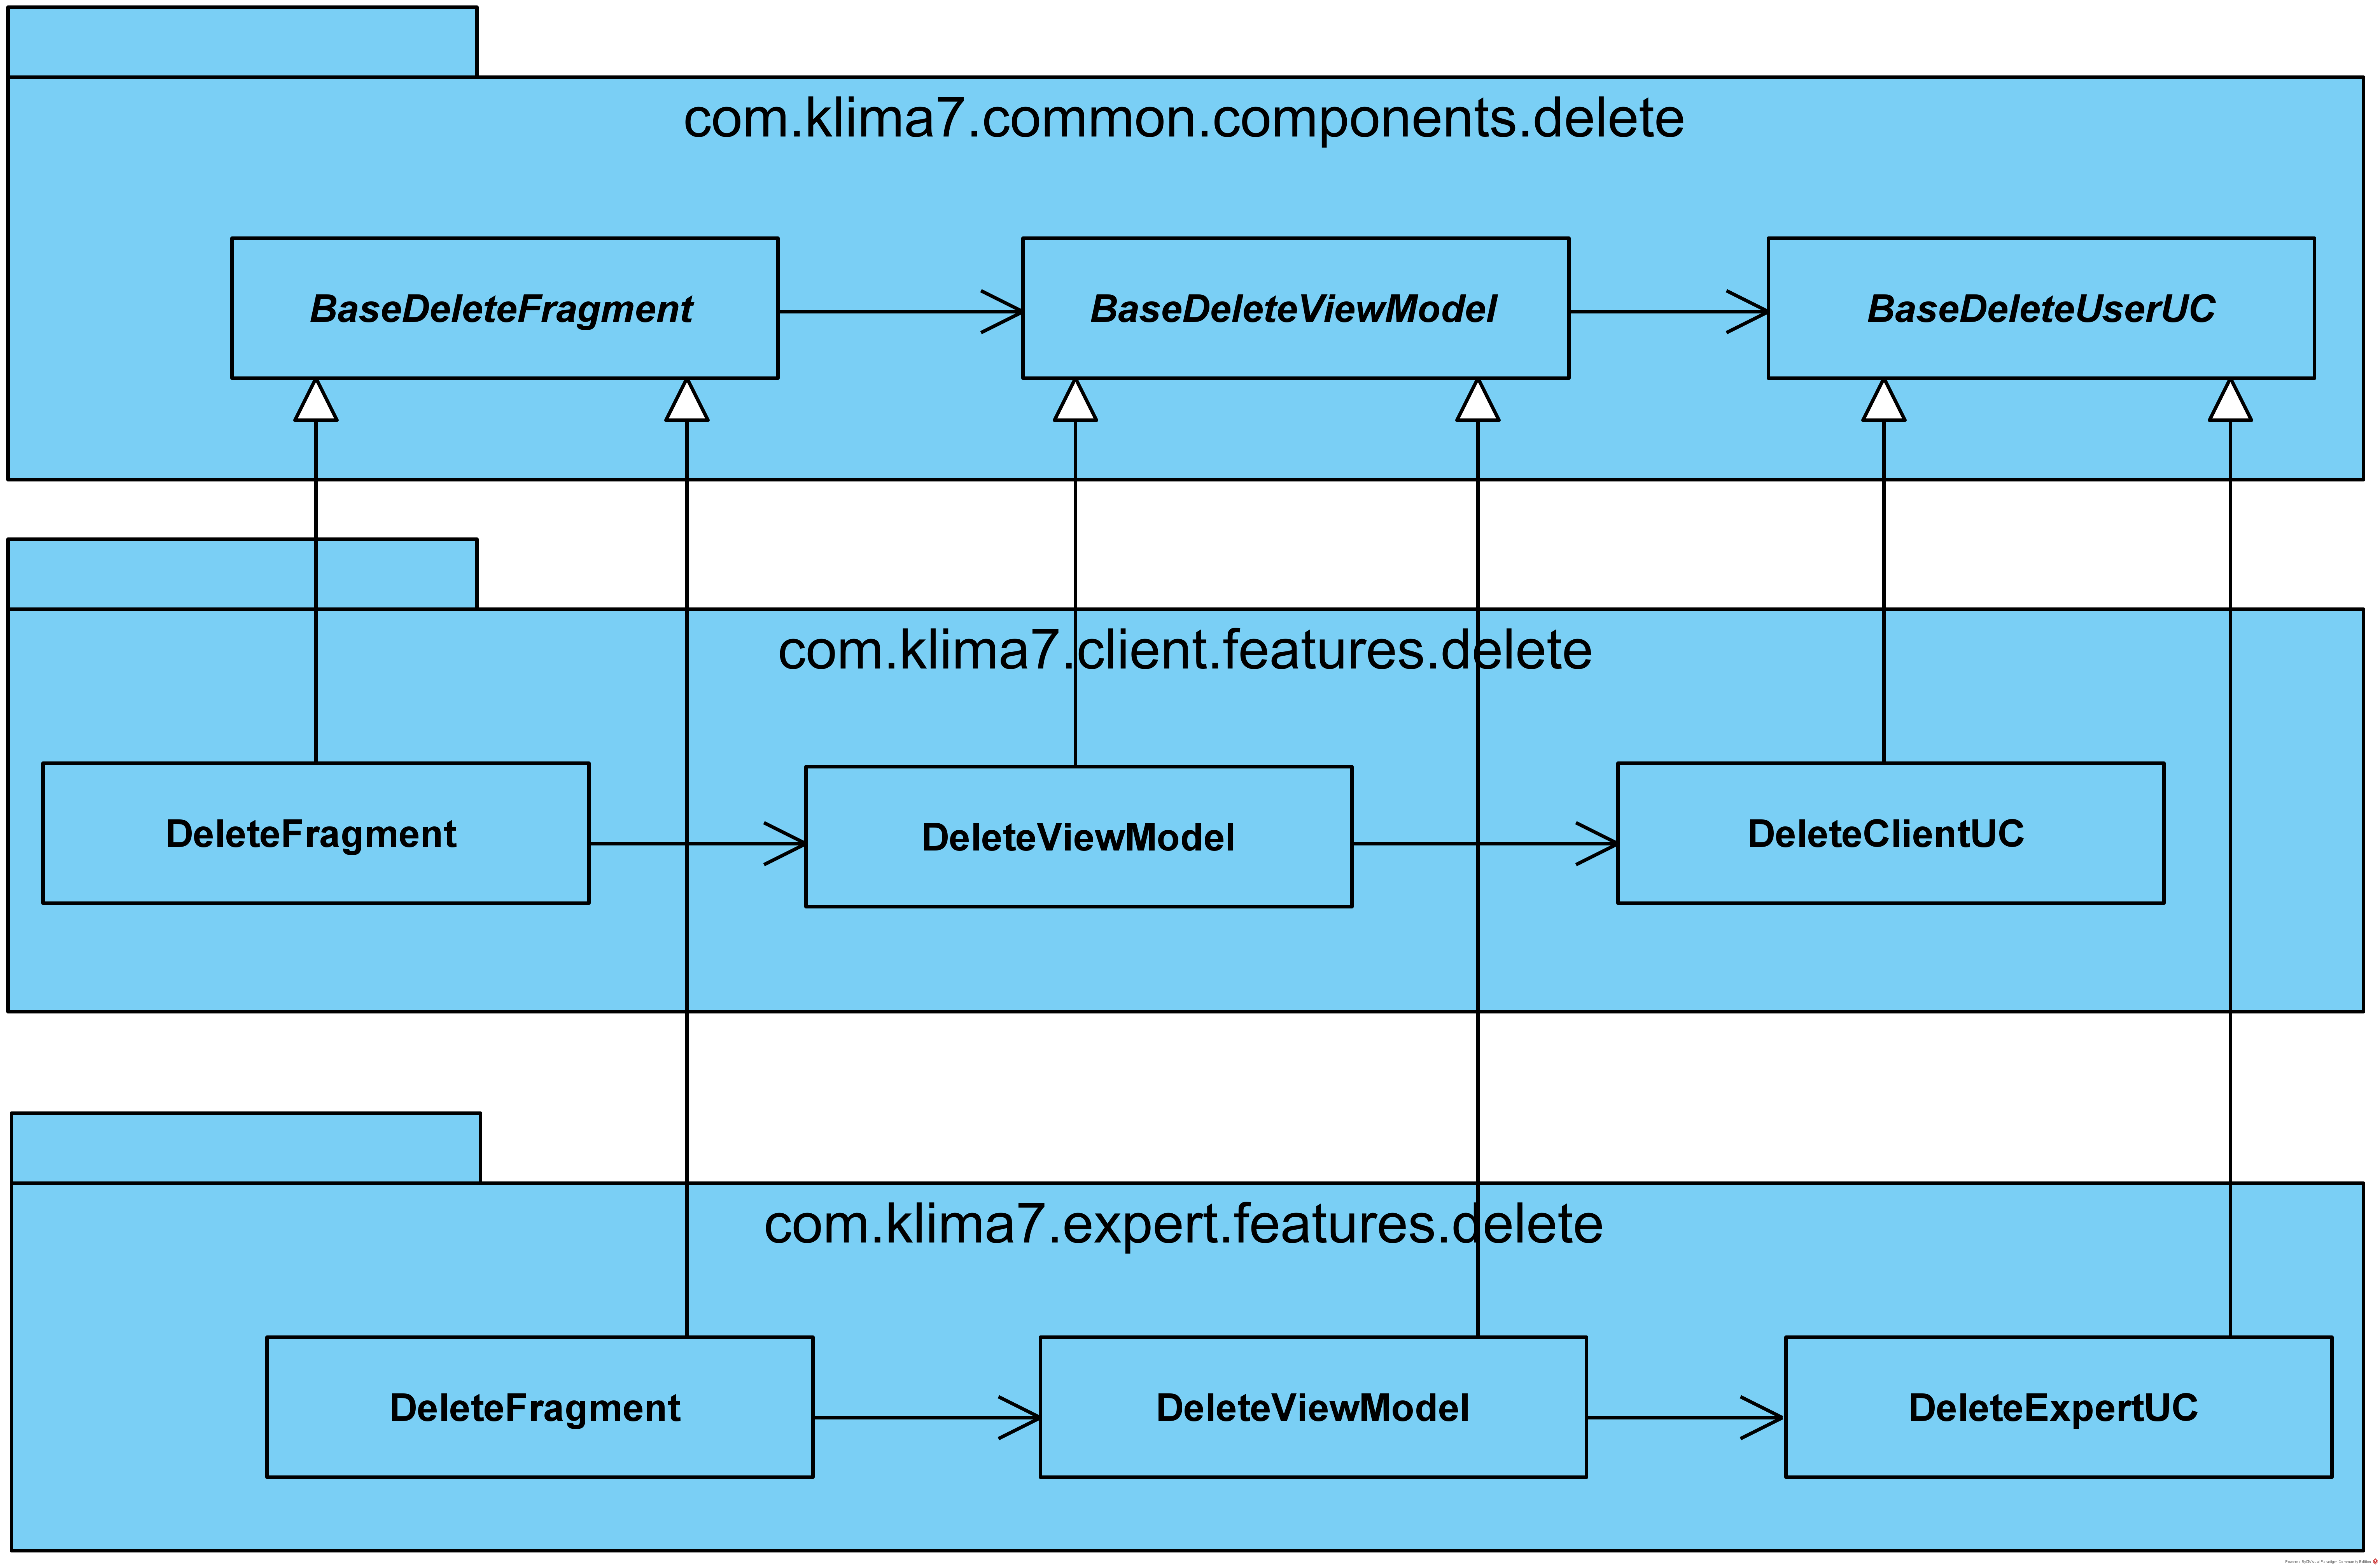
\includegraphics[width=\linewidth]{images/modules_example.png}
  \caption[Diagram UML prezentujący wykorzystanie modułów na przykładzie]{Diagram UML prezentujący wykorzystanie modułów dla współdzielenia kodu na przykładzie ekranów usuwania użytkowników}
  \label{fig:dziedziczenie}
\end{figure}

W celu zaimplementowania ekranów usuwania w module common zostały stworzone klasy bazowe. \code{BaseDeleteFragment} stanowi widok, \code{BaseDeleteViewModel} stanowi ViewModel, a \code{BaseDeleteUserUC} jest przypadkiem użycia usuwającym użytkownika. Są to jednak klasy abstrakcyjnie, co widać na diagramie UML po pochylonej czcionce. Oznacza to, że nie można ich bezpośrednio wykorzystać i konieczne jest ich rozszerzenie, co ma miejsce w modułach client oraz expert, gdzie podczas dziedziczenia dodawany jest do nich specyficzny dla danej aplikacji kod. W podobny sposób zostały zrealizowane również inne ekrany, które występują w dwóch alternatywnych wersjach.
% Backend
\chapter{Projekt Firebase}
\label{part:firebase}

Oprócz stworzenia samych aplikacji mobilnych realizacja tematu wymagała napisania kodu w ramach projektu Firebase, który odgrywa rolę backendu. Zaletą tego środowiska i tym co je odróżnia od aplikacji klienckich jest to, że jest ono w pełni kontrolowane. W związku z tym stanowi odpowiednie miejsce do wykonywania operacji, które wymagają szczególnego bezpieczeństwa czy spójności.

Podstawowa struktura projektu została wygenerowana automatycznie podczas procesu inicjalizacji, wspomaganego przeznaczonym do tego celu narzędziem. Jest ona dość prosta i została przedstawiona na rysunku \ref{fig:firebase-struktura}.

\begin{figure}[ht!]
  \centering
  \fbox{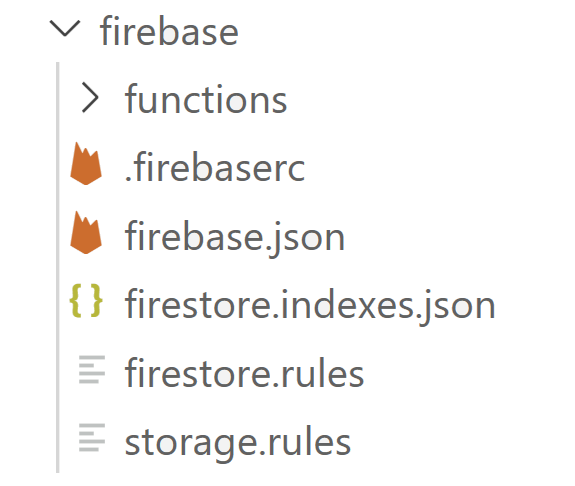
\includegraphics[width=0.6\linewidth]{images/firebase_structure.png}}
  \caption{Schemat struktury projektu Firebase}
  \label{fig:firebase-struktura}
\end{figure}

Pliki \filename{.firebaserc} oraz \filename{firebase.json} są plikami konfiguracyjnymi w formacie JSON. Pierwszy zawiera identyfikator projektu, a drugi konfigurację poszczególnych usług. Ich zawartość po poprawnej inicjalizacji wymagała jedynie delikatnych poprawek.

Katalog \filename{functions} przechowuje kod funkcji Firebase Functions. Jest to zdecydowanie najbardziej obszerna część projektu Firebase i jego zawartość zostanie opisana dokładnie w sekcji \ref{projekt-funkcje}.

Plik \filename{firestore.indexes.json} zawiera indeksy bazy danych Firestore, przechowywane w formacie JSON. Plik ten nie był edytowany manualnie, ze względu na swoją dość skomplikowaną strukturę. Zamiast tego indeksy były tworzone za pomocą wygodnego interfejsu dostępnego przy pomocy przeglądarki internetowej, a następnie wprowadzane do wspomnianego pliku odpowiednią komendą wiersza poleceń. Posiadanie ich bowiem w pliku \filename{firestore.indexes.json} umożliwia stworzenie wszystkich na raz, zamiast mozolnego dodawania przy pomocy przeglądarki. Okaże się to bardzo przydatne w przypadku potrzeby ponownego wdrożenia projektu.

Ostatnie dwa pliki, czyli \filename{firestore.rules} oraz \filename{storage.rules} zawierają reguły bezpieczeństwa Firebase Security Rules, odpowiednio dla bazy Firestore i magazynu plików Cloud Storage. Zostaną one przedyskutowane w sekcji \ref{projekt-reguły}.

\section{Firebase Functions}
\label{projekt-funkcje}

Funkcje są fragmentami kodu, które mogą być wykonywane w odpowiedzi na różne zdarzenia i wywoływać inne usługi. Wykorzystują środowisko Node.js i język TypeScript, a związany z nimi kod, znajdujący się w katalogu \filename{functions} projektu, tworzy typową dla tego środowiska strukturę. To co najważniejsze, czyli kod samych funkcji, umieszczony jest w podkatalogu \filename{src}.

Podczas pisania kodu wykorzystano narzędzie ESlint, które zapewnia jego statyczną analizę w celu wczesnego sygnalizowania błędów. Ponadto ułatwia utrzymanie spójności stosowanych konwencji, takich jak poprzedzanie nieużywanych parametrów znakiem podkreślenia, czy konsekwentne używanie wcięć.

W rozważanym projekcie wykorzystanych zostało 37 funkcji, które można podzielić na cztery kategorie: funkcje wywoływane bezpośrednio, wywoływane okresowo, poprzez modyfikację danych oraz poprzez modyfikację plików. 

\subsection{Funkcje wywoływane bezpośrednio}

Największą część funkcji stanowią te, które są wywoływane bezpośrednio przez aplikacje klienckie. Mogą wówczas zostać przekazane ewentualne argumenty, a w wyniku ich wykonania może zostać zwrócona wartość.

Alternatywę dla tego typu delegowania zadań do funkcji przez aplikacje mobilne stanowi bezpośrednie ich wykonanie po stronie klienckiej. Nie zawsze można jednak na to pozwolić, ponieważ przerwanie niektórych zadań może zostawić system w stanie niespójnym. Środowisko funkcji jest znacznie bezpieczniejsze i stanowi dobre miejsce na wykonywanie takich operacji. 

Ten rodzaj funkcji musiał również zostać wykorzystany do ustawiania przez aplikacje klienckie danych, z których walidacją nie były w stanie poradzić sobie reguły bezpieczeństwa Firebase Security Rules. W celu weryfikacji niektórych informacji konieczne było bowiem wykonanie żądania do API map, co dla reguł nie jest możliwe, a dla funkcji już tak. 

Ostatecznie, aby zachować spójność i nie wykonywać części operacji modyfikacji bezpośrednio w bazie, a części za pośrednictwem funkcji, postanowiono dla wszystkich preferować drugą możliwość. Bezpośrednich modyfikacji dokonywano natomiast jedynie wtedy, gdy było to naprawdę uzasadnione.

Na listingu \ref{lst:function-onCall} została przedstawiona przykładowa, bezpośrednio wywoływana funkcja, która służy do ustawiania obszaru świadczenia usług przez wykonawcę. Wymaga ona podania identyfikatora lokalizacji oraz długości promienia w kilometrach jako argumentów. Zostało to ukryte na listingu w celu jego uproszczenia, lecz korzysta ona z Google Geocoding API, aby sprawdzić poprawność identyfikatora i pobrać nazwę miejsca, a następnie dokonuje aktualizacji odpowiednich wartości w bazie danych.

\begin{minipage}{\linewidth}
\lstinputlisting[
caption=Funkcja wywoływana bezpośrednio, label={lst:function-onCall}
]{listings/function_invoked.ts}
\end{minipage}

Tego typu funkcje posiadają dwa parametry. Pierwszym są dane, które zostały przekazane podczas ich wywołania, a drugi zawiera dodatkowe informacje, z których najczęściej wykorzystywanym jest identyfikator wywołującego ją użytkownika.

W przypadku jawnie wywoływanych funkcji ważna jest walidacja danych, które zostały do nich przekazane. Należało każdorazowo sprawdzić, czy posiadają one odpowiednie typy oraz czy przyjmują odpowiednie wartości. W tym celu została wykorzystana biblioteka Joi, która znacznie ułatwia to zadanie poprzez możliwość definiowania schematów, na podstawie których poprawność parametrów mogła być łatwo oceniana.

Przykładowy schemat przedstawiony na listingu \ref{lst:function-invoke-schema} określa, że przekazane dane muszą zawierać dwie wymagane wartości: \code{placeId} oraz \code{radius}. Pierwsza musi być łańcuchem tekstowym o długości od 1 do 100 znaków, a druga liczbą całkowitą z zakresu pomiędzy 0 oraz \verb|MAX_AREA_RADIUS|. Ograniczenia te zostały wyrażone w czytelny oraz zwarty sposób, w przeciwieństwie do długich, powtarzalnych instrukcji warunkowych, które byłyby konieczne bez biblioteki Joi.

\begin{minipage}{\linewidth}
\lstinputlisting[
caption=Przykładowy schemat biblioteki Joi,
label={lst:function-invoke-schema}
]{listings/function_invoked_schema.ts}
\end{minipage}

\subsection{Funkcje wywoływane okresowo}

Funkcje wywoływane okresowo to takie, których wykonanie odbywa się periodycznie, o ustalonym czasie. Nie mogą być już wywoływane przez aplikacje klienckie, a dzieje się to samoistnie. Wykorzystano ich niewiele, lecz pełnią ważne role.

\begin{minipage}{\linewidth}
\lstinputlisting[
caption=Funkcja wywoływana okresowo,
label={lst:function-scheduled}
]{listings/function_scheduled.ts}
\end{minipage}

Na listingu \ref{lst:function-scheduled} została przedstawiona przykładowa funkcja wywoływana okresowo, która jest odpowiedzialna za zamykanie zleceń, których czas ważności minął. Jest on wyrażany z dokładnością co do dnia, więc wykonywanie jej raz na dobę o północy jest wystarczające. Czas ten jest zapisany w postaci wyrażenia \verb|0 0 * * *|, które wykorzystuje składnię crontab. Zostało ono wyjaśnione na rysunku \ref{fig:crontab}. Składnia ta nie zawsze jest czytelna, lecz daje duże możliwości. Dla każdej funkcji, oprócz wyrażonego w ten sposób czasu, ustalana jest również strefa czasowa na polską. Jest to konieczne, ponieważ domyślną jest strefa czasowa Los Angeles, co powoduje niechciane przesunięcie w czasie wykonywania.

\begin{figure}[ht!]
  \centering
  
\includegraphics[width=\linewidth]{images/crontab.png}
  \caption{Schemat wyjaśniający wykorzystane wyrażenie crontab}
  \label{fig:crontab}
\end{figure}

\subsection{Funkcje wywoływane modyfikacją danych}

Funkcje wywoływane modyfikacją danych są uruchamiane automatycznie w odpowiedzi na wykonanie określonej operacji w określonej części bazy Firebase Firestore. Mogą być uruchamianie po dodaniu dokumentu, jego usunięciu lub aktualizacji. Nasłuchiwanie tych operacji może być prowadzone dla konkretnych dokumentów lub całych kolekcji.

Głównym zastosowaniem omawianego rodzaju funkcji okazało się utrzymywanie spójności w bazie danych. Pomiędzy znajdującymi się w niej dokumentami istnieją bowiem pewne zależności, które należy egzekwować. Przykładem ich wykorzystania w tym kontekście jest aktualizacja średniej oceny wykonawcy po wykryciu dodania nowej, aktualizująca ostatnio wysłanej wiadomości po nadaniu kolejnej, czy usuwanie komentarzy wykonawcy po wykryciu jego usunięcia.

Poza utrzymywaniem spójności funkcje wywoływane modyfikacją danych okazały się również przydatne do wysyłania powiadomień do użytkowników. Przykładem tego jest nasłuchiwanie utworzenia nowego dokumentu w kolekcji wiadomości, by wysłać komunikat o nowej, nieodczytanej wiadomości do odpowiedniego użytkownika, gdy to nastąpi.

% Brak przecinka przed zamiast
Na listingu \ref{lst:function-firestore} przedstawiona została przykładowa funkcja, której zadanie polega na aktualizacji ostatnio wysłanej wiadomości, gdy zostanie dodana nowa. W tym celu nasłuchuje dodawania dokumentów, których lokalizacja pokrywa się z podaną ścieżką. Zawiera ona w dwóch miejscach nazwy w nawiasach klamrowych, zamiast identyfikatorów dokumentów. Oznaczają one, że dany jej fragment może zostać dopasowany do dowolnego dokumentu. Pierwszy argument z którym wywoływana jest funkcja stanowi zawartość nowo stworzonego dokumentu, a drugi zawiera między innymi identyfikator użytkownika dokonującego modyfikacji oraz fragmenty ścieżki, które zostały dopasowane do wspomnianych wcześniej nazw w nawiasach klamrowych. Dzięki tym argumentom wewnątrz ciała funkcji możliwa jest odpowiednia aktualizacja ostatniej wiadomości.

\begin{minipage}{\linewidth}
\lstinputlisting[
caption=Funkcja wywoływana modyfikacją danych,
label={lst:function-firestore}
]{listings/function_firestore.ts}
\end{minipage}

\subsection{Funkcje wywoływane modyfikacją plików}

Istotny rodzaj wykorzystywanych funkcji stanowią te, które są wywoływane modyfikacją plików przechowywanych w usłudze Firebase Storage. Przede wszystkim możliwe jest wykonywanie ich w odpowiedzi na dodawanie oraz usuwanie plików. Dostępne są również inne zdarzenia, które je uruchamiają, lecz nie zostały użyte.

Rozważane funkcje są wykorzystywane do synchronizacji pomiędzy usługą Firebase Cloud Storage, przechowującą pliki, a bazą danych. Można to rozważyć na przykładzie zdjęć profilowych. Gdy wykonawca ustawia swoje zdjęcie, to jest ono wysyłane przez aplikację kliencką bezpośrednio do Cloud Storage. W tej chwili dodawanie pliku wywołuje wykonanie funkcji, która aktualizuje w bazie danych informacje dotyczące zdjęcia profilowego, czyli jego adres URL oraz datę zmiany. Podobnie, gdy wykonawca usuwa zdjęcie, to aplikacja kliencka usuwa je bezpośrednio z usługi magazynu plików. Jest to następnie wykrywane przez funkcję, która odpowiednio aktualizuję dane wewnątrz Firestore.

Na listingu \ref{lst:function-storage} została przedstawiona funkcja, która aktualizuje bazę danych po usunięciu zdjęcia profilowego. Jest ona w rzeczywistości wykonywana po usunięciu każdego pliku i nie ma możliwości zawężenia nasłuchiwanego przez nią obszaru jedynie do katalogu zdjęć profilowych. Parametr z którym jest wywoływana umożliwia jednak uzyskanie ścieżki do pliku, który spowodował jej wykonanie i na tej podstawie można stwierdzić, czy rzeczywiście jest to zdjęcie profilowe.

\begin{minipage}{\linewidth}
\lstinputlisting[
caption=Funkcja wywoływana modyfikacją plików,
label={lst:function-storage}
]{listings/function_storage.ts}
\end{minipage}

Wewnątrz funkcji wywoływanych modyfikacją plików nie jest możliwe uzyskanie identyfikatora użytkownika, który dokonał zmiany. Fakt ten okazał się dla autora dość zaskakujący, ponieważ wydaje się to być jedną z podstawowych informacji, a funkcje wywoływane modyfikacją bazy Firestore z jakichś powodów już ją udostępniają, co wydaje się niekonsekwentne. Obejściem tego problemu okazało się stworzenie katalogów o nazwach odpowiadających identyfikatorom użytkowników, a następnie ograniczenie im dostępu za pomocą Firebase Security Rules jedynie do swoich folderów. Dzięki temu analizując ścieżkę zmodyfikowanego pliku można było uzyskać informację o użytkowniku, który tego dokonał.

\section{Firebase Security Rules}
\label{projekt-reguły}

Firebase Security Rules to reguły, które pozwalają na ograniczenie aplikacjom klienckim dostępu do danych przechowywanych przez Firebase. Usługami dla których określono reguły są Firestore oraz Cloud Storage. Było to konieczne, aby zapewnić bezpieczeństwo dla bazy danych oraz magazynu plików.

Pozornie określanie reguł bezpieczeństwa może wydawać się niepotrzebne, ponieważ już sama logika aplikacji klienckich została zaprojektowana w taki sposób, aby uniemożliwić niechciane scenariusze. Nie jest to jednak wystarczające, ponieważ należy mieć na uwadze możliwość ingerencji w aplikacje niepożądanych osób lub zdobycia przez nie w inny sposób dostępu, w celu uzyskania pewnych korzyści, kradzieży danych czy spowodowania awarii aplikacji. Poza tym zawsze istnieje możliwość popełnienia błędów w logice aplikacji przez programistę, a kolejna warstwa zabezpieczeń, w postaci Firebase Security Rules, pozwala zablokować te operacje, które nie powinny mieć miejsca.

Stworzone reguły mają zastosowanie jedynie do aplikacji klienckich. W żaden sposób nie wpływają one na operacje, które mogą być wykonywane w ramach Firebase Functions. Dzieje się tak, ponieważ środowisko, w którym funkcje są wykonywane, jest uważane za środowisko w pełni kontrolowane, a więc bezpieczne.  

\subsection{Reguły dla Firebase Firestore}

Reguły bezpieczeństwa dla Firestore działają na poziomie dokumentów i umożliwiają określenie osobnych uprawnień dla operacji odczytu oraz zapisu. Jeżeli potrzebny jest większy poziom szczegółowości uprawnień to zapis może zostać rozbity na uprawnienia do tworzenia, aktualizacji oraz usuwania. Najważniejsze wprowadzone reguły są następujące:

\begin{itemize}
    \item Dla kolekcji zawierających usługi oraz kategorie usług uniemożliwiono zapis, ponieważ zawierają wartości, których zmian nie przewidziano.
    \item Dla kolekcji matchings, która stanowi jedynie szczegół implementacyjny, zarówno zapis, jak i odczyt został zablokowany.
    \item Na odczyt wiadomości zezwolono jedynie użytkownikowi będącemu jego nadawcą lub odbiorcą.
    \item Na odczyt oferty zezwolono jedynie wykonawcy, który ją złożył oraz klientowi, któremu została złożona.
\end{itemize}

% TODO: Można wspomnieć o braku możliwości stworzenia ograniczenia na joby

Ograniczeniem, które okazało się problemem, jest to, że można uniemożliwić odczyt jedynie dla całych dokumentów, a nie można tego zrobić na poziomie poszczególnych ich pól. W związku z tym nie udało się zablokować odczytu tych, które stanowią jedynie szczegóły implementacyjne. Przykładem takich pól są dwa znajdujące się w dokumentach wykonawców, przechowujące sumę oraz liczbę ocen. Są wykorzystywane jedynie w celu wyliczenia średniej oceny i nie są używane przez aplikacje klienckie, a pomimo tego będą one miały do nich dostęp.

Rozwiązaniem problemu pól będących szczegółami implementacyjnymi mogłoby być przeniesienie ich do osobnych dokumentów oraz kolekcji, dla których dostęp mógłby zostać już ograniczony. Takie podejście rozwiązałoby go, lecz wiązałoby się z powstaniem dużej liczby dodatkowych kolekcji, zwiększających stopień komplikacji projektu. Biorąc pod uwagę, że rozważane pola nie przechowują żadnych krytycznych danych i ich udostępnienie nie powinno stanowić zagrożenia bezpieczeństwa ani prywatności, zdecydowano się to zaakceptować.

\subsection{Reguły dla Firebase Cloud Storage}

Reguły wykorzystywane przez Firebase Cloud Storage działają na poziomie plików i umożliwiają określanie osobnych zasad dla ich odczytu i zapisu. Gdy nie jest to wystarczające, to zapis można doprecyzować przy pomocy reguł tworzenia, aktualizacji i usuwania.

Przez usługę przechowywane są jedynie dwa typy danych: zdjęcia profilowe oraz obrazy wysyłane przez chat. Z tego powodu liczba reguł wymagana przez nią okazała się znacznie mniejsza niż w przypadku Firestore. 

Stworzone reguły ograniczają możliwość dodawania plików jedynie do przeznaczonych dla tego celu katalogów. Określają, że w przypadku zdjęć profilowych możliwe są wszystkie operacje zapisu, ponieważ wykonawcy mogą dodawać, aktualizować oraz usuwać swoje zdjęcia. Dodatkowo wymagają, aby nazwy plików przesyłanych do katalogu zdjęć profilowych stanowiły identyfikatory użytkowników połączone z rozszerzeniem png. Jeżeli któreś z wymagań nie będzie spełnione, to operacja zostanie odrzucona.
W przypadku zdjęć wysyłanych przez chat, poza koniecznością umieszczenia ich w odpowiednim katalogu, wymagane jest posiadanie przez nie rozszerzenia png. Ponadto możliwe operacje są ograniczone jedynie do tworzenia nowego pliku, ponieważ nie przewidziano możliwości aktualizowania, ani usuwania już wysłanego przez chat zdjęcia

\chapter{Funkcjonalności}

W niniejszym rozdziale przedstawione zostaną wszystkie zaimplementowane funkcjonalności jedna po drugiej. Zamieszczono je w takiej kolejności, aby ułatwić ich zrozumienie, poprzez uwzględnienie istniejących pomiędzy nimi zależności. Zostaną wsparte odpowiednimi zrzutami ekranów z aplikacji, które je prezentują. Część funkcjonalności ma zastosowanie tylko do jednej z aplikacji, a część do obu, co zostanie wyraźnie podkreślone.

\section{Motywy kolorystyczne}

W celu odróżnienia od siebie obu aplikacji postanowiono zastosować dla nich różne motywy kolorystyczne. Mają one wpływ na wszystkie ekrany, które można zobaczyć w dalszej części rozdziału, jak i na ikony, które przedstawiono na rysunku \ref{fig:icons}.

\begin{figure}[ht!]
  \centering
  \fbox{
\includegraphics[width=0.6\linewidth]{images/icons.png}}
  \caption{Ikony stworzonych aplikacji}
  \label{fig:icons}
\end{figure}

Motywy są stałe i nie można ich zmieniać, lecz poprzez to ułatwiają pracę użytkownikom, którzy posiadają zainstalowane obie aplikacje. Gdyby nie one, to ze względu na wiele podobieństw użytkownicy mogliby zostać zdezorientowani i mylić aplikacje w której aktualnie się znajdują.

Wybór koloru zielonego oraz niebieskiego jako motywów odpowiednio aplikacji dla klientów oraz wykonawców nie stanowi przypadku. Zgodnie z artykułem napisanym przez Hermana Cerato \cite{colors-meaning} każdy kolor ma inne znaczenie i zastosowanie. Skupia się on w szczególności na znaczeniu kolorów w domenie biznesowej. Według przytoczonego dokumentu kolor zielony jest kojarzony z harmonią, ma silny emocjonalny związek z poczuciem bezpieczeństwa i stabilności. Kolor niebieski za to najsilniej ze wszystkich jest wiązany z zaufaniem i niezawodnością. Wymienione pozytywne skojarzenia czynią wybrane barwy odpowiednimi do zastosowania w tworzonych aplikacjach.
\section{Podstawowe ekrany}

W pierwszej kolejności opisane zostaną trzy podstawowe ekrany, które są obecne w obu aplikacjach. Są to ekrany powitalne, ustawień oraz podziękowań. Ich wygląd w aplikacji dla wykonawców został przedstawiony na rysunku \ref{fig:basic-expert}.

% \begin{figure}[ht]
%   \captionsetup[subfigure]{justification=centering}
%   \centering
%   \begin{subfigure}{0.32\textwidth}
%     \centering
%     \fbox{
\includegraphics[width=0.97\linewidth]{screens/splash_client.png}}
%     \caption{Ekran powitalny}
%   \end{subfigure}
%   \begin{subfigure}{0.32\textwidth}
%     \centering
%     \fbox{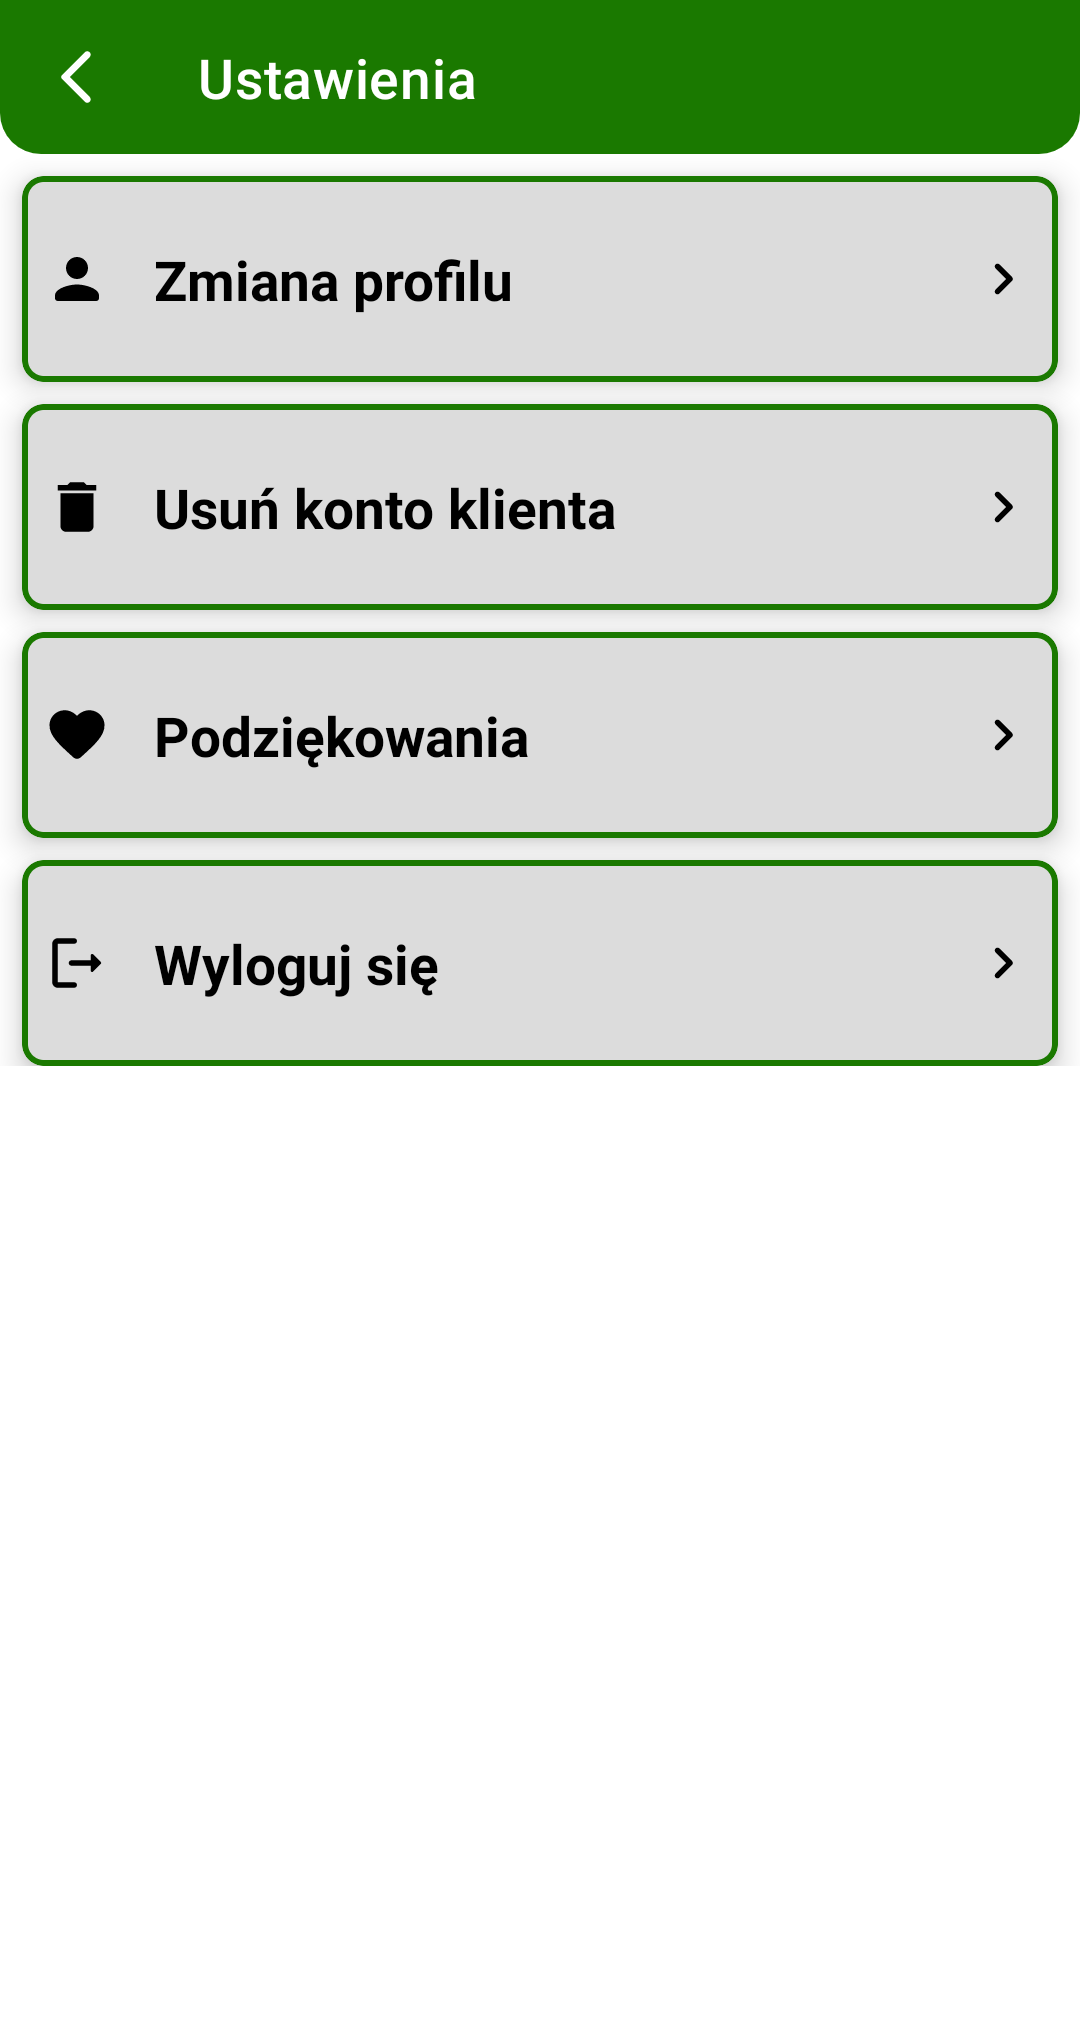
\includegraphics[width=0.97\linewidth]{screens/settings_client.png}}
%     \caption{Ekran ustawień}
%   \end{subfigure}
%   \begin{subfigure}{0.32\textwidth}
%     \centering
%     \fbox{
\includegraphics[width=0.97\linewidth]{screens/credits_client.png}}
%     \caption{Ekran podziękowań}
%   \end{subfigure}
%   \caption{Podstawowe ekrany aplikacji dla klientów}
%   \label{fig:basic-client}
% \end{figure}

\begin{figure}[ht]
  \captionsetup[subfigure]{justification=centering}
  \centering
  \begin{subfigure}{0.32\textwidth}
    \centering
    \fbox{
\includegraphics[width=0.97\linewidth]{screens/splash_expert.png}}
    \caption{Ekran powitalny}
  \end{subfigure}
  \begin{subfigure}{0.32\textwidth}
    \centering
    \fbox{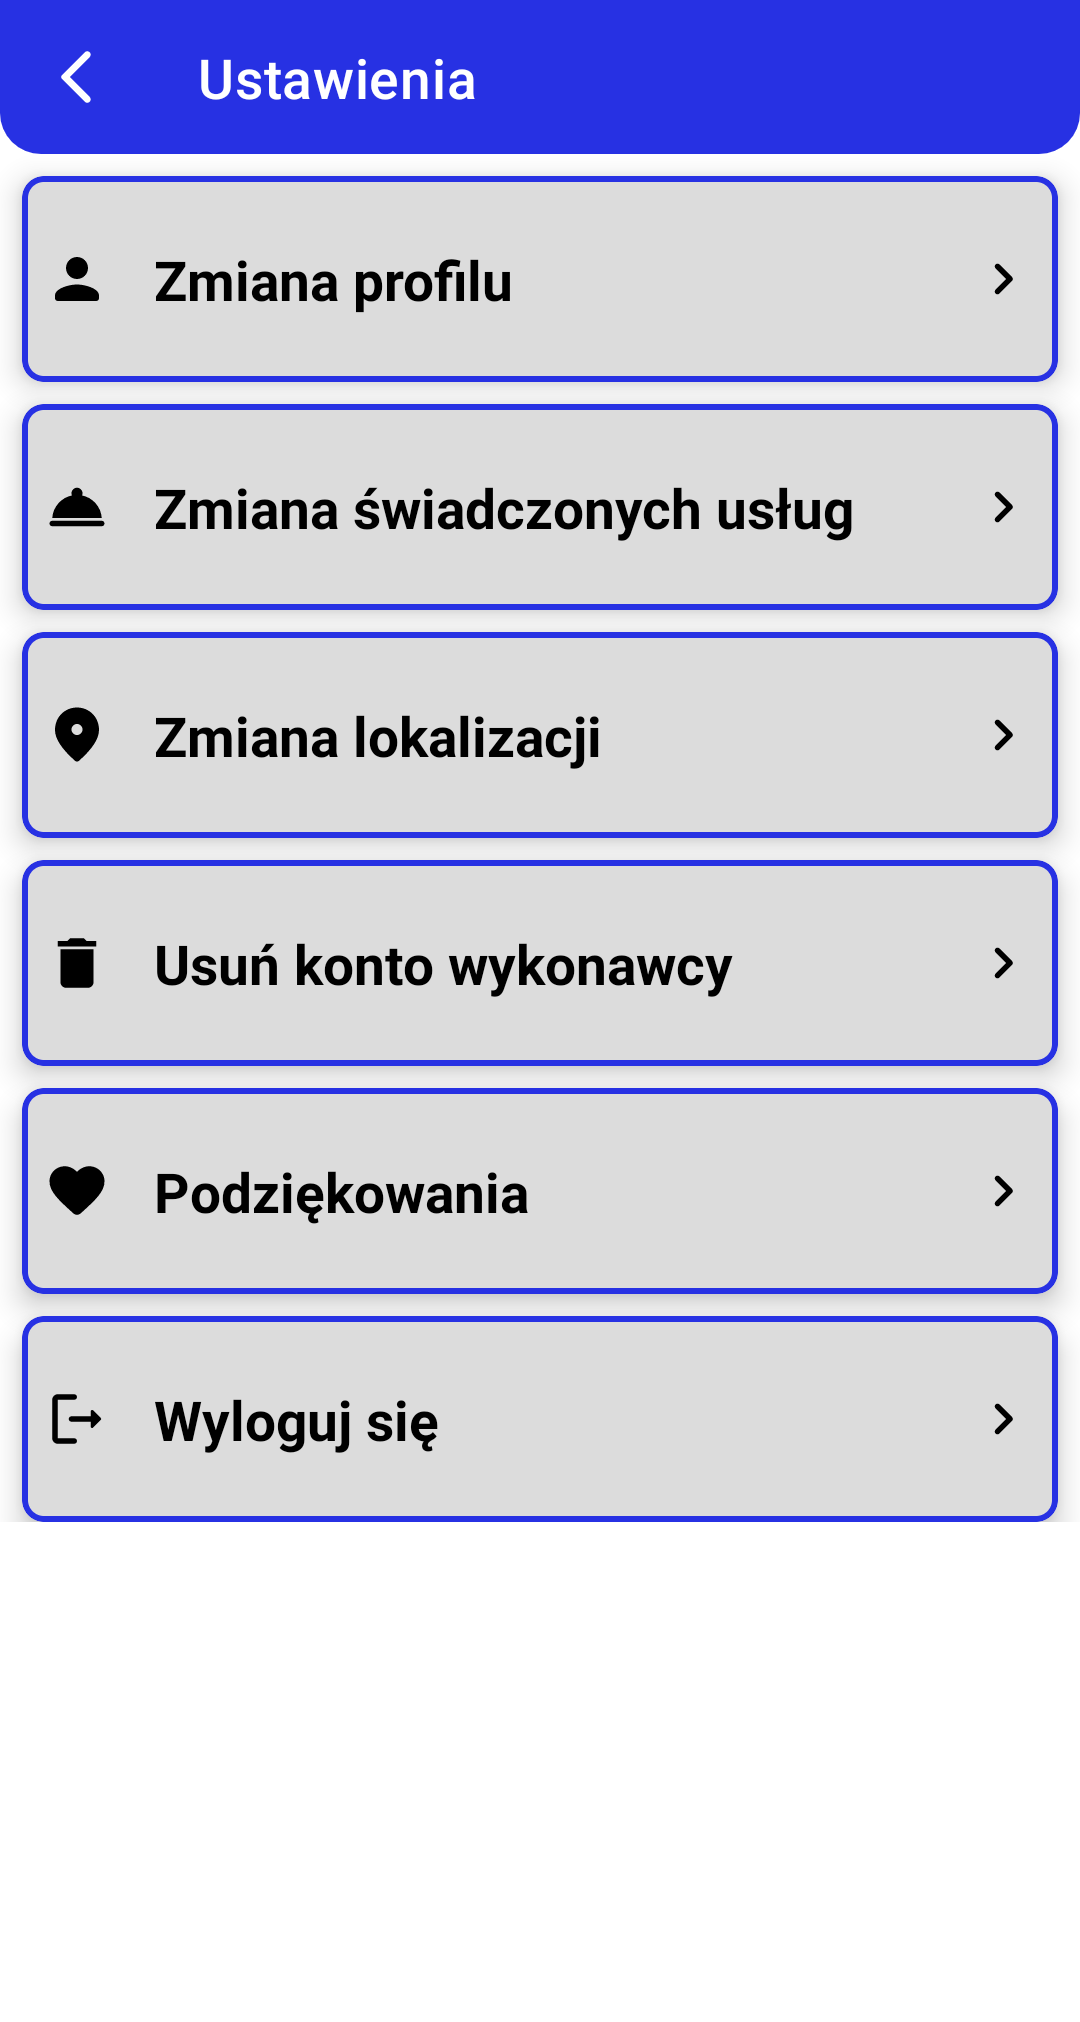
\includegraphics[width=0.97\linewidth]{screens/settings_expert.png}}
    \caption{Ekran ustawień}
  \end{subfigure}
  \begin{subfigure}{0.32\textwidth}
    \centering
    \fbox{
\includegraphics[width=0.97\linewidth]{screens/credits_expert.png}}
    \caption{Ekran podziękowań}
  \end{subfigure}
  \caption[Podstawowe ekrany]{Podstawowe ekrany w aplikacji dla wykonawców}
  \label{fig:basic-expert}
\end{figure}

Ekran powitalny, nazywany również często splash screen, jest widokiem wyświetlanym zaraz po uruchomieniu aplikacji. Została zastosowana w nim animacja, która stanowi przyjemny akcent. Podczas jej wyświetlania wykonywana jest logika określająca, który ekran powinien wyświetlić się jako kolejny. Jeżeli użytkownik nie jest zalogowany, to będzie to ekran logowania. Gdy już to zrobił, ale nie uzupełnił wszystkich wymaganych danych, to wyświetli się ekran, który to umożliwia. Jeżeli natomiast obie czynności zostały wykonane, to pokaże się ekran główny. Już tutaj widać dość skomplikowaną logikę, która dzięki wykorzystaniu trójwarstwowej architektury mogła zostać zamknięta wewnątrz przypadku użycia.

Ekran ustawień jest widokiem, którego głównym celem jest umożliwienie użytkownikom przechodzenia w inne części aplikacji. Znajdujące się w nim elementy różnią się dla wykonawców i klientów. Jedną ze wspólnych jest opcja umożliwiająca wylogowanie. Po jej wybraniu pokazywane jest okno dialogowe z prośbą o potwierdzenie.

Ekran podziękowań zawiera informacje o źródłach i autorach wykorzystanych grafik, jeśli tego wymagały. Znajdujące się tam wpisy dotyczą głównie ikon ze strony flaticon.com \cite{flaticon}, którymi postanowiono się posłużyć. W przypadku chęci ich bezpłatnego użycia podjęcie takiego działania zostało przedstawione jako konieczne.
\section{Logowanie i rejestracja}

Tworzony system wymaga identyfikacji użytkowników, więc aplikacje mobilne musiały zapewniać funkcjonalność logowania i rejestracji. 
Na rysunku \ref{fig:login} przedstawione zostały pierwsze ekrany tego procesu. Na początku nie jest określone, która dokładnie czynność jest wykonywana. Dopiero gdy użytkownik wybierze metodę uwierzytelnienia i poda swój login, to następuje sprawdzenie, czy ma on konto, czy nie i procedura od tego momentu jest kontynuowana odpowiednio jako logowanie lub rejestracja.

\begin{figure}[ht]
  \centering
  \begin{subfigure}[t]{0.33\textwidth}
    \centering
    \fbox{
\includegraphics[width=0.97\linewidth]{screens/login_start.png}}
    \caption{Ekran rozpoczęcia}
  \end{subfigure}
  \begin{subfigure}[t]{0.33\textwidth}
    \centering
    \fbox{
\includegraphics[width=0.97\linewidth]{screens/login_method.png}}
    \caption{Ekran wyboru metody}
  \end{subfigure}
  \caption{Pierwsze ekrany procesu autoryzacji}
  \label{fig:login}
\end{figure}

Wybierając metody autoryzacji sugerowano się publikacją \enquote{Investigating login features in smartphone apps} \cite{login-methods}, która analizuje związki pomiędzy dostępnymi w aplikacjach mobilnych metodami logowania, a ich popularnością. Wyciągnięto w niej wniosek, że obecność logowania społecznościowego jest jednym z czynników, który skłania użytkowników do wystawiania wyższych ocen. Wykorzystanie własnych systemów autoryzacji takiej właściwości już nie przejawia. Z tego powodu postanowiono wybrać ten rodzaj logowania, a dokładnie logowanie za pomocą Google, które z uwagi na wykorzystywaną już platformę Google Firebase okazało się proste w integracji. Kierując się jednak innym artykułem \cite{social-login}, klasyczne logowanie adresem e-mail również postanowiono wykorzystać. Wymienia on obawy dotyczące prywatności, utraty anonimowości i bezpieczeństwa jako zniechęcające ludzi do używania logowania społecznościowego. Został napisany dość dawno i przypuszcza się, że nie są one już tak bardzo powszechne, jednak wciąż spotykane.

Przy implementacji logowania i rejestracji po stronie aplikacji klienckich dominującą rolę odegrała biblioteka FirebaseUI, która dostarczyła niemalże gotowy szablon procesu autoryzacji. Po skonfigurowaniu metod logowania i wyglądu, by zapewnić spójność z resztą aplikacji, wygenerowała ona wszystkie potrzebne ekrany. Kierowała się przy tym najlepszymi znanymi praktykami. Ze względu na dużą ilość takich ekranów postanowiono nie prezentować ich wyglądu. Wykorzystują one funkcję Smart Lock w celu automatycznego logowania przy użyciu zapisanych wcześniej danych oraz obsługują kłopotliwe scenariusze, takie jak odzyskiwanie konta.

\section{Uzupełnianie danych}

W tworzonym systemie założono, że powinny istnieć pewne informacje, które dla klientów i wykonawców zawsze są określone. Przykładem tego jest imię i nazwisko. Użytkownik, który ich nie określił, nie powinien być dopuszczony do głównych funkcjonalności aplikacji. Dla wykonawców wśród takich obligatoryjnych elementów znajduję się również obszar działania oraz przynajmniej jedna świadczona usługa. Bez tego nie mogliby otrzymywać żadnych zleceń i byliby nieprzydatni.

W celu żądania uzupełnienia danych stworzone zostały ekrany, które przedstawiono na rysunku \ref{fig:setup}. Są one wyświetlane po rejestracji i uniemożliwiają użytkownikom przejście dalej tak długo, jak niezbędne informacje nie są kompletne. Gdy zostaną już podane, to nie ma możliwości ich usunięcia, a dostępna jest jedynie aktualizacja. Jeśli wykorzystywane jest logowanie za pomocą Google, to imię i nazwisko zostaje automatyczne przepisane z profilu na tej platformie i danych do uzupełnienia jest mniej.

\begin{figure}[ht]
  \centering
  \begin{subfigure}[t]{0.33\textwidth}
    \centering
    \fbox{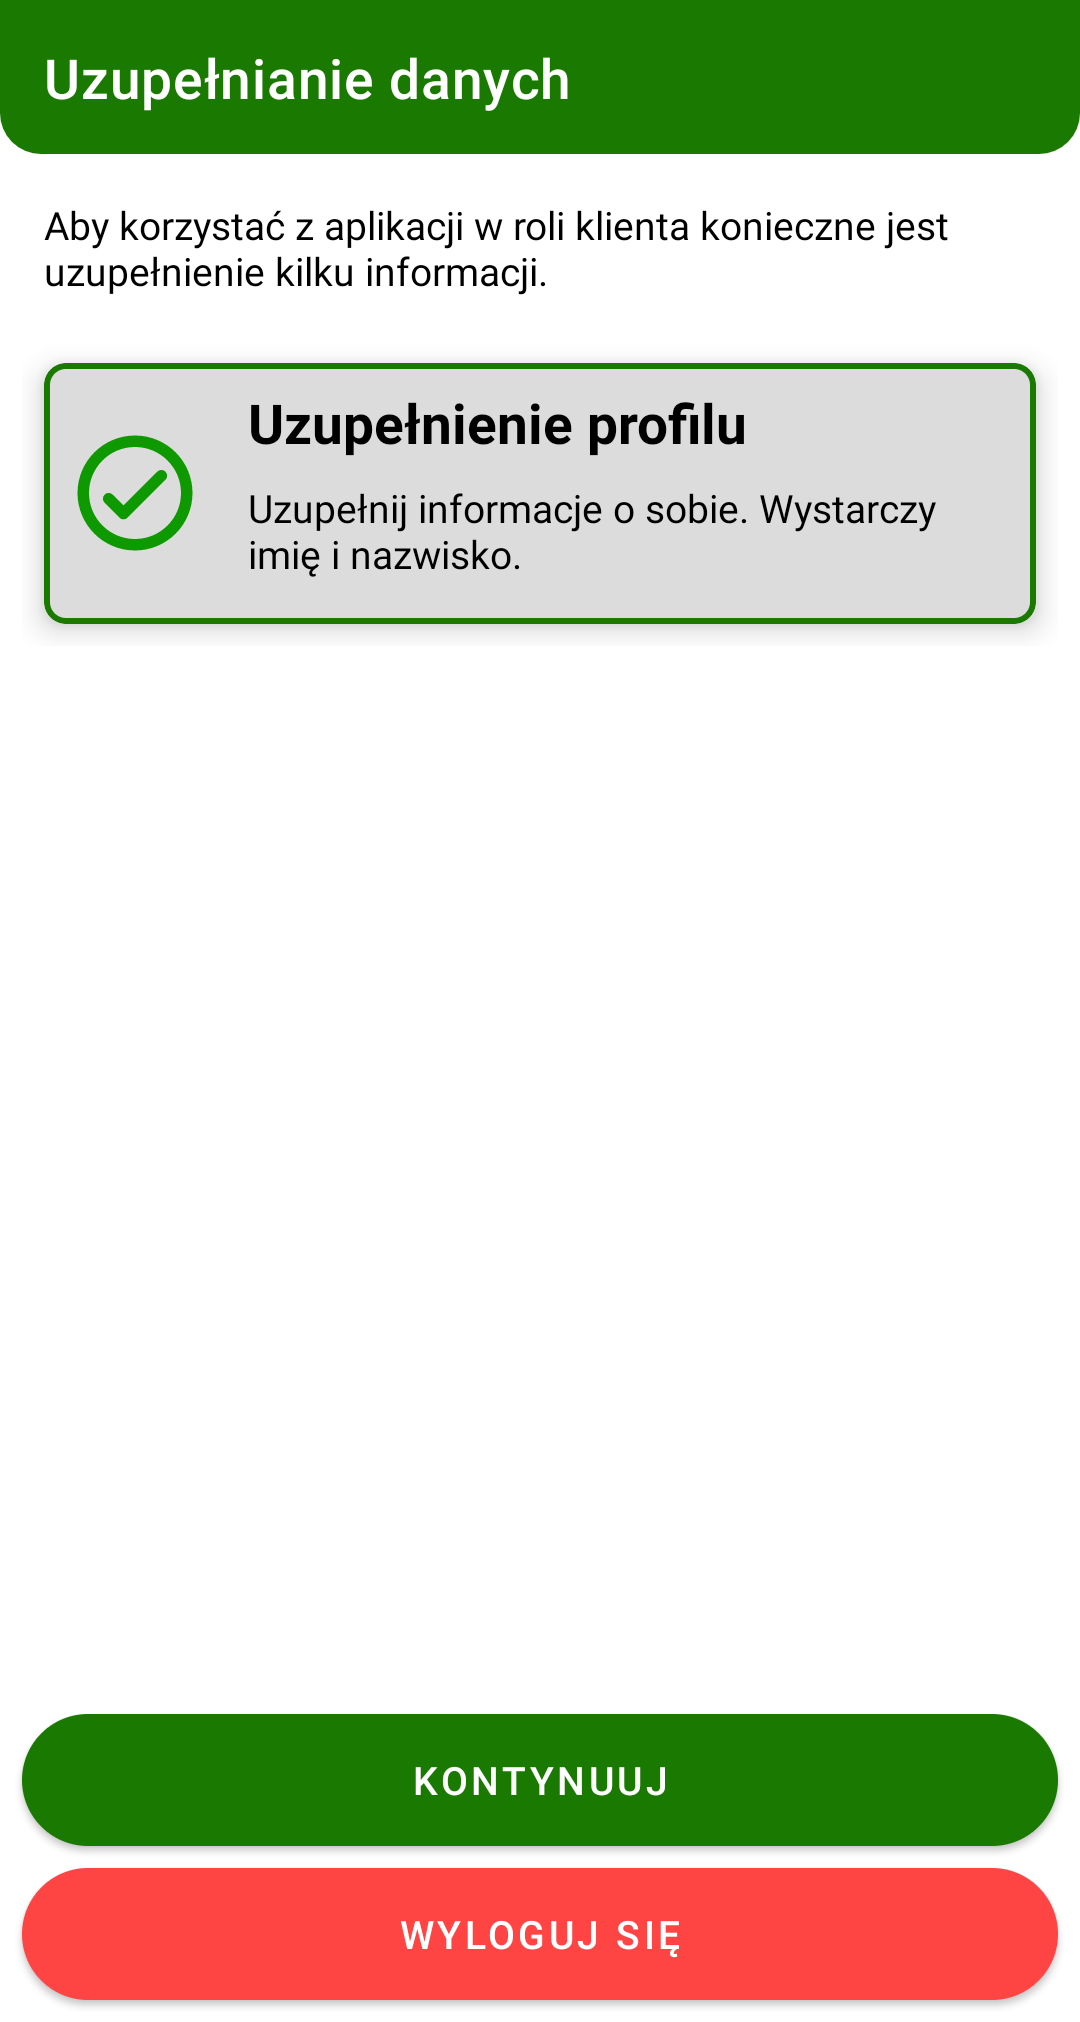
\includegraphics[width=0.97\linewidth]{screens/setup_client.png}}
    \caption{Widok klientów}
  \end{subfigure}
  \begin{subfigure}[t]{0.33\textwidth}
    \centering
    \fbox{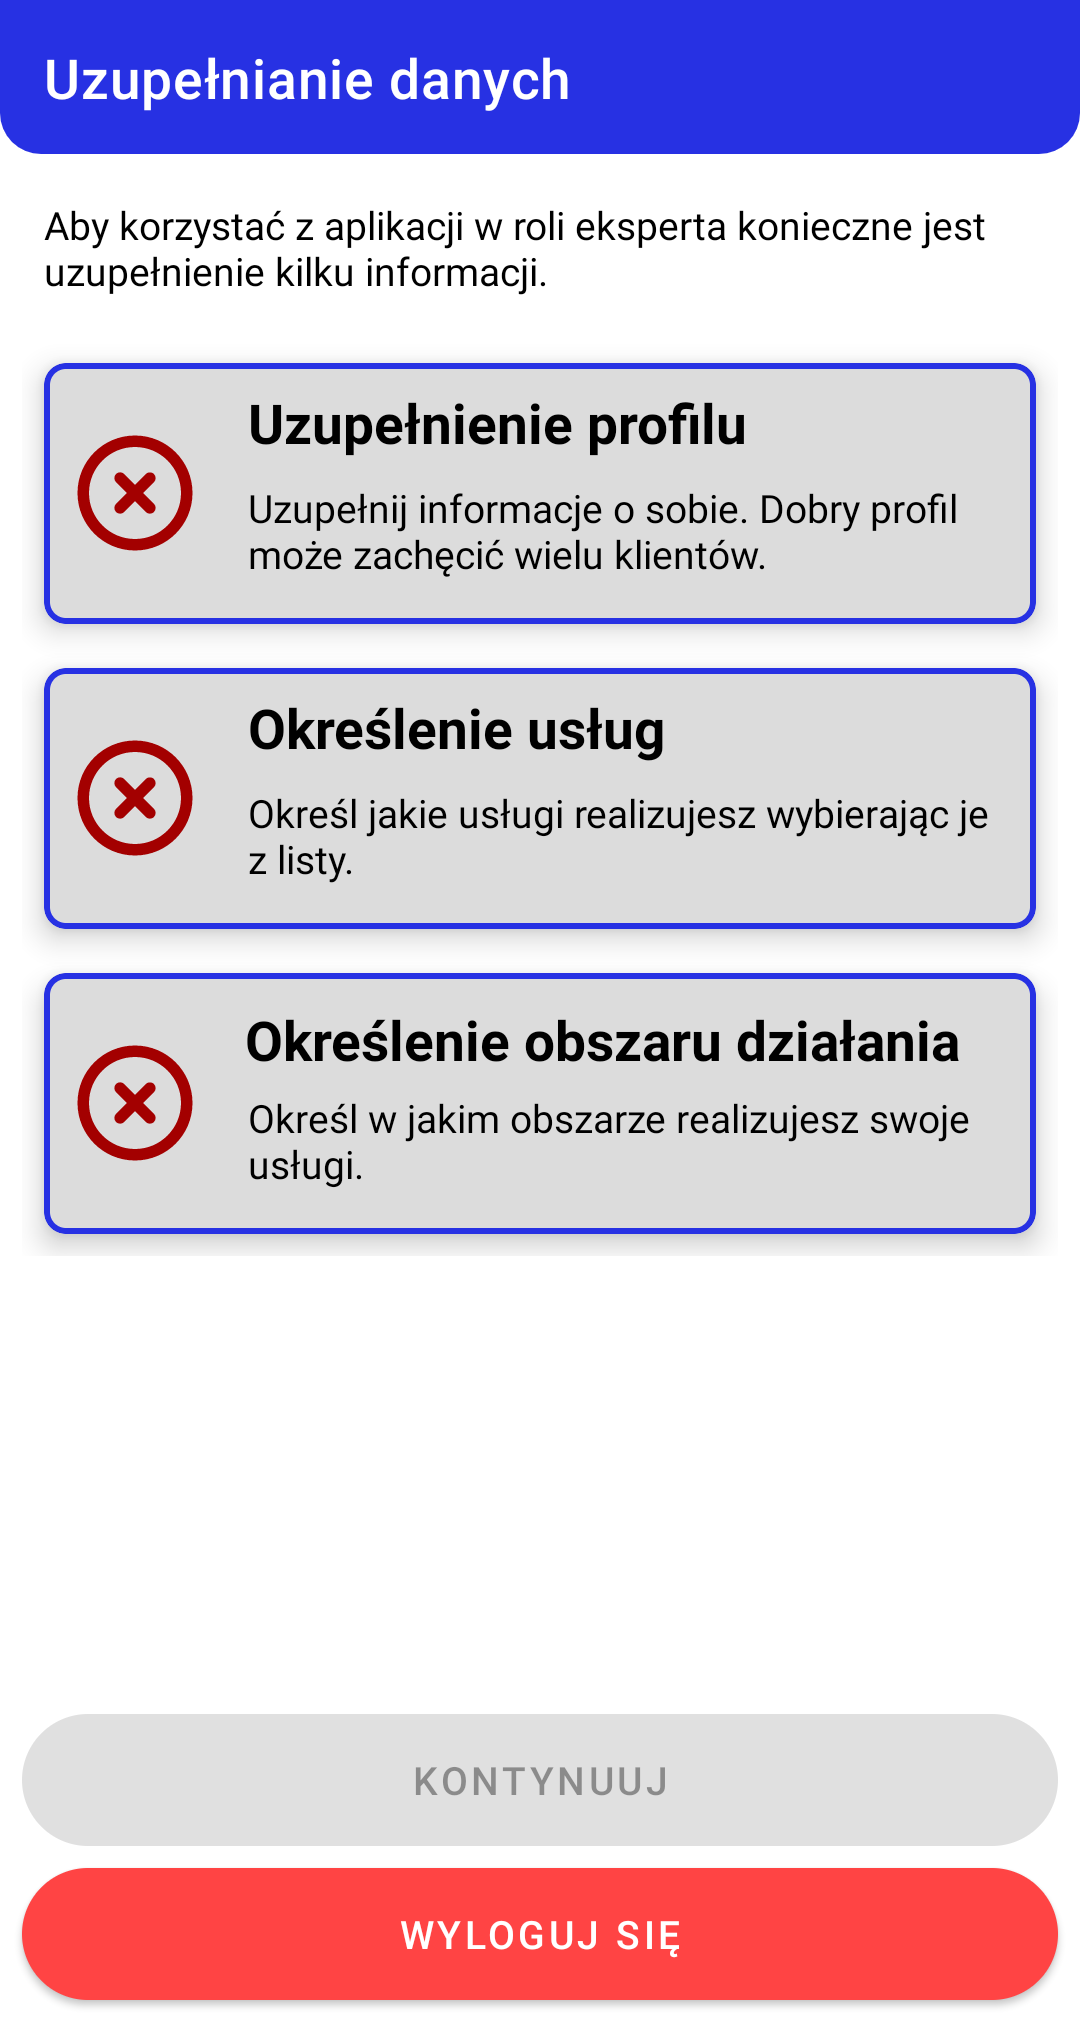
\includegraphics[width=0.97\linewidth]{screens/setup_expert.png}}
    \caption{Widok wykonawców}
  \end{subfigure}
  \caption{Ekrany uzupełniania danych}
  \label{fig:setup}
\end{figure}

Ekrany uzupełniania danych składają się z listy kart, z których każda zawiera informację o akcji koniecznej do podjęcia. Obok nich są również umieszczone ikonki, które mówią, czy zostały już wykonane. Można tego dokonać poprzez wybranie karty, co spowoduje przeniesienie do części aplikacji, która umożliwia modyfikację koniecznych danych. Po ich zatwierdzeniu nastąpi powrót i przy odpowiedniej karcie ikonka krzyżyka zmieni się na ikonkę ptaszka, mówiąc o powodzeniu operacji. Gdy użytkownik spełni wszystkie warunki, to przycisk kontynuacji stanie się aktywny i umożliwi przejście do ekranów głównych. Gdyby jednak nie chciał z jakichś powodów tego zrobić, lecz się wylogować, to również dano mu taką możliwość za pomocą przewidzianego do tego celu przycisku. 
\section{Zmiana profilu}

Zmiana profilu to funkcjonalność umożliwiająca użytkownikom edycję podstawowych informacje na swój temat. Ma ona szczególne znaczenie i jest bardziej rozbudowana w przypadku wykonawców. Powodem jest to, że ustalane informacje są widoczne dla klientów i w ten sposób mogą wpłynąć na podejmowane przez nich wybory.

\begin{figure}[ht]
  \centering
  \begin{subfigure}[t]{0.33\textwidth}
    \centering
    \fbox{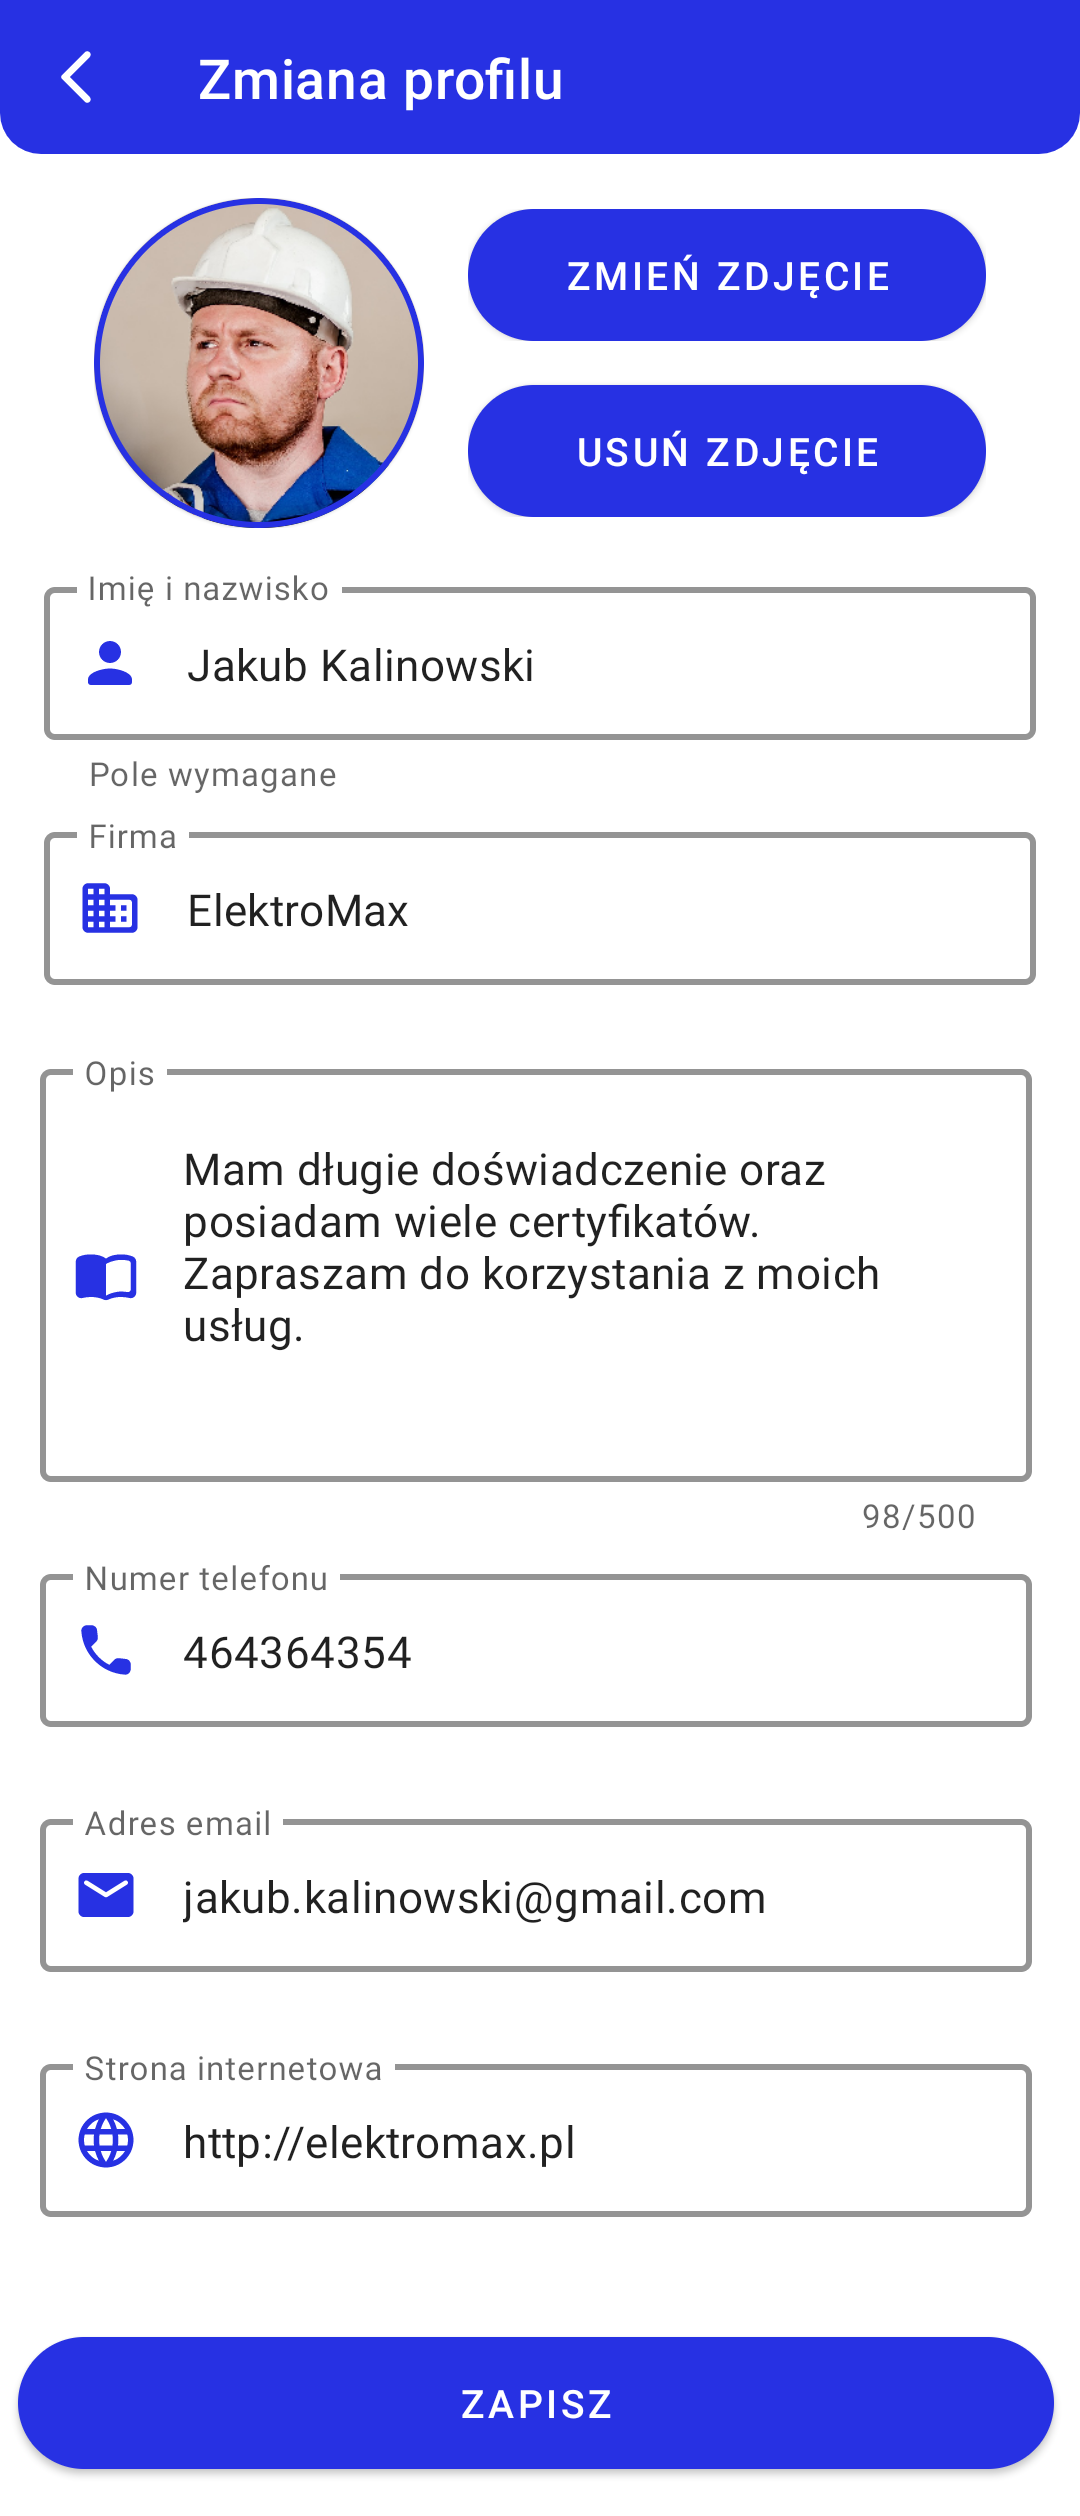
\includegraphics[width=0.97\linewidth]{screens/info_expert.png}}
    \caption{Widok wykonawców}
  \end{subfigure}
  \begin{subfigure}[t]{0.33\textwidth}
    \centering
    \fbox{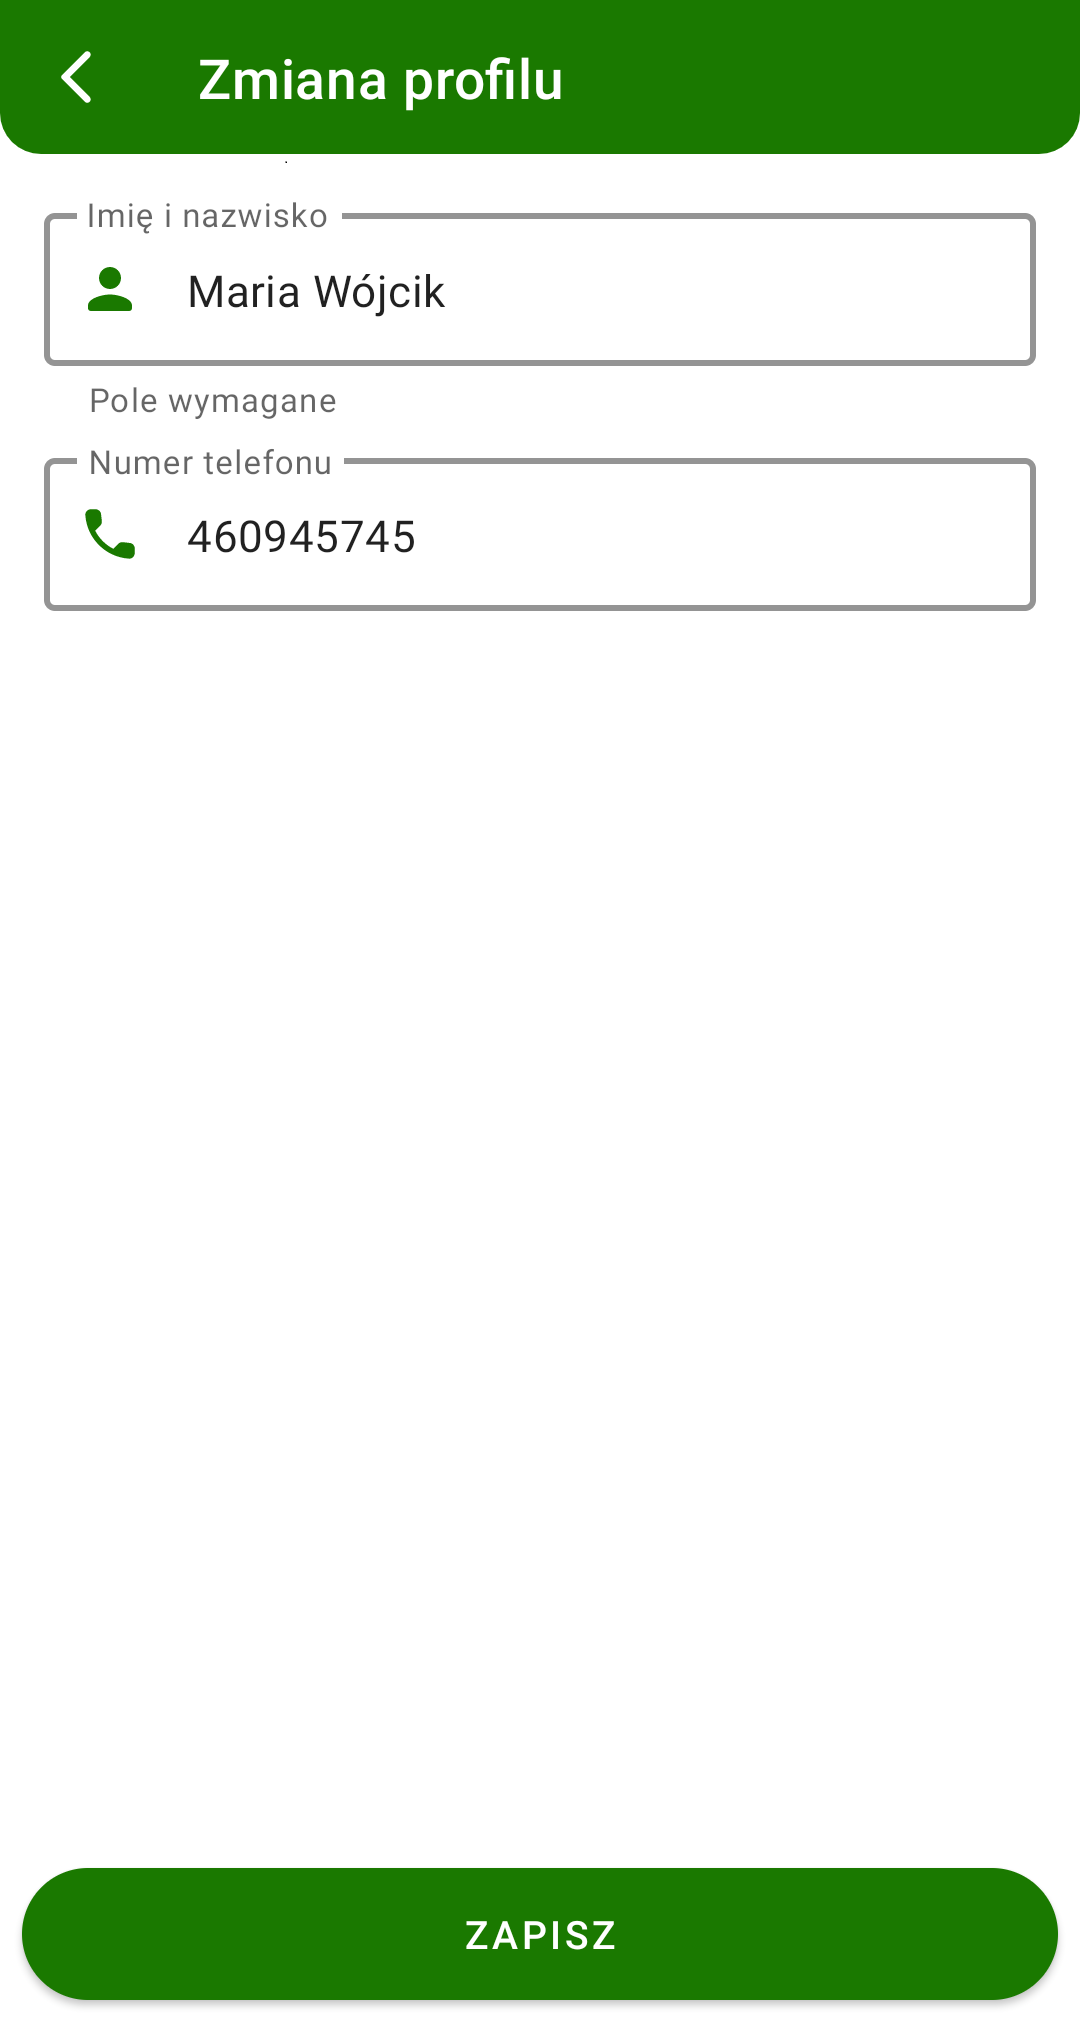
\includegraphics[width=0.97\linewidth]{screens/info_client.png}}
    \caption{Widok klientów}
  \end{subfigure}
  \caption{Ekran zmiany profilu}
  \label{fig:info-expert}
\end{figure}

Na rysunku \ref{fig:info-expert} przedstawione zostały ekrany zmiany profilu dla obu aplikacji. Jedynym elementem obligatoryjnym, który musi być na nich wypełniony, jest imię i nazwisko. Bez tego przycisk zapisu nie stanie się aktywny. Pozostałe pola są opcjonalne, lecz jeżeli zostaną wypełnione, a znajdujące się w nich dane nie będą poprawne, to przycisku zapisu również nie będzie można użyć. Wszystkie wartości są walidowane, a ewentualne informacje o błędach wyświetlane obok. Zostały wykorzystane w tym celu proste warunki, jak i wyrażenia regularne. Aplikacja dla wykonawców wyróżnia się obecnością komponentu do modyfikacji zdjęcia profilowego. Po wyrażeniu chęci jego zmiany na inne ukazuje się ekran służący do wyboru obrazu, a następnie przycięcia w kształt koła.

W kontekście zdjęć profilowych wykorzystany został interesujący mechanizm, aby zmniejszyć częstość ich pobierania. Jest to niepożądane z uwagi na generowany ruch sieciowy oraz koszty. Zdjęcia są oczywiście cachowane przez aplikacje klienckie, lecz jeśli byłyby wciąż wyciągane z pamięci podręcznej, to ich aktualizacje nie byłyby zauważane. Z tego powodu w bazie danych przechowywane są daty ostatnich ich modyfikacji. Dzięki temu możliwe jest ponowne pobranie zdjęcia profilowego jedynie wtedy, gdy zostanie zauważone, że ostatnia data jego modyfikacji została zmieniona na nowszą. Ogranicza to częstość pobierania zdjęć profilowych do minimum.

% Informacje widoczne na ekranach pobierane są bezpośrednio z bazy Firebase Firestore. Zapis wartości z pól tekstowych dokonywany jest natomiast poprzez jawnie wywoływaną funkcję Firebase Functions. Umożliwia ona przeprowadzenie walidacji danych w bezpiecznym środowisku przed ich utrwaleniem. Dodawanie, zmienianie oraz usuwanie zdjęć profilowych dokonuje się natomiast poprzez wykonywanie odpowiednich operacji na magazynie plików Firebase Storage.
\section{Zmiana świadczonych usług}

Zmiana świadczonych usług to ważna z punktu widzenia wykonawcy funkcjonalność. Zapewnia ograniczenie przydzielanych mu zleceń jedynie do tych, których realizacją może być zainteresowany. Rysunek \ref{fig:services} jest zrzutem ekranu, który ją prezentuje.
Sam wybór usług jest dokonywany poprzez zaznaczenie na liście. W celu lepszej organizacji i zwiększenia przejrzystości zostały one pogrupowane w kategorie, z których w danej chwili tylko jedna może być rozwinięta. Wymaga się, aby wykonawca świadczył przynajmniej jedną usługę. Jeżeli takowa nie jest określona, to wyświetlany jest komunikat mówiący o konieczności jej wybrania.

\begin{figure}[ht!]
  \centering
  \fbox{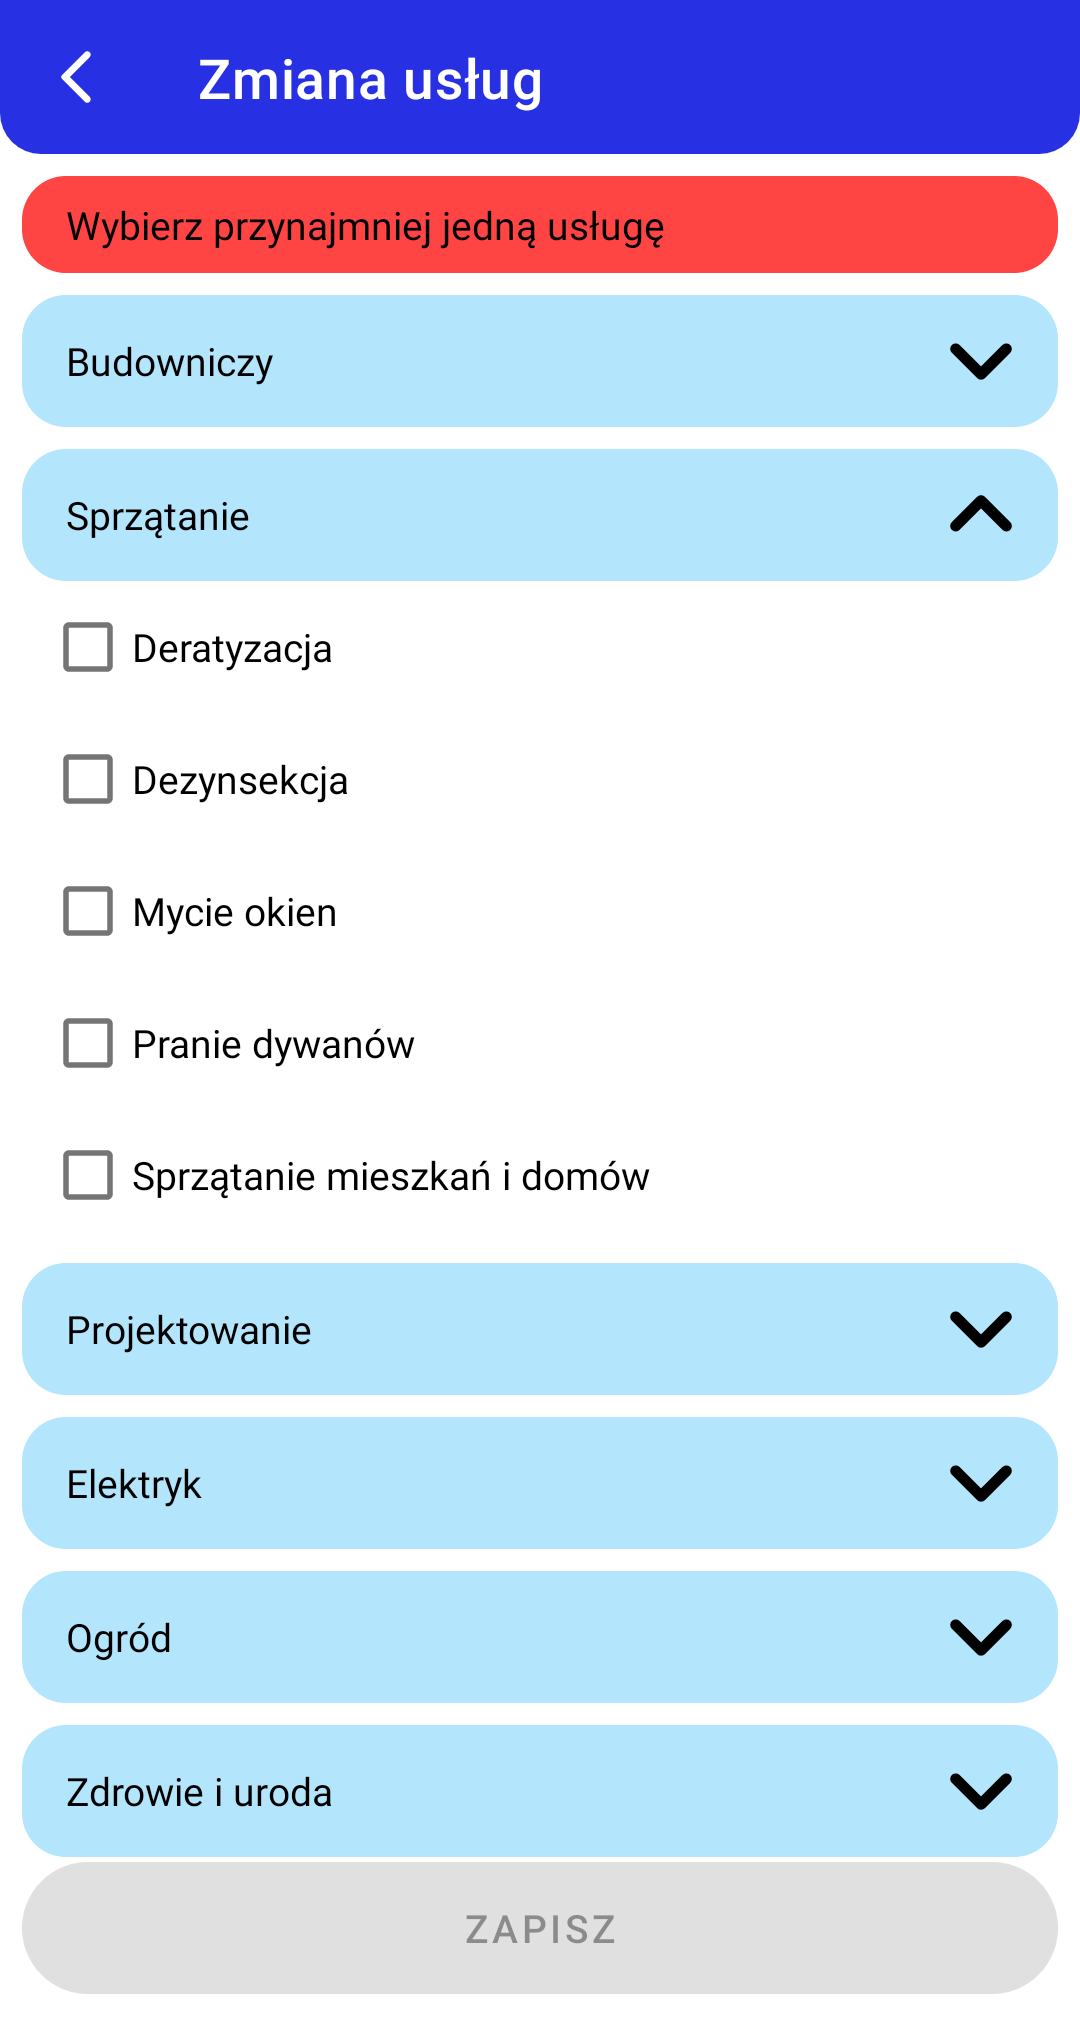
\includegraphics[width=0.33\linewidth]{screens/services.png}}
  \caption{Ekran zmiany świadczonych usług}
  \label{fig:services}
\end{figure}

\section{Zmiana obszaru działania}

Zmiana obszaru działania to kolejna funkcjonalność umożliwiająca doprecyzowanie zleceń, które wykonawcy mają dostawać. Obszar ten zapewnia ograniczenie przydzielanych zleceń jedynie do tych, których realizacja ma się odbyć wewnątrz niego. Pozwala to odfiltrować te, które nie mogą zostać wykonane z uwagi na zbyt duże odległości. 

\pagebreak

% W stworzonym rozwiązaniu przyjęto, że obszar działania jest kołem. Powodem tego jest możliwość jego prostego zdefiniowania. Wystarczą do tego jedynie dwa parametry: centralna lokalizacja oraz promień.

Przyjęcie obszaru działania w postaci koła wymagało decyzji, czy jego promień ma być ograniczony górną granicą. Postanowiono ją wprowadzić, ponieważ zmniejsza to negatywny wpływ, jaki mogą wywierać na system nieodpowiednio korzystające z niego osoby. Mogłyby one, będące wykonawcami, wyrazić chęć świadczenia wszystkich usług na terenie całego kraju. W ten sposób zyskają dostęp do wszystkich zleceń i możliwość zgłaszania się do nich. Problem pojawia się, gdy zaczną to robić bez chęci realizacji. Aby temu zjawisku przeciwdziałać, maksymalny promień obszaru działania ograniczono do 50 kilometrów. Uznano, że jest to wartość wystarczająca dla zdecydowanej liczby prawidłowo używających systemu wykonawców.

% W tworzonym rozwiązaniu założono, że wykonawcy będą otrzymywać jedynie te zlecenia, których wykonanie ma się odbyć w obrębie określonego przez nich wcześniej obszaru działania. Postanowiono również, że wspomniany obszar działania będzie kołem, które można określić przy pomocy centralnej lokalizacji oraz promienia.

\begin{figure}[ht]
  \captionsetup[subfigure]{justification=centering}
  \centering
  \begin{subfigure}{0.32\textwidth}
    \centering
    \fbox{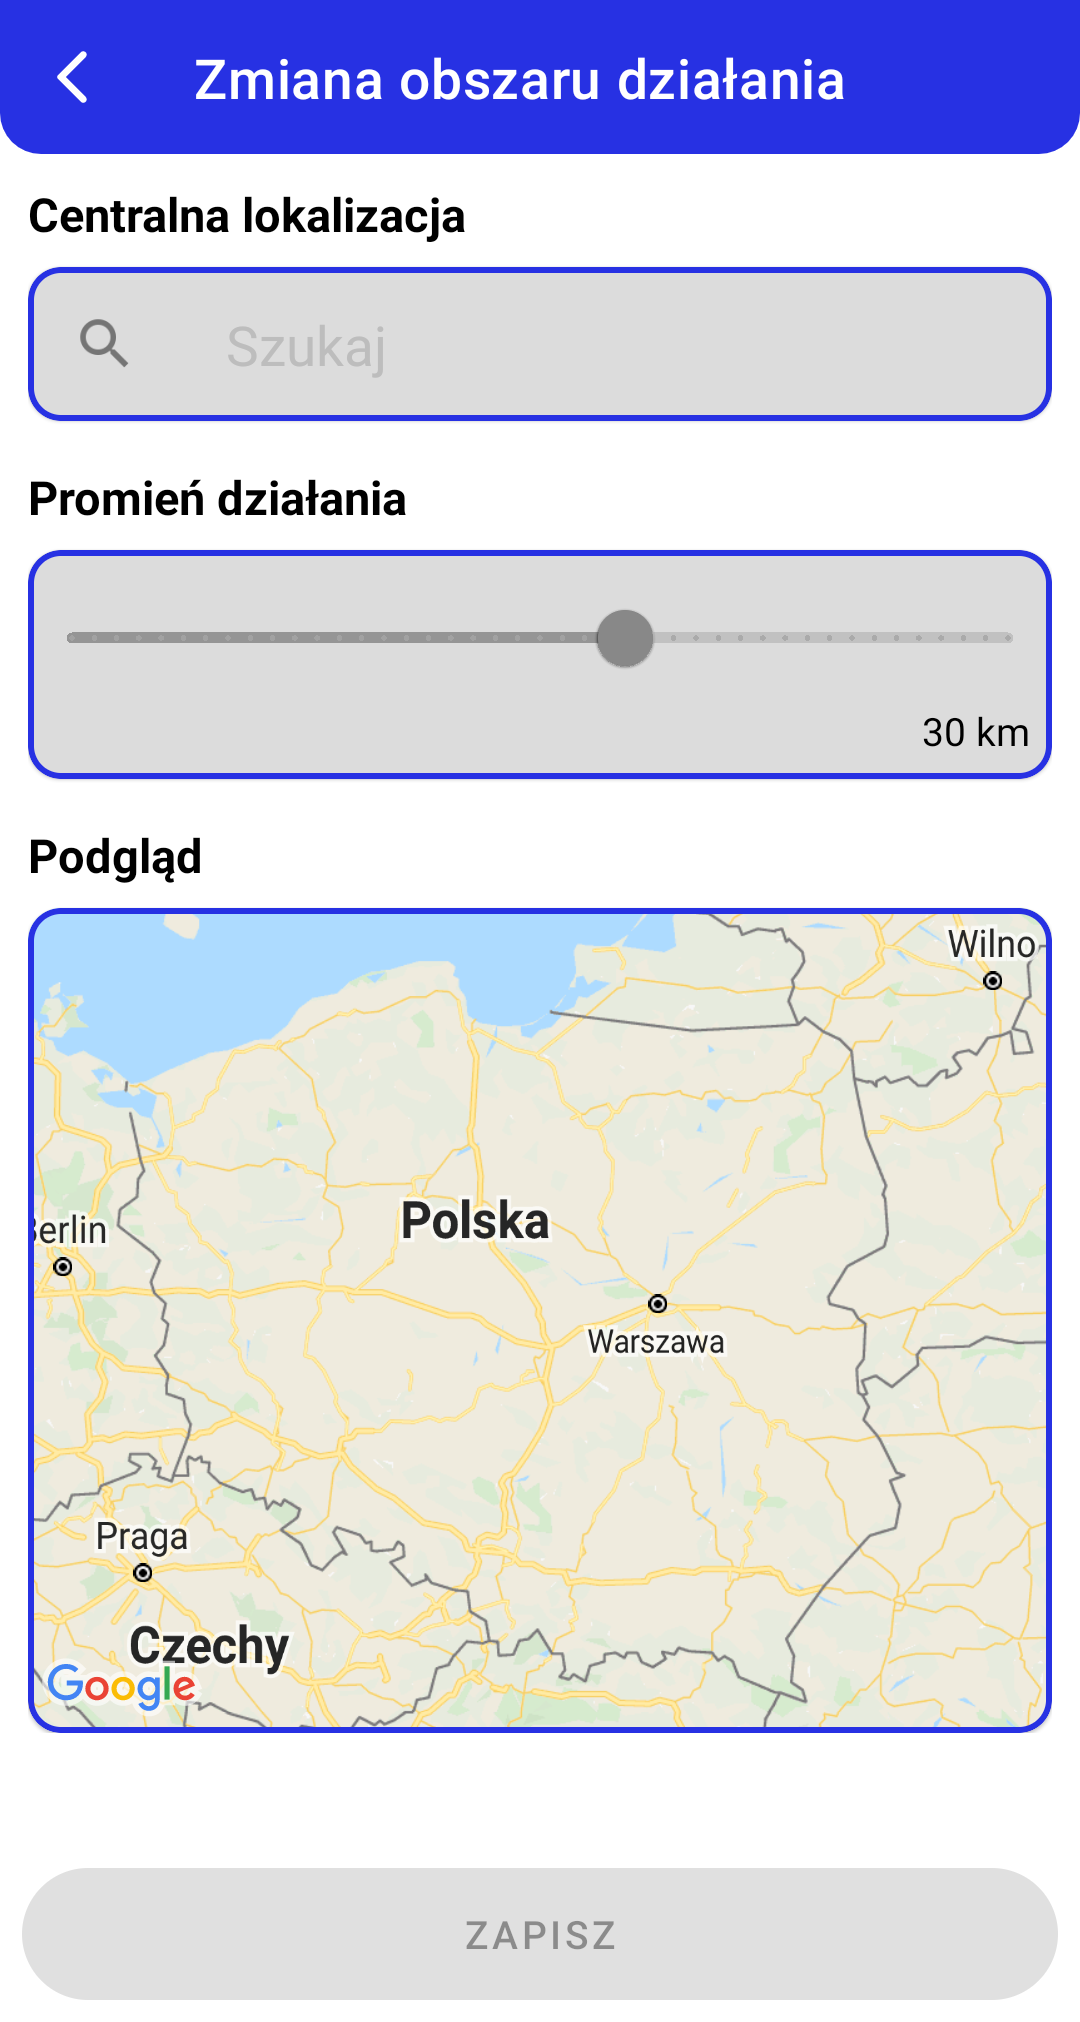
\includegraphics[width=0.97\linewidth]{screens/location_empty.png}}
    \caption{Widok nieokreślonego obszaru działania}
  \end{subfigure}
  \begin{subfigure}{0.32\textwidth}
    \centering
    \fbox{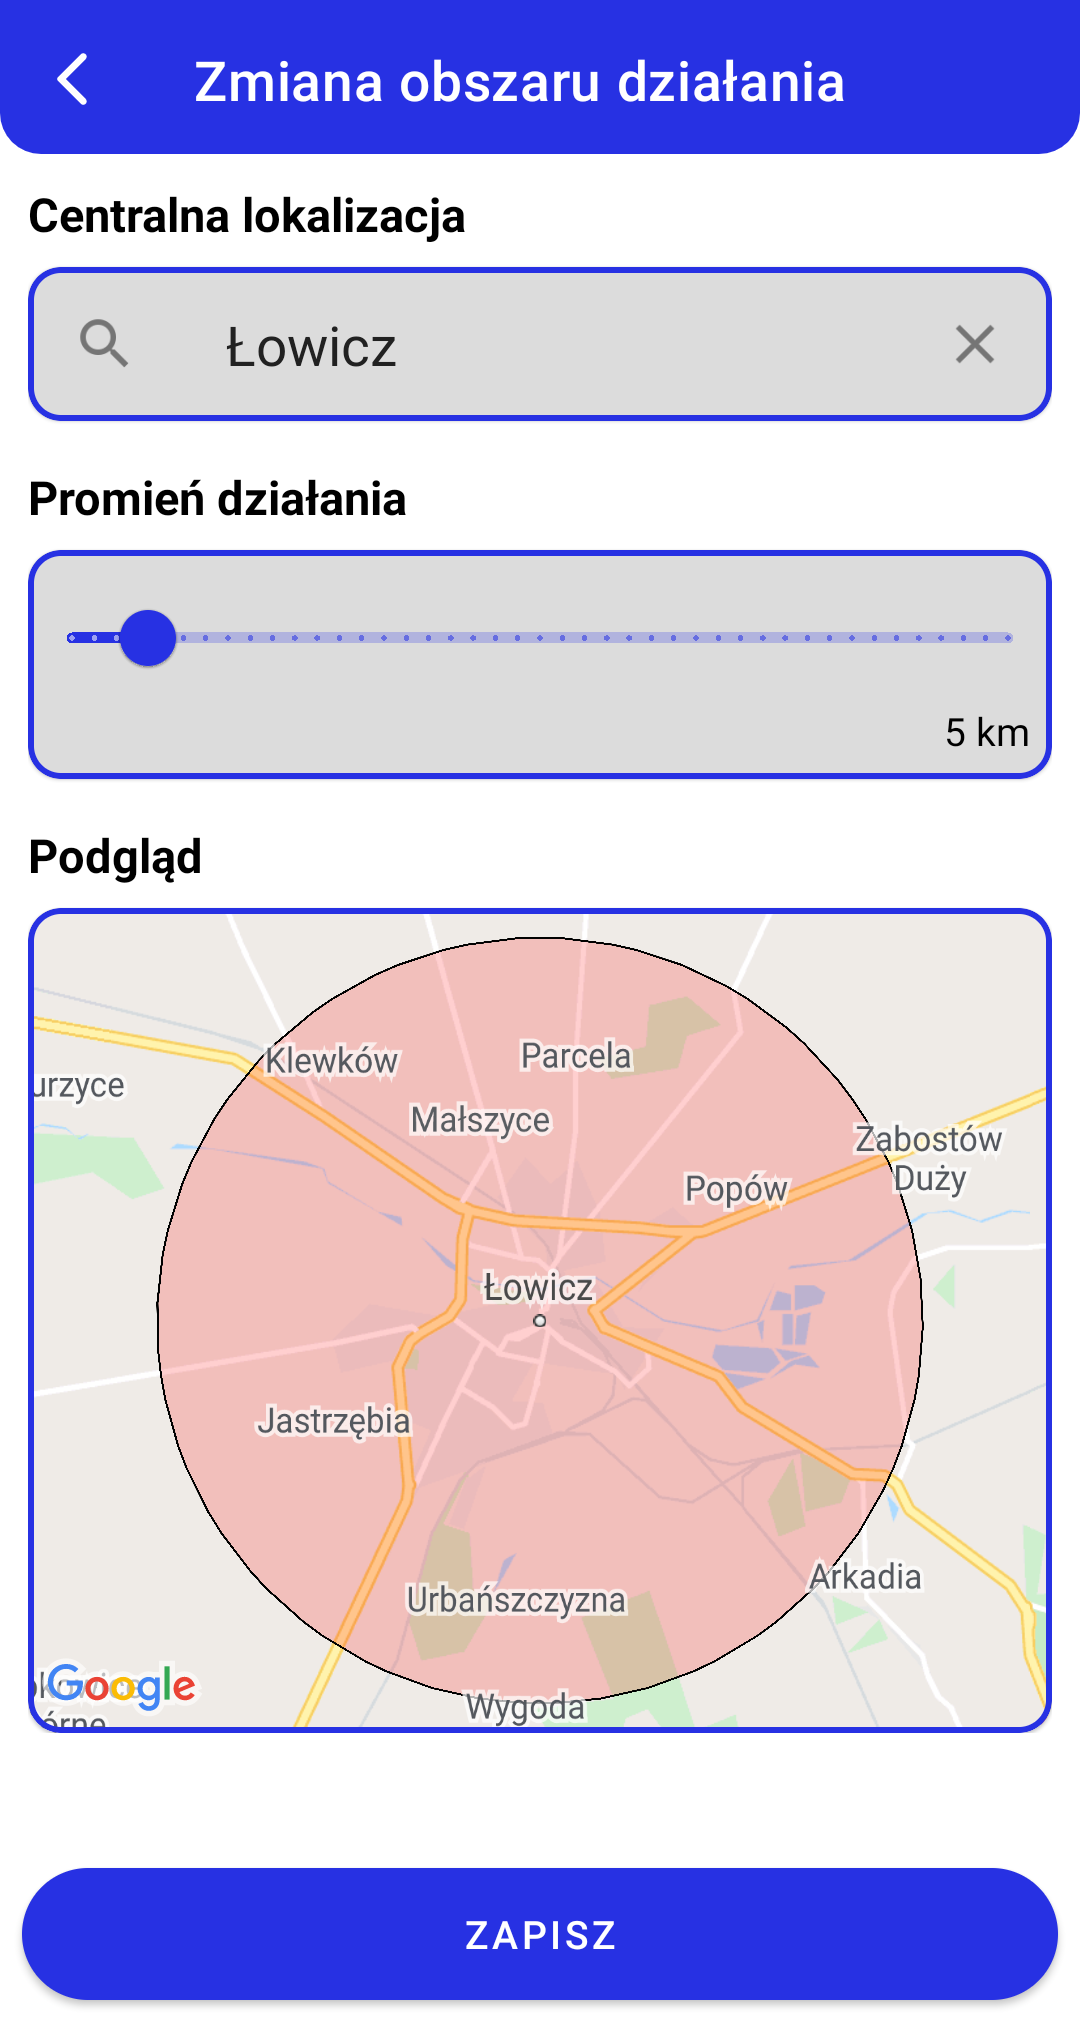
\includegraphics[width=0.97\linewidth]{screens/location_filled.png}}
    \caption{Widok określonego obszaru działania}
  \end{subfigure}
  \begin{subfigure}{0.32\textwidth}
    \centering
    \fbox{
\includegraphics[width=0.97\linewidth]{screens/location_city.png}}
    \caption{Widok wyboru centralnej lokalizacji}
  \end{subfigure}
  \caption{Ekran zmiany obszaru działania}
  \label{fig:location}
\end{figure}

% Na rysunku \ref{fig:location} przedstawiony został ekran, który umożliwia zmianę lokalizacji wykonawcy. Składa się on z kontrolek umożliwiających określenie centralnej lokalizacji i promienia oraz podglądu, który te informacje wizualizuje. Wybór lokalizacji ograniczony jest do polskich miejscowości, a promienia do ustalonych 50 kilometrów.

Podczas implementacji wykorzystana została platforma Google Maps Platform i składające się na nią produkty Maps oraz Places. Umożliwiły one osadzenie mapy wewnątrz aplikacji, dostarczyły komponent wyboru lokalizacji oraz zapewniły geokodowanie, które wykorzystano wewnątrz Firebase Functions w celu walidacji poprawności lokalizacji. 
% \newpage
\section{Dodawanie nowych zleceń}

Dodawanie nowych zleceń jest jedną z głównych funkcjonalności, która jest specyficzna dla klientów. Z tego powodu została umieszczona w ich aplikacji. Składa się na nią aż pięć ekranów, które przedstawiono na rysunku \ref{fig:add-job}. Każdy z nich stanowi inny etap procesu tworzenia zlecenia. Poruszanie pomiędzy nimi odbywa się sekwencyjnie - aby dostać się do danego ekranu trzeba przejść przez wszystkie wcześniejsze. 

Dodawanie zlecenia rozpoczyna się od zakładki \enquote{dodaj zlecenie} znajdującej się na ekranie głównym aplikacji dla klientów. Zawiera listę wszystkich dostępnych kategorii. Po wybraniu jednej z nich użytkownik zostaje przeniesiony do ekranu, który przedstawia podobną listę, lecz zawierającą usługi, które należą do wybranej chwilę wcześniej kategorii. Od tego momentu widoczny jest pasek postępu, który informuje o aktualnym etapie tworzenia zlecenia. Gdy usługa również zostanie wybrana, to bieżący widok zmienia się w ekran wyboru lokalizacji. Przy jego pomocy określane jest miejsce, w którym usługa ma być świadczona. Miejscowość można wpisać przy pomocy przeznaczonego do tego pola, które zapewnia automatyczne uzupełnienie. Spodziewano się jednak, że klienci często będą korzystali z tych samych lokalizacji. Może nią być na przykład miejsca zamieszkania. Z tego powodu przewidziano funkcję zapamiętywania tych ostatnio wprowadzonych i możliwość ich szybkiego wyboru z listy. Przenosi on użytkownika do ekranu uzupełnienia szczegółów. W przeznaczonym na to miejscu klienci mogą przedstawić szczegóły usługi, której wykonania wymagają, a w polu czasu realizacji określają żądany termin wykonania. Zamiast pola tekstowego rozważano możliwość wprowadzania tej informacji w sposób bardziej ścisły, na przykład poprzez wybranie konkretnych dni i godzin. Uznano jednak to rozwiązanie za zbyt ograniczające. W przypadku wartości tekstowej można bowiem użyć zwrotów bardziej ogólnych, takich jak: \enquote{jak najczybciej}, czy też \enquote{najlepiej przed}. Po uzupełnieniu obu pól i zatwierdzeniu zlecenie o podanych parametrach jest tworzone, a użytkownik zostaje o tym powiadomiony.

\begin{figure}[htp!]
  \captionsetup[subfigure]{justification=centering}
  \centering
  \begin{subfigure}[t]{0.32\textwidth}
    \centering
    \fbox{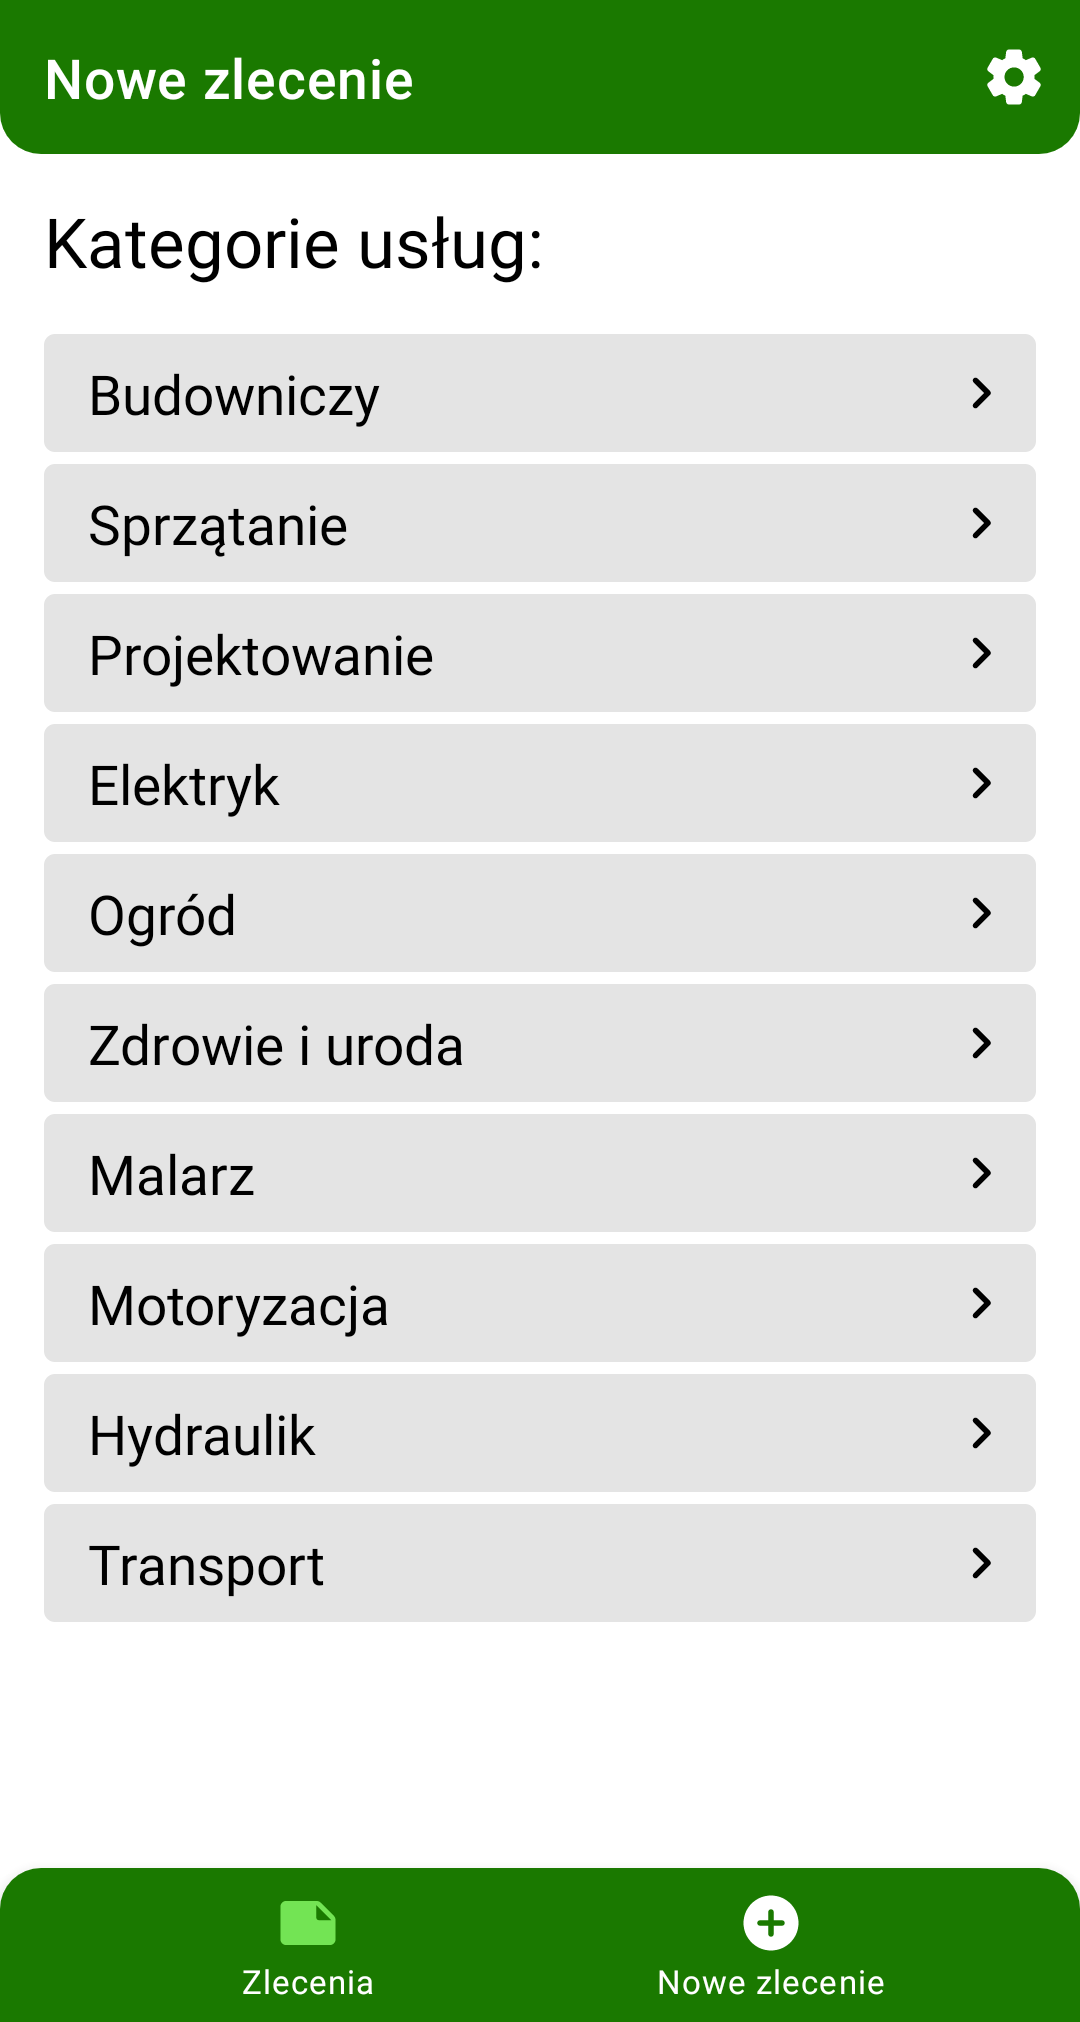
\includegraphics[width=0.97\linewidth]{screens/add_job_category.png}}
    \caption{Ekran wyboru kategorii}
  \end{subfigure}
  \begin{subfigure}[t]{0.32\textwidth}
    \centering
    \fbox{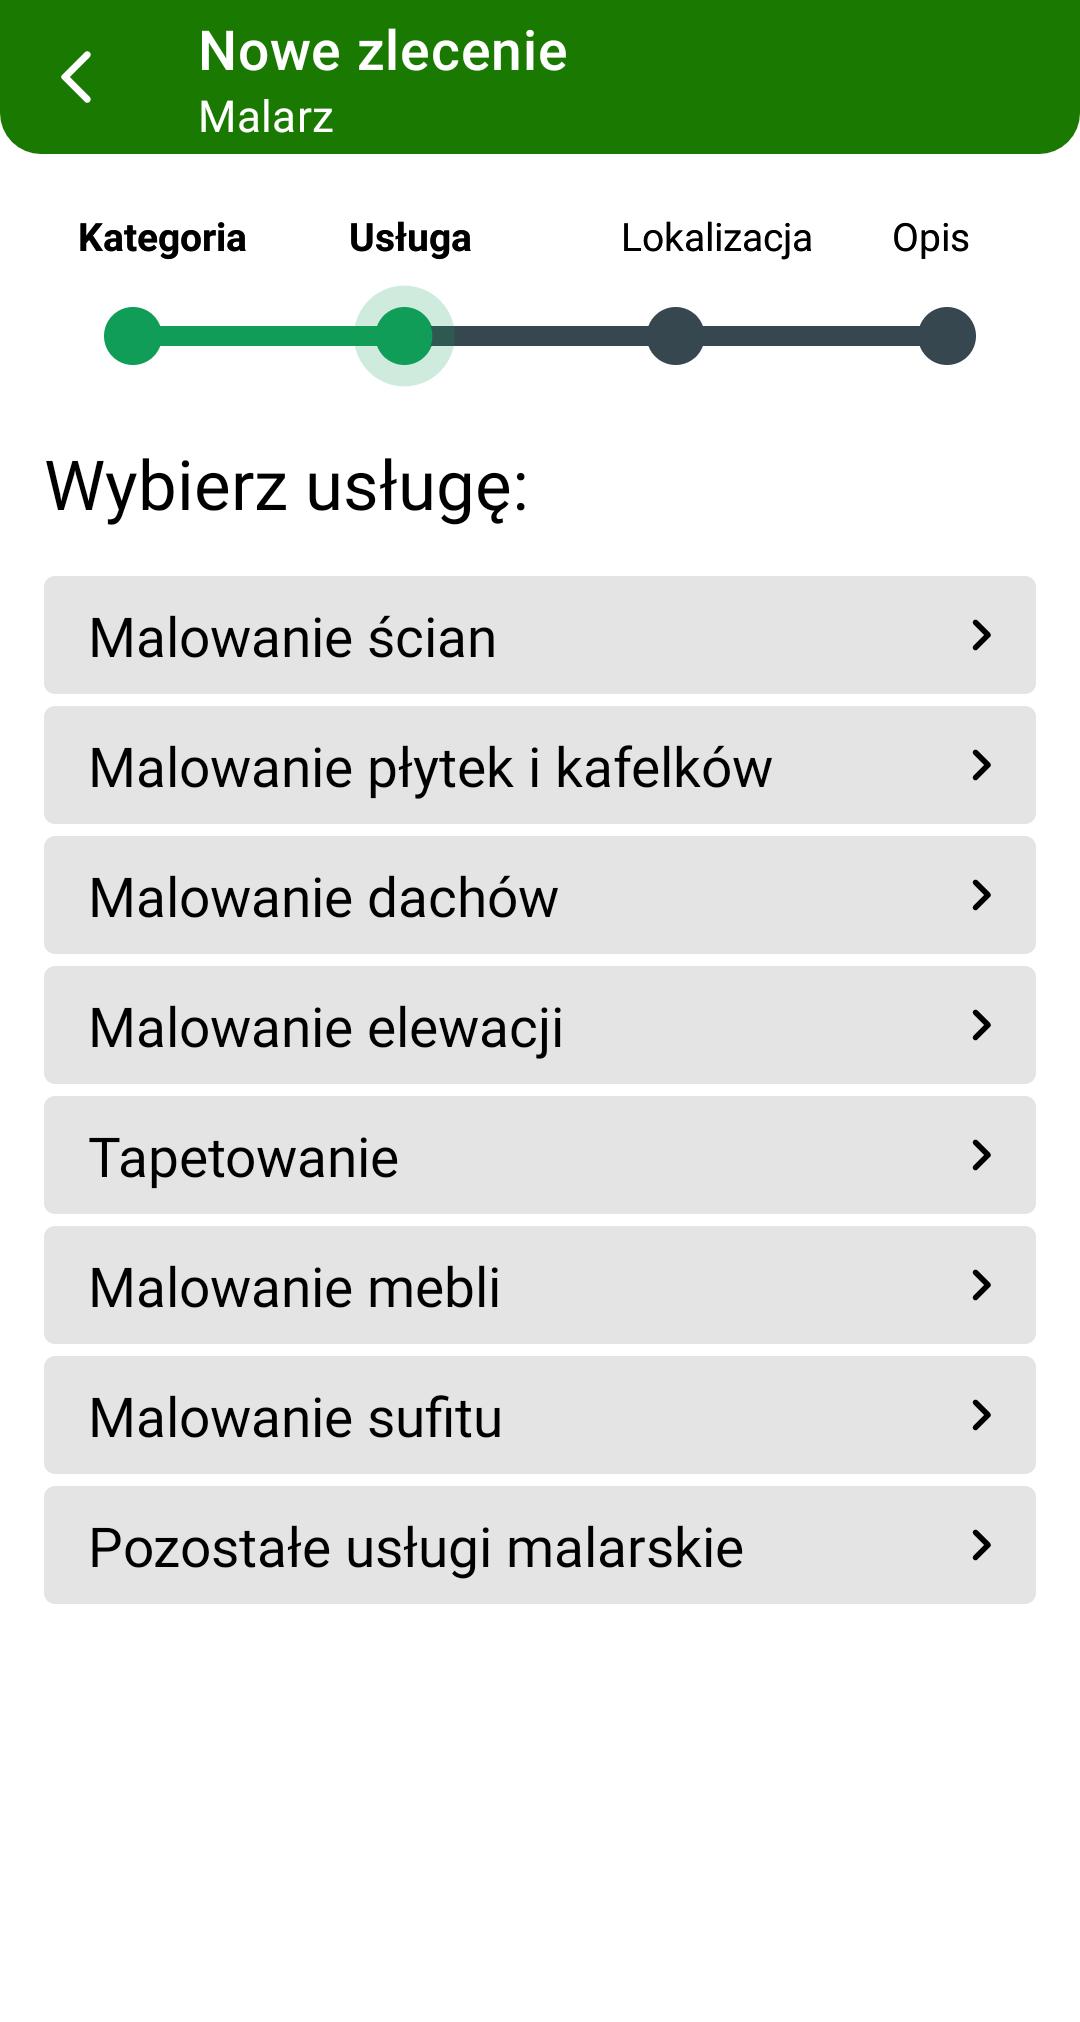
\includegraphics[width=0.97\linewidth]{screens/add_job_service.png}}
    \caption{Ekran wyboru usługi}
  \end{subfigure}
  \begin{subfigure}[t]{0.32\textwidth}
    \centering
    \fbox{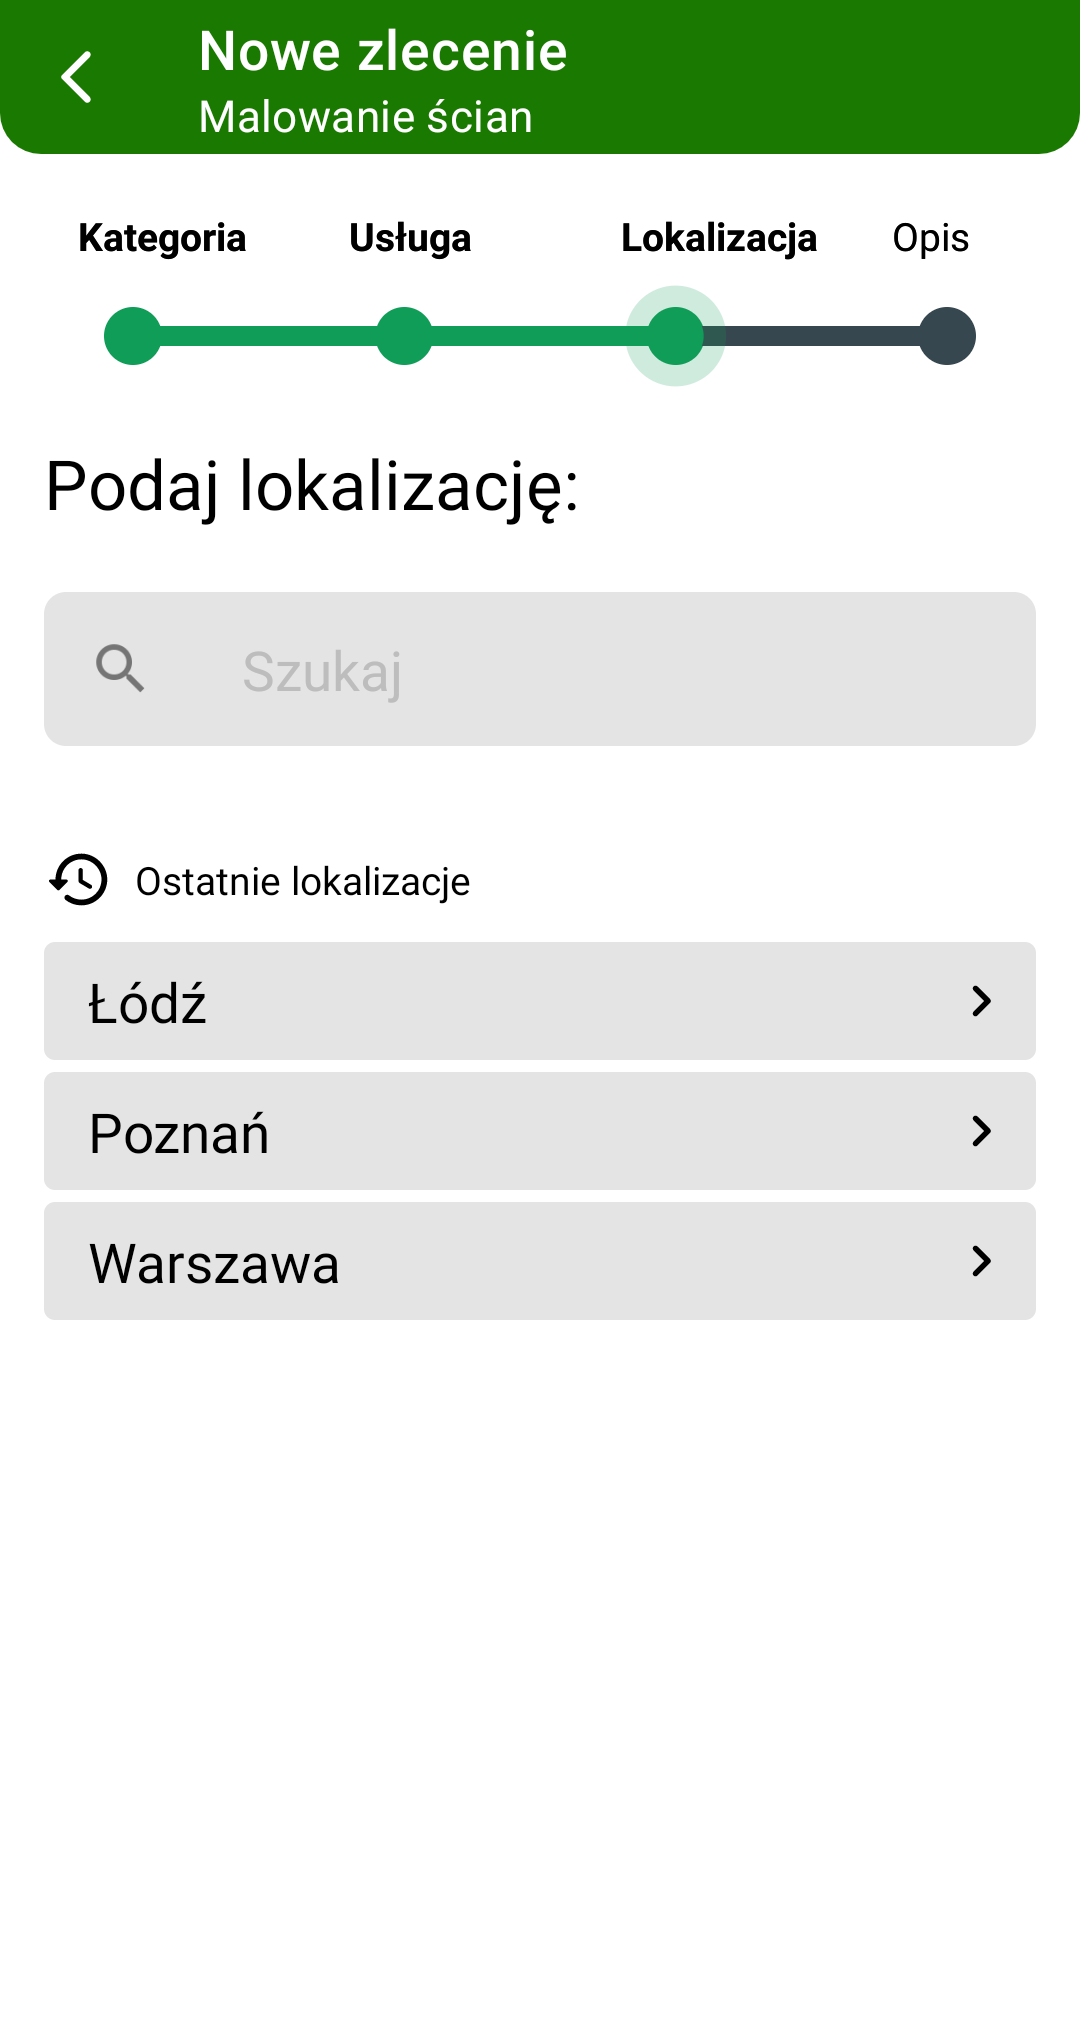
\includegraphics[width=0.97\linewidth]{screens/add_job_location.png}}
    \caption{Ekran wyboru lokalizacji}
  \end{subfigure}
  \vskip\baselineskip
  \vskip\baselineskip
  \vskip\baselineskip
  \begin{subfigure}[t]{0.32\textwidth}
    \centering
    \fbox{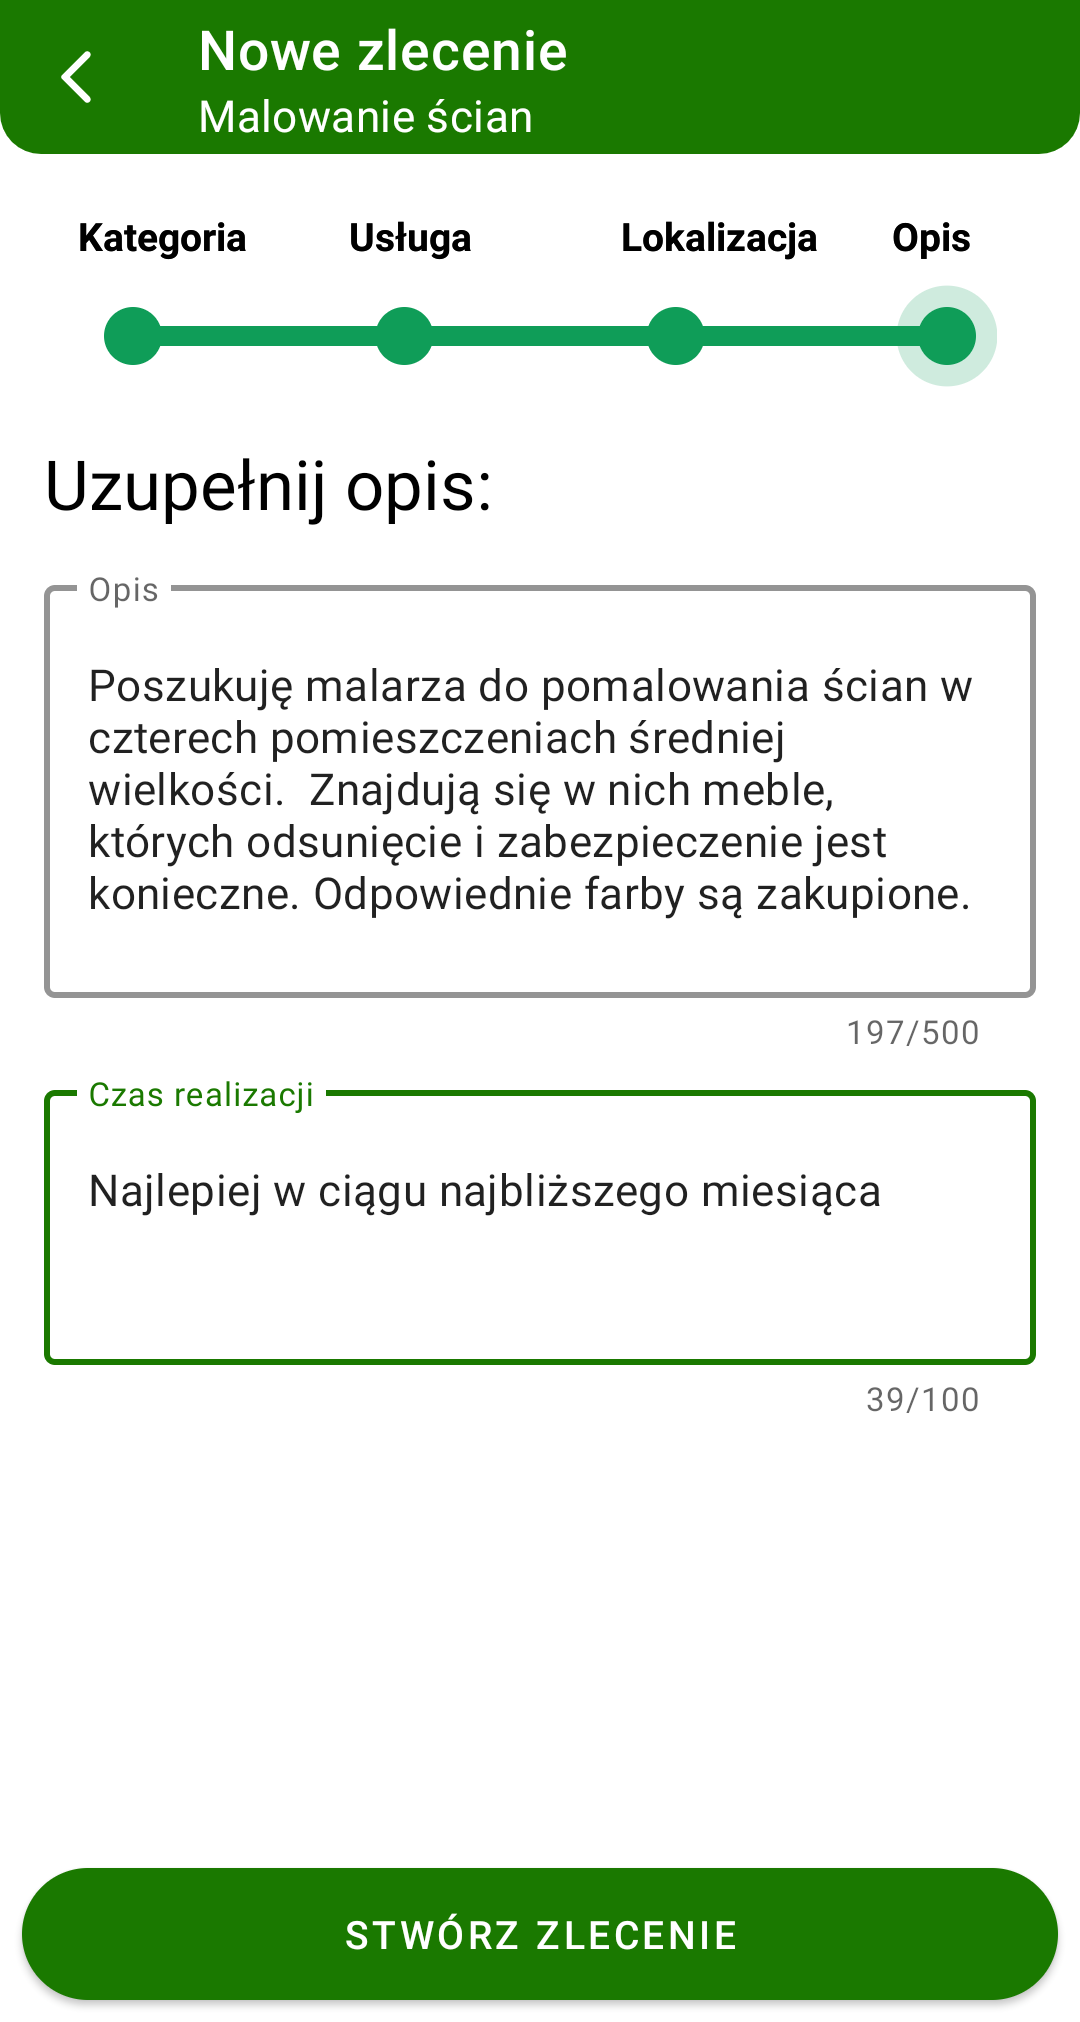
\includegraphics[width=0.97\linewidth]{screens/add_job_details.png}}
    \caption{Ekran uzupełnienia opisu}
  \end{subfigure}
  \begin{subfigure}[t]{0.32\textwidth}
    \centering
    \fbox{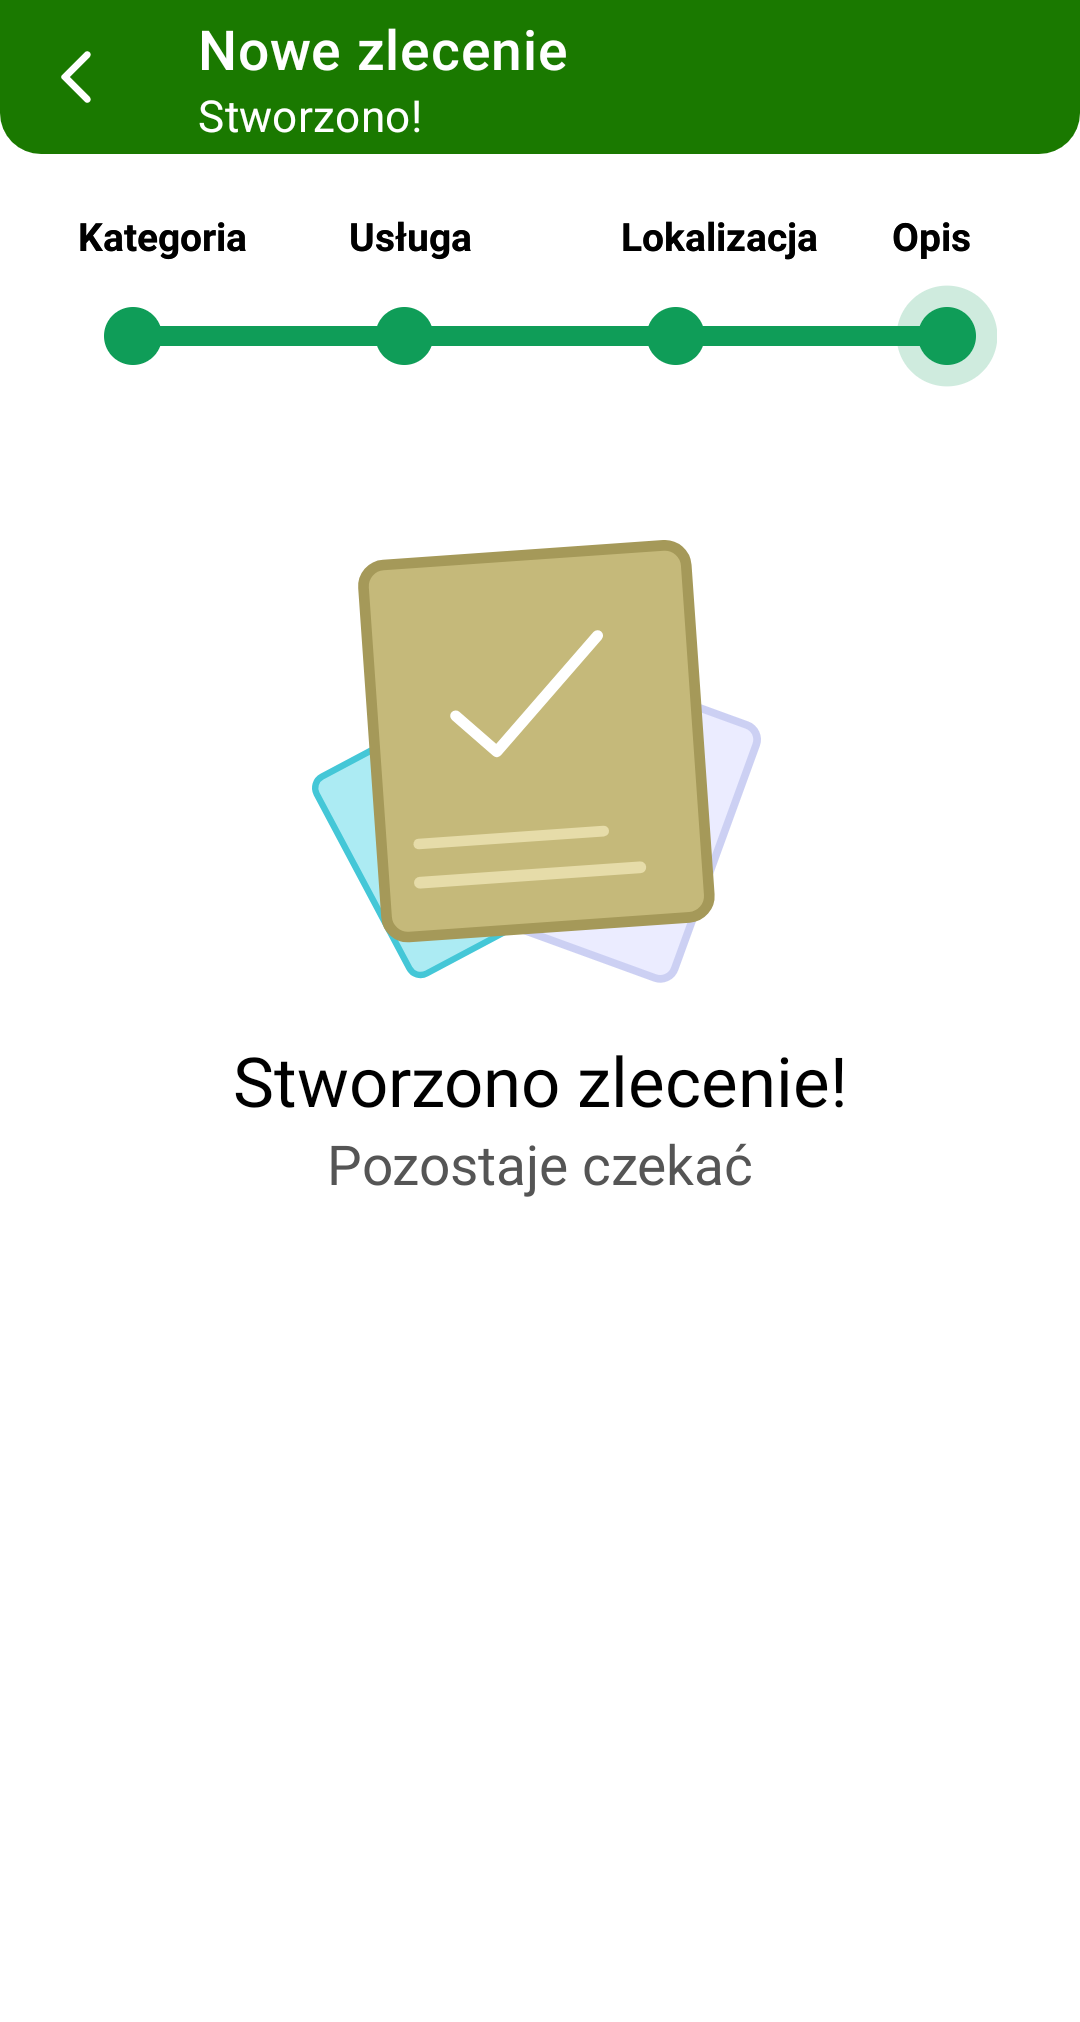
\includegraphics[width=0.97\linewidth]{screens/add_job_done.png}}
    \caption{Ekran potwierdzenia dodania}
  \end{subfigure}
  \caption{Ekrany dodawania zlecenia}
  \label{fig:add-job}
\end{figure}
\section{Akceptowanie i odrzucanie zleceń}

Utworzone przez klienta zlecenie wysyłane jest do wszystkich wykonawców, którzy świadczą żądaną usługę w pobliżu zadanej lokalizacji. Mogą je wówczas zaakceptować lub odrzucić. W tej sekcji zaprezentowane zostaną elementy, które to umożliwiają. Odpowiednie ekrany przedstawiono na rysunku \ref{fig:expert-jobs}.

\begin{figure}[ht]
  \captionsetup[subfigure]{justification=centering}
  \centering
  \begin{subfigure}[t]{0.32\textwidth}
    \centering
    \fbox{
\includegraphics[width=0.97\linewidth]{screens/expert_jobs_swap.png}}
    \caption{Widok dostępnych dla wykonawcy zleceń}
  \end{subfigure}
  \begin{subfigure}[t]{0.32\textwidth}
    \centering
    \fbox{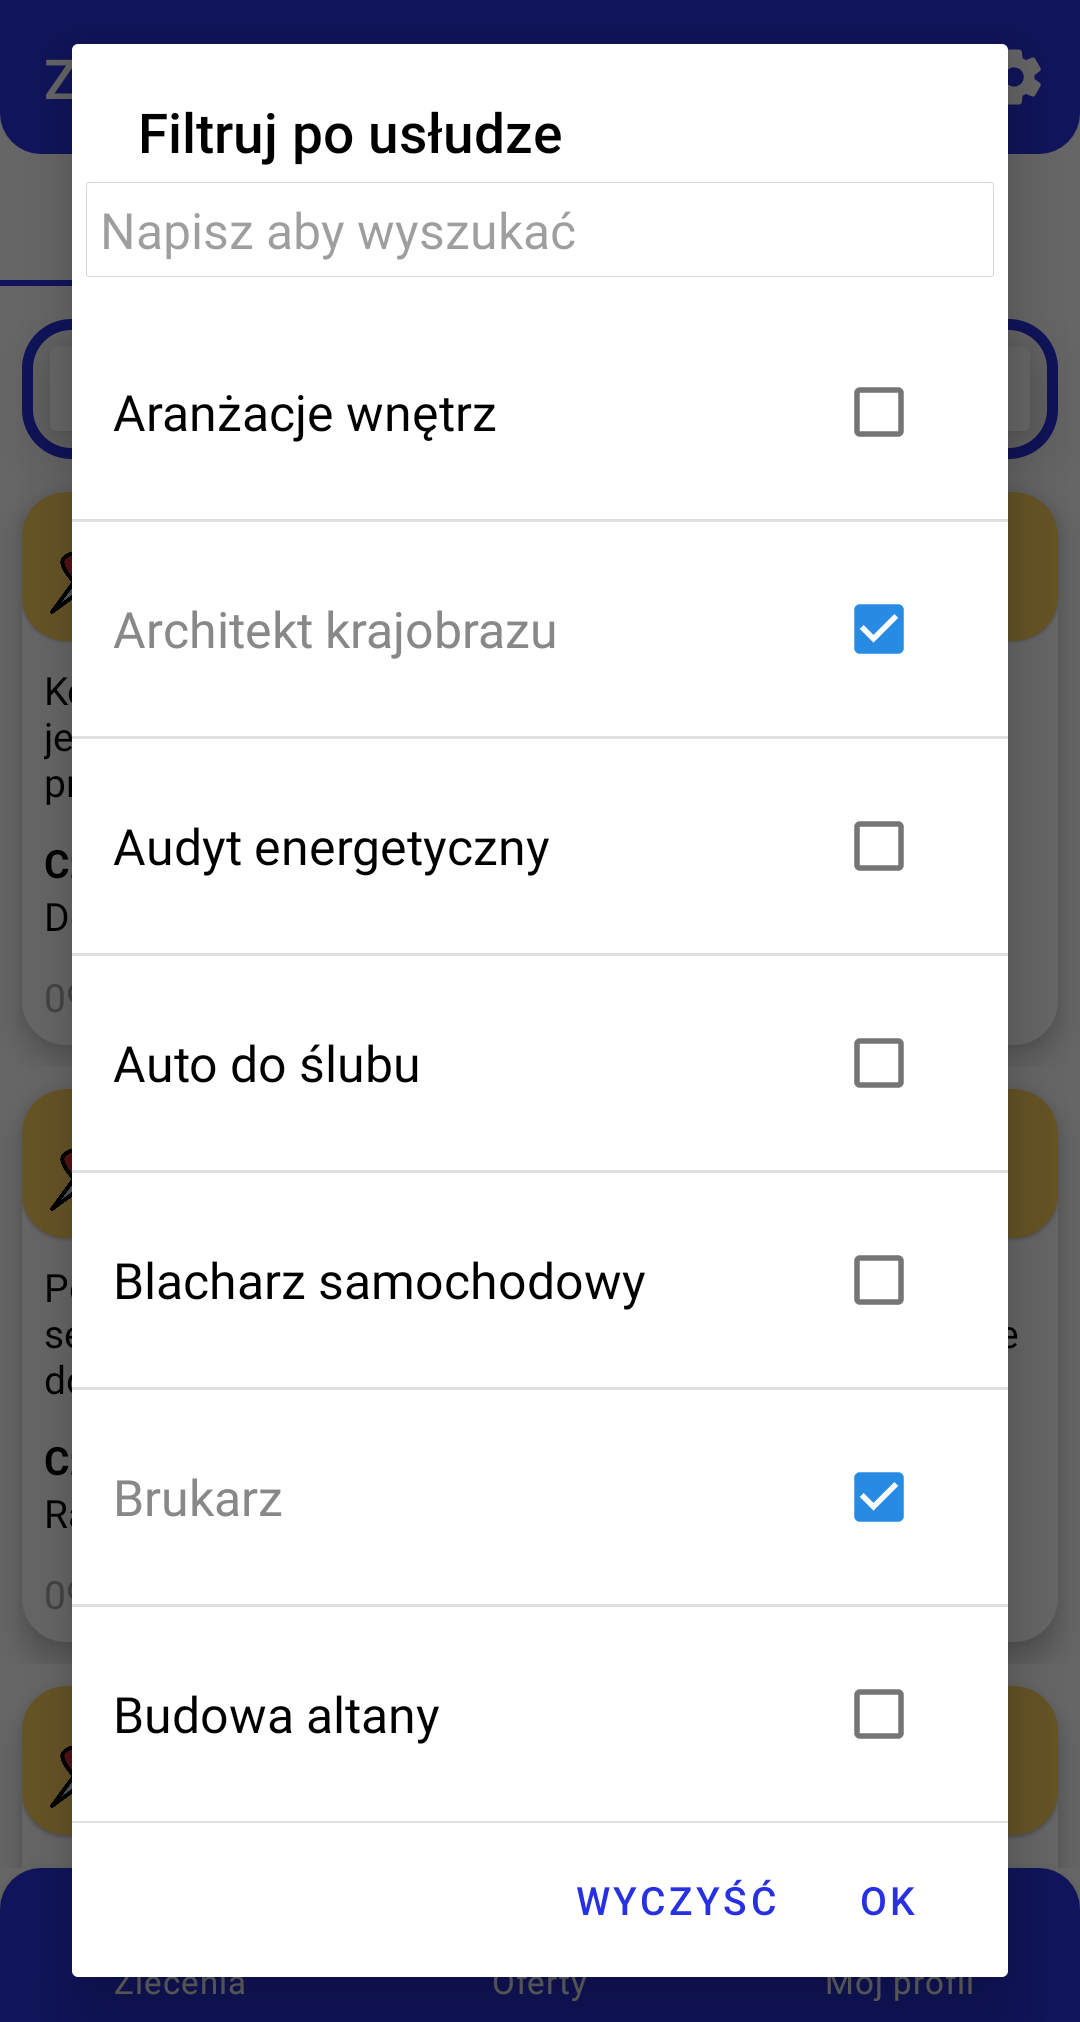
\includegraphics[width=0.97\linewidth]{screens/expert_jobs_filter.png}}
    \caption{Widok okna dialogowego filtrowania}
  \end{subfigure}
  \begin{subfigure}[t]{0.32\textwidth}
    \centering
    \fbox{
\includegraphics[width=0.97\linewidth]{screens/expert_job.png}}
    \caption{Widok szczegółów zlecenia}
  \end{subfigure}
  \caption{Ekrany umożliwiające akceptowanie i odrzucanie zleceń przez wykonawcę}
  \label{fig:expert-jobs}
\end{figure}

Dostępne dla wykonawcy zlecenia zostały podzielone na dwie kategorie: nowe oraz odrzucone. Można pomiędzy nimi przełączać się z wykorzystaniem zakładek. Dzięki temu, gdy zlecenie zostanie odrzucone, to nie znika bezpowrotnie. Zostaje jedynie przeniesione do kategorii odrzuconych, skąd wykonawca może je przyjąć wtedy, gdy jednak zmieni zdanie. Może się tak zdarzyć na przykład, gdy skończy bieżącą pracę szybciej, niż to przewidywał.

Lista zleceń może być długa, z tego powodu podczas implementacji zastosowano technikę zwaną stronicowaniem. Umożliwia ona pobieranie z bazy danych jedynie tych elementów, które w danej chwili są widoczne na ekranie. Pozwala to zmniejszyć transfer informacji i koszty generowane przez Firebase. 

Aby ułatwić wykonawcom przeszukiwanie zleceń dodano funkcję filtrowania za pomocą nazw usług. Odpowiedzialny za to komponent znajduje się na szczycie listy i jego kliknięcie otwiera okno dialogowe. Są w nim umieszczone wszystkie świadczone usługi i można dokonać ich wielokrotnego wyboru.

Wybranie konkretnego zlecenia z listy przenosi użytkownika do ekranu szczegółów. Jeżeli jest ono nowe, to ekran zawiera przyciski do akceptacji i odrzucenia. Jeżeli natomiast jest już odrzucone, to widoczny jest jedynie pierwszy przycisk. Kliknięcie go powoduje przyjęcie zlecenia i usunięcie z listy dostępnych. 

Przewidziana została również funkcja szybkiego odrzucenia zlecenia. Polega ona na prostym przeciągnięciu wybranego elementu na liście w prawo. Stwierdzono bowiem, że już widoczne tam informacje mogą skłonić do tego wykonawcę i nie trzeba go zmuszać do otwierania ekranu szczegółów.

Poza filtrowaniem zleceń po nazwach usług przydatne mogłoby być również przeszukiwanie ich po nazwiskach klientów, czy też opisie. Taka funkcjonalność nie wydaje się powierzchownie trudna w implementacji, lecz baza Firebase Firestore nie umożliwia przeszukiwania pełnotekstowego. Aby je zapewnić konieczne byłoby wsparcie się dodatkową, zewnętrzną usługą przeszukiwania, na przykład Elasticsearch \cite{elasticsearch}. Rozważano taką możliwość, lecz uznano, że ta funkcja nie jest krytyczna, a stosunkowo duży wysiłek, potrzebny do jej zaimplementowania, lepiej przeznaczyć na inne części systemu.
\section{Przeglądanie zleceń przez klientów}

Klienci muszą posiadać możliwość przeglądania utworzonych przez siebie zleceń. Ekran, który taką funkcjonalność zapewnia, został przedstawiony na rysunku \ref{fig:client-jobs}. Zawiera on listę zleceń, którą można ograniczyć do konkretnych usług przy pomocy mechanizmu filtrowania.
%  Lista jest posortowana chronologicznie, najnowsze zlecenia znajdują się na jej szczycie.
Elementy listy zawierają ikonkę pinezki, której kolor zdradza, czy dane zlecenie jest jeszcze otwarte i czy wykonawcy mogą się dalej zgłaszać. Jeśli tak jest, to ma ona kolor zielony, a w przeciwnym wypadku kolor czerwony. Jeżeli miały miejsce jakieś zdarzenia dotyczące zlecenia, które nie zostały jeszcze odczytane, to wewnątrz elementu listy wyświetlana jest taka informacja. 
%Wybranie z listy któregoś ze zleceń spowoduje przejście do ekranu zgłoszonych ofert. Opisano go w kolejnej sekcji.

\begin{figure}[ht!]
  \centering
    \fbox{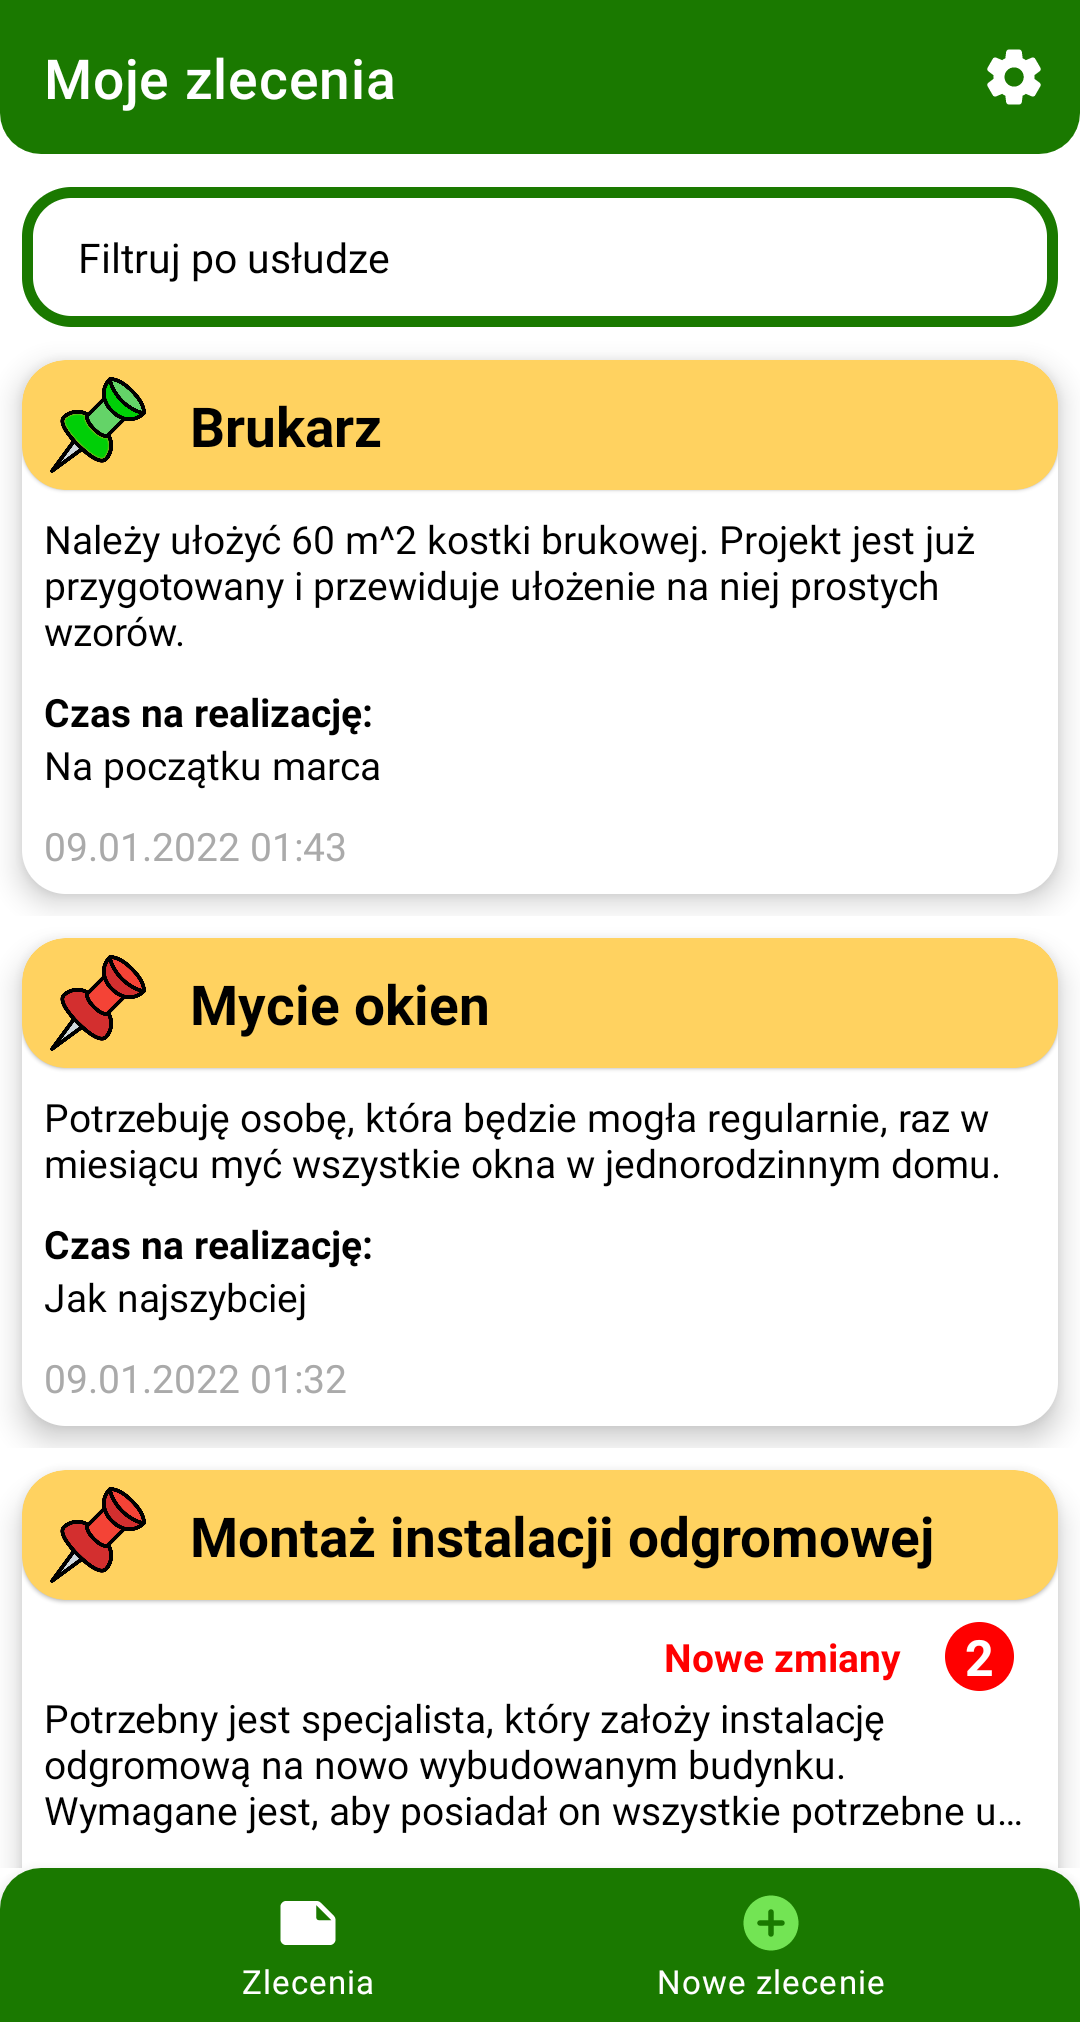
\includegraphics[width=0.33\linewidth]{screens/client_jobs.png}}
  \caption{Ekran listy utworzonych przez klienta zleceń}
  \label{fig:client-jobs}
\end{figure}

\section{Przeglądanie ofert}

Zarówno klienci, jak i wykonawcy posiadają możliwość przeglądania ofert, lecz w nieco innym kontekście. Pierwsi mogą zobaczyć te, które zostały złożone do utworzonych przez siebie zleceń, a drudzy te, które sami złożyli.

W celu jasnego wyrażenia stanu ofert postanowiono wprowadzić dla nich  cztery  możliwe statusy: nowe, anulowane, w realizacji, wykonano. Stanowią one sposób na etykietowanie ofert oraz zapewniają spójny sposób ich postrzegania przez obie strony. Zostały one stworzone z myślą o wykorzystaniu w następujący sposób:

\begin{itemize}
    \item nowe - jedynie dla nowo utworzonych ofert;
    \item anulowane - gdy współpraca została porzucona;
    \item w realizacji - gdy współpraca została potwierdzona;
    \item wykonano - gdy usługa została wykonana.
\end{itemize}

% Założono, że każda oferta będzie posiadała status, na będzie jasno wyrażał etap na którym znajdują się prace. Założono istnienie następujących statusów: nowe, anulowane, w realizacji, wykonano. Status nowej oferty jest przyznawany nowo stworzonym, którym nie zdążono przypisać jeszcze innego. Jeżeli klient lub wykonawca postanowi zrezygnować ze współpracy, to może zmienić status na \enquote{anulowane}, a w przeciwnym wypadku na \enquote{w realizacji}. W chwili, gdy usługa zostanie wykonana to status powinien zostać zmieniony przez jednego z nich na \enquote{wykonane}. Takie podejście znacznie ułatwia pracę z duża liczbą ofert i umożliwia filtrowanie po statusie, które zastosowano.

Na rysunku \ref{fig:offers-client} zamieszczono ekran ofert, które zostały zgłoszone do utworzonego przez klienta zlecenia. Są przedstawione w postaci listy, której każdy element zawiera podstawowe informacje o wykonawcy, ostatnią wiadomość z chatu oraz status. Jeśli istnieją nieodczytane wiadomości lub oferta jest nowa, to zostaje ona wyróżniona. Dostępna jest możliwość filtrowania opisywanej listy przy pomocy statusów ofert. Klient, jako twórca zlecenia, ma również możliwość zobaczenia planowanej daty jego zamknięcia oraz wykonania tego wcześniej.

\begin{figure}[ht!]
  \captionsetup[subfigure]{justification=centering}
  \centering
  \begin{subfigure}[t]{0.32\textwidth}
    \centering
    \fbox{
\includegraphics[width=0.97\linewidth]{screens/client_offers_open.png}}
    \caption{Widok otwartego zlecenia}
  \end{subfigure}
  \begin{subfigure}[t]{0.32\textwidth}
    \centering
    \fbox{
\includegraphics[width=0.97\linewidth]{screens/client_offers_closed.png}}
    \caption{Widok zamkniętego zlecenia}
  \end{subfigure}
  \caption{Ekran listy ofert zgłoszonych do zlecenia}
  \label{fig:offers-client}
\end{figure}

Dla wykonawców ekran ofert został przedstawiony na rysunku \ref{fig:offers-expert}. Zastosowano w nim dodatkowo podział na dwie kategorie: aktualne oraz archiwalne. Uznano to za przydatne, ponieważ spodziewano się, że wykonawcy będą pracować ze znacznie większą liczbą ofert niż klienci. Dzięki zastosowanemu podziałowi mogą przechowywać jako aktualne tylko te, które w danym momencie mają dla nich znaczenie. Przeniesienia pomiędzy kategoriami dokonuje się poprzez przeciągnięcie wybranej oferty w prawo. 

% Z powodu wspomnianej, możliwie dużej liczby ofert, w aplikacji dla wykonawców zastosowano stronicowanie. Dla aplikacji dla klientów nie było to konieczne, ponieważ liczebność ofert na liście nie mogła przekroczyć tam maksymalnej liczby ośmiu.

% Oprócz samych ofert na ekranie klienta została umieszczona ich aktualna i maksymalna liczba oraz data zakończenia zlecenia. Informacja ta znajduję się w widocznym miejscu, ponieważ po zapełnieniu liczby ofert lub minięciu terminu kolejni wykonawcy nie będą mogli się zgłaszać. Odpowiedni przycisk umożliwia również wcześniejsze zakończenie zlecenia, na przykład jeśli wykonawca do realizacji usługi zostanie już wybrany.

\begin{figure}[ht!]
  \captionsetup[subfigure]{justification=centering}
  \centering
  \begin{subfigure}[t]{0.32\textwidth}
    \centering
    \fbox{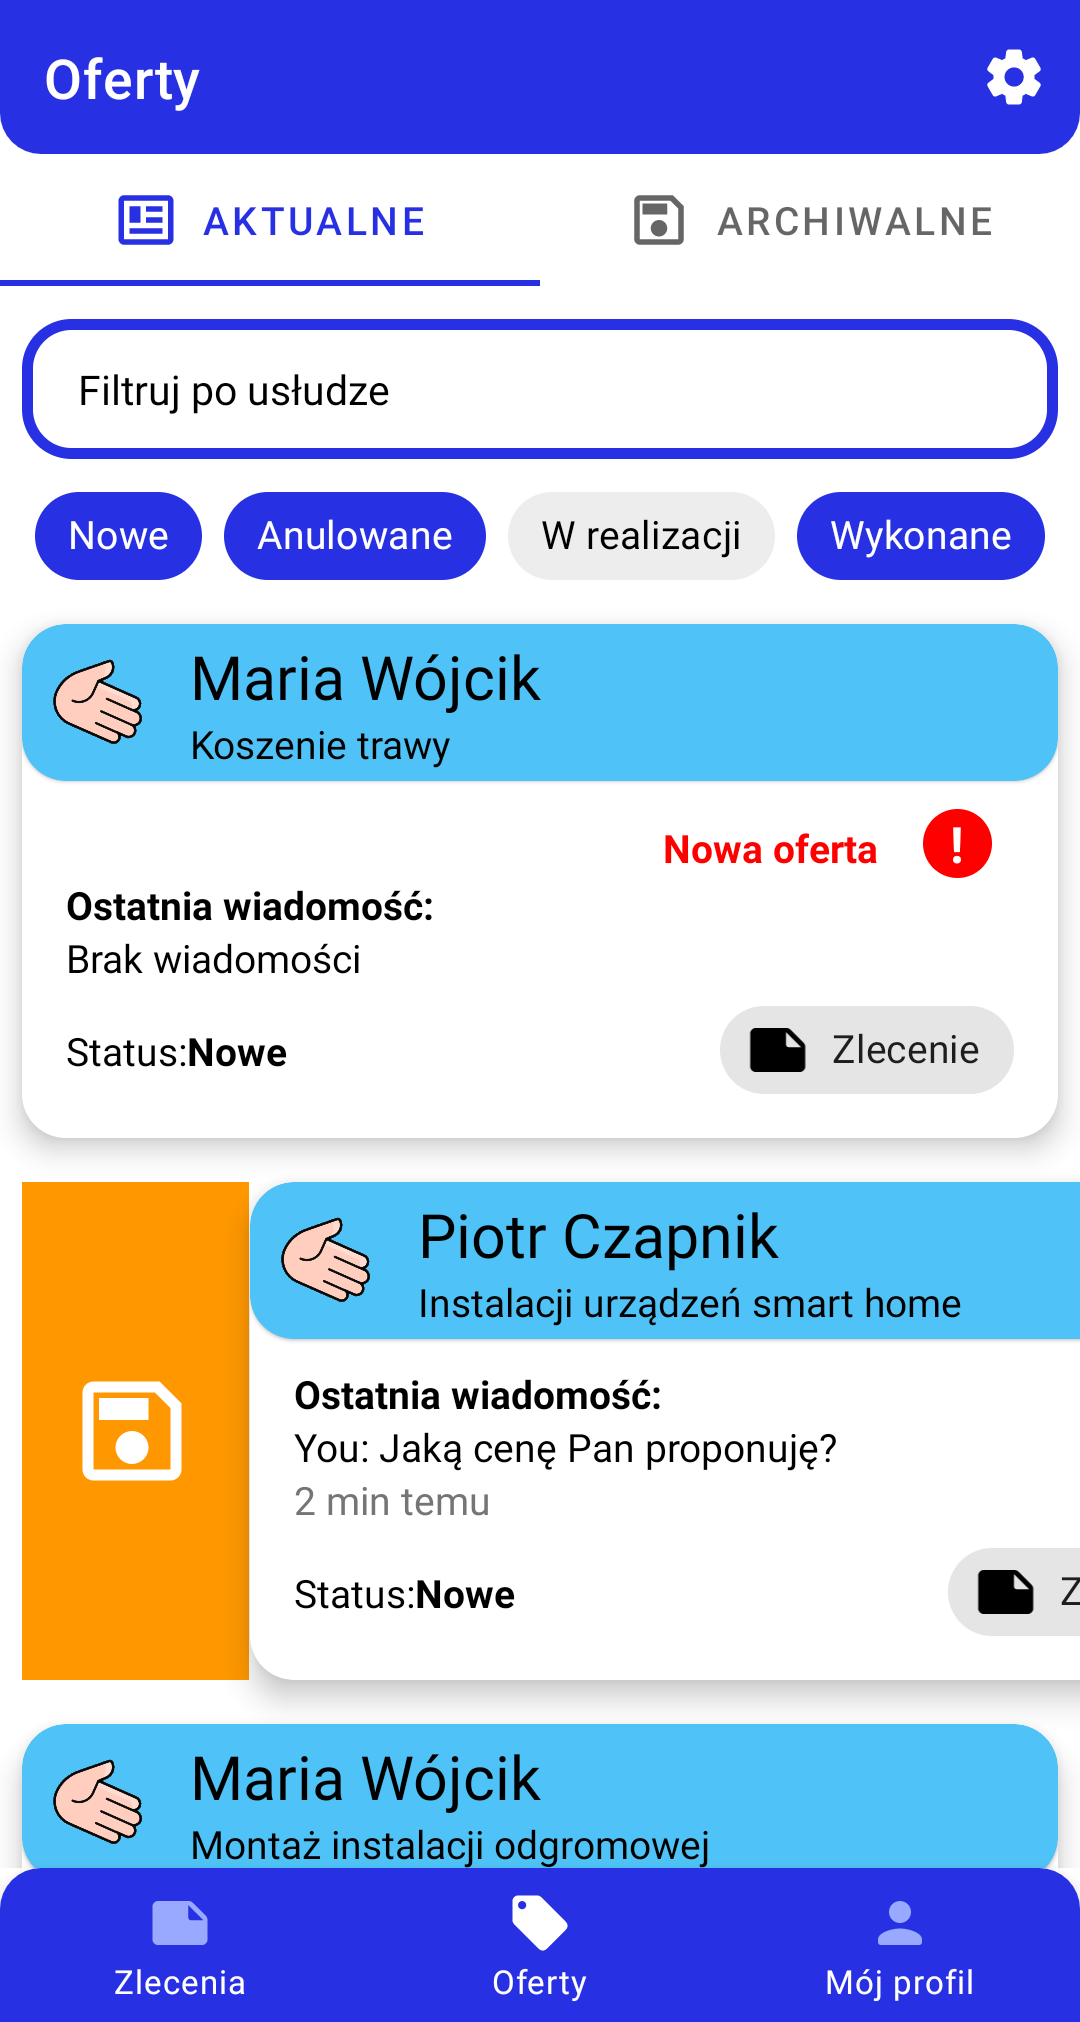
\includegraphics[width=0.97\linewidth]{screens/expert_offers_current.png}}
    \caption{Widok aktualnych ofert}
  \end{subfigure}
  \begin{subfigure}[t]{0.32\textwidth}
    \centering
    \fbox{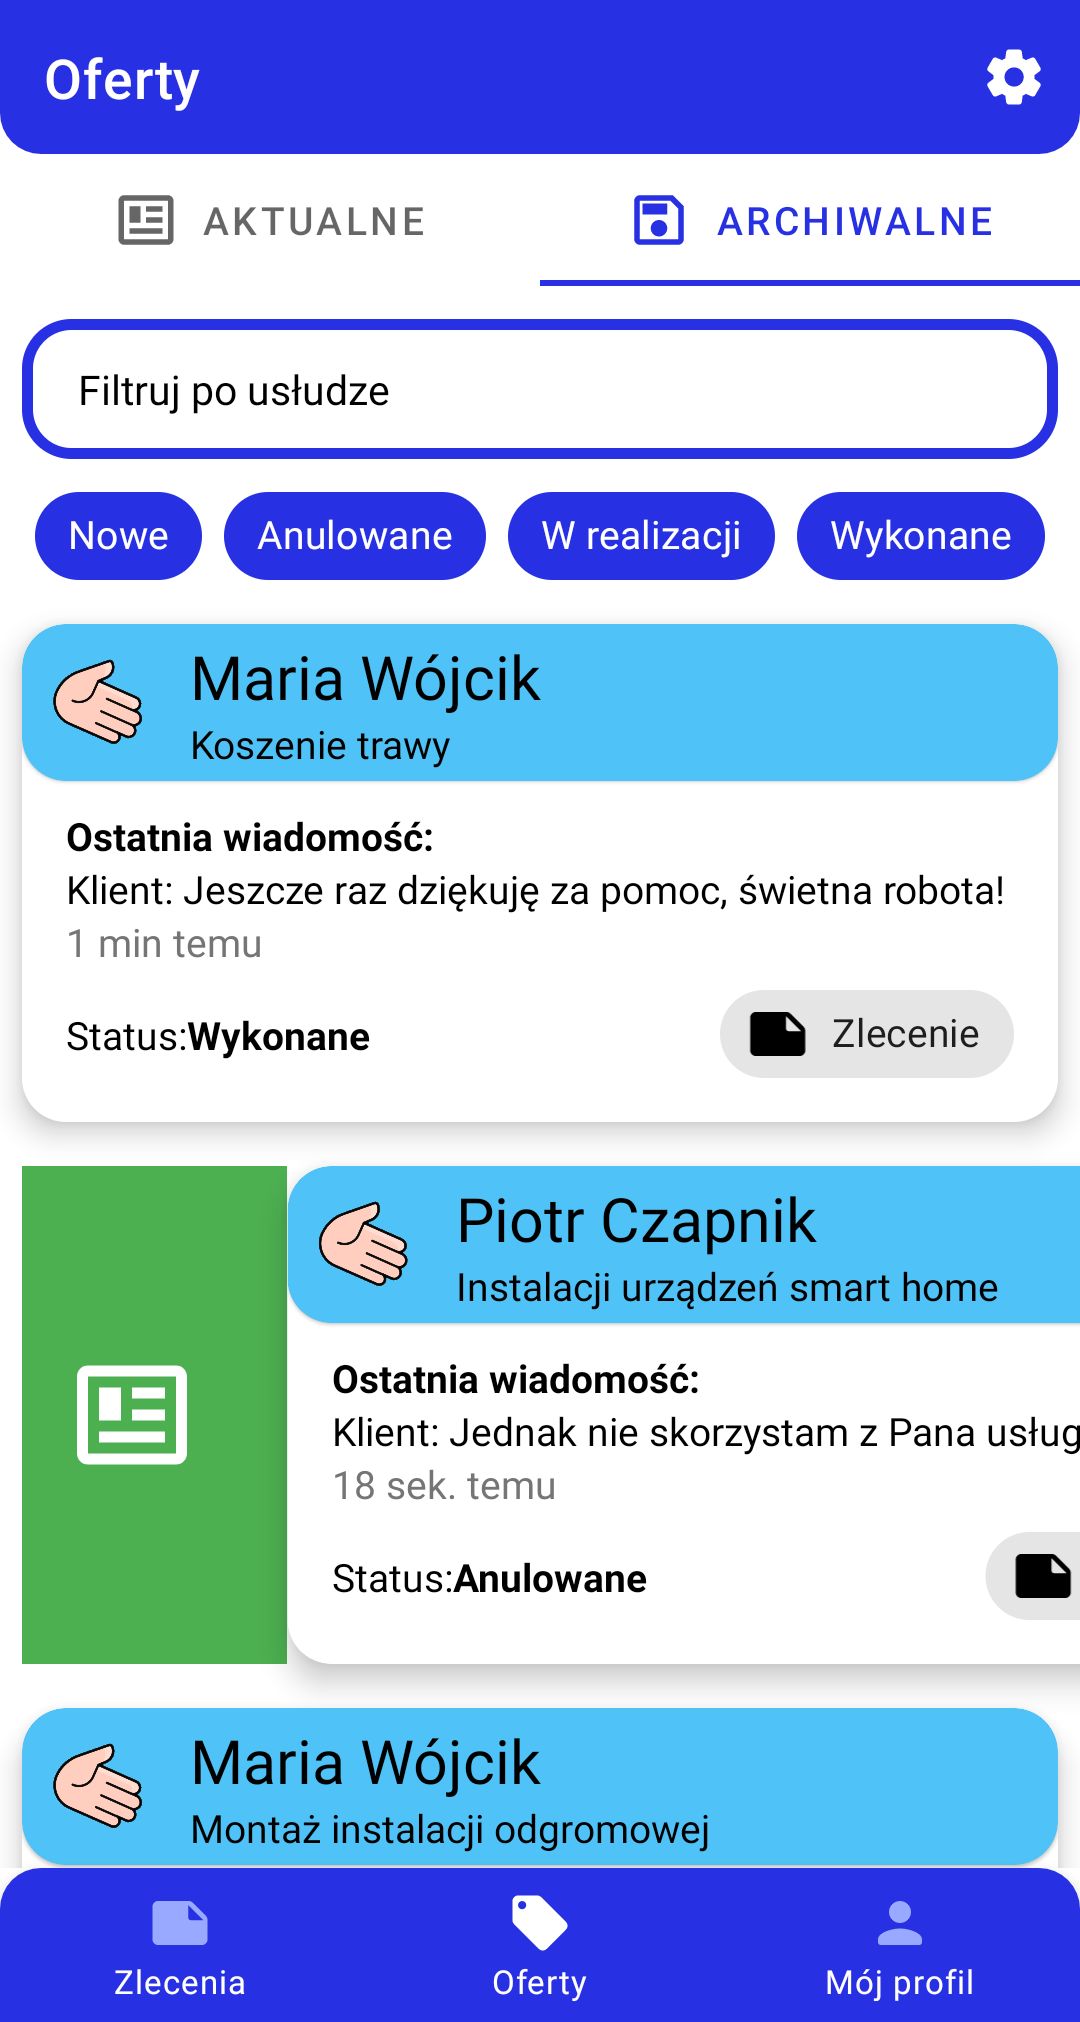
\includegraphics[width=0.97\linewidth]{screens/expert_offers_archived.png}}
    \caption{Widok archiwalnych ofert}
  \end{subfigure}
  \caption{Ekran listy złożonych przez wykonawcę ofert}
  \label{fig:offers-expert}
\end{figure}


\section{Chat}

Chat to bardzo ważna funkcjonalność, która zapewnia istnienie podstawowego kanału komunikacyjnego pomiędzy klientem i wykonawcą. Ekran chatu, z uwzględnieniem obu aplikacji, przedstawiono na rysunku \ref{fig:chat}. Składa się on z kilku części: paska aplikacji, paska statusu oferty, panelu odebranych wiadomości oraz wysyłania nowych.

Na pasku aplikacji umieszczona jest ikona umożliwiająca połączenie telefoniczne z drugą stroną. Jest ono jednak dostępne jedynie wtedy, kiedy uzupełniła ona swój numer telefonu. Jest on bowiem zarówno dla klientów, jak i wykonawców opcjonalny. Na tym pasku jest również umieszczona ikona umożliwiająca rozwinięcie innych opcji. Znajdują się tam elementy zależne od aplikacji. Klienci mają możliwość zobaczenia profilu wykonawcy oraz dodania lub zobaczenia oceny. Wykonawcy mogą natomiast zobaczyć szczegóły zlecenia, przenieść je do archiwalnych lub w drugą stronę oraz zobaczyć ocenę, jeśli jest dodana.

Pasek statusu oferty informuje o aktualnym statusie oraz umożliwia jego zmianę. Po wybraniu innego niż aktualny wyświetlone zostanie okno dialogowe z prośbą o potwierdzenie. Po wykonaniu tej czynności jej status się zmienia, a na chacie zostaje wysłana wiadomość o tym mówiąca.

\begin{figure}[ht]
  \captionsetup[subfigure]{justification=centering}
  \centering
  \begin{subfigure}[t]{0.32\textwidth}
    \centering
    \fbox{
\includegraphics[width=0.97\linewidth]{screens/chat_client.png}}
    \caption{Widok aplikacji dla klientów}
  \end{subfigure}
  \begin{subfigure}[t]{0.32\textwidth}
    \centering
    \fbox{
\includegraphics[width=0.97\linewidth]{screens/chat_expert.png}}
    \caption{Widok aplikacji dla wykonawców}
  \end{subfigure}
  \caption{Ekran chatu}
  \label{fig:chat}
\end{figure}

Panel wiadomości zawiera po prawej stronie wiadomości wysyłane, a po lewej odbierane. Występują ich cztery rodzaje: tekstowe, zdjęcia, informujące o zmianach statusu oraz dodaniu komentarza. Są przechowywane w bazie danych we wspólnej kolekcji, lecz dokumenty je reprezentujące posiadają różny zestaw pól, w zależności od wspomnianego typu wiadomości.
Gdy konwersacja zostanie przesunięta do góry, to na dole pojawia się ikona strzałki, która umożliwia szybki powrót do wiadomości najnowszych. Wśród wiadomości widoczna jest również pozioma linia, która jasno oddziela wiadomości odczytane przez rozmówcę od tych nieodczytanych.

Ostatnim elementem jest panel wysyłania wiadomości. Umożliwia on przesyłanie zdjęć oraz komunikatów tekstowych. Dla tych ostatnich operacja jest możliwa do wykonania offline. Obok takich wiadomości wyświetli się informacja o aktualnym braku możliwości wysłania i zostanie to dokonane zaraz po przywróceniu połączenia z siecią. Jest to możliwe dzięki wbudowanemu w bazę Firebase Firestore mechanizmowi pracy offline. Magazyn plików Firebase Storage podobnej funkcjonalności nie posiada i w przypadku braku internetu wysyłanie zdjęcia zwyczajnie się nie powiedzie. Zostanie za to wyświetlony przyjazny komunikat z możliwością ponowienia operacji.
\section{Profil wykonawcy i komentarze}

Dla klientów bardzo ważna jest możliwość przeglądania informacji dotyczących wykonawców. Na ich podstawie mogą bowiem opierać podejmowane przez siebie decyzje. Wykonawcy również potrzebują podobnej możliwości, by móc zobaczyć informacje dotyczące siebie samych. Z tych powodów funkcjonalność przeglądania profilu wykonawcy i komentarzy została dodana do obu aplikacji.

\begin{figure}[ht]
  \captionsetup[subfigure]{justification=centering}
  \centering
  \begin{subfigure}[t]{0.32\textwidth}
    \centering
    \fbox{\includegraphics[width=0.97\linewidth]{screens/profile_1.png}}
  \end{subfigure}
  \begin{subfigure}[t]{0.32\textwidth}
    \centering
    \fbox{\includegraphics[width=0.97\linewidth]{screens/profile_2.png}}
  \end{subfigure}
  \begin{subfigure}[t]{0.32\textwidth}
    \centering
    \fbox{\includegraphics[width=0.97\linewidth]{screens/profile_3.png}}
  \end{subfigure}
  \caption[Ekran profilu wykonawcy]{Ekran profilu wykonawcy w aplikacji dla klientów}
  \label{fig:profile}
\end{figure}

Okazuje się, że przeprowadzone zostały dokładne badania dotyczące strategii podejmowania decyzji przez klientów podczas zakupów online. W jednym z artykułów \cite{ratings-presentation} stwierdza się, że pomimo tego, iż mają oni zwykle dostępnych wiele źródeł informacji, to często szukają możliwości uproszczenia swoich decyzji i wyciągnięcia sedna. Z tego powodu postanowiono umieścić w widocznym miejscu średnią ocenę wykonawcy, która jest dobrym wskaźnikiem do tego celu. Można to zobaczyć na rysunku \ref{fig:profile}.

Na ekranie profilu wykonawcy postanowiono umieścić jedynie trzy ostatnio dodane komentarze. W celu zobaczenia pełnej listy konieczne jest przejście do oddzielnego ekranu, na którym się one znajdują. Ponieważ niektóre mogą być długie, postanowiono je przyciąć do długości trzech linii. Aby zobaczyć wówczas całą treść należy wybrać konkretny komentarz. Odpowiednie widoki przedstawiono na rysunku \ref{fig:ratings}.

\begin{figure}[ht]
  \captionsetup[subfigure]{justification=centering}
  \centering
  \begin{subfigure}[t]{0.32\textwidth}
    \centering
    \fbox{\includegraphics[width=0.97\linewidth]{screens/ratings.png}}
    \caption{Ekran wszystkich komentarzy}
  \end{subfigure}
  \begin{subfigure}[t]{0.32\textwidth}
    \centering
    \fbox{\includegraphics[width=0.97\linewidth]{screens/rating.png}}
    \caption{Ekran wybranego komentarza}
  \end{subfigure}
  \caption{Ekrany komentarzy}
  \label{fig:ratings}
\end{figure}

\section{Ocenianie wykonawców}

Ocenianie wykonawców to dość prosta funkcjonalność, którą posiadają klienci. Składa się na nią jeden ekran przedstawiony na rysunku \ref{fig:rate}. Ocena dokonywana jest poprzez zaznaczenie odpowiedniej liczby gwiazdek oraz wpisane opcjonalnego komentarza. Można dokonać jej tylko raz dla każdej oferty, bez możliwości późniejszej edycji.

Szczególnie zastanawiano się nad wyborem odpowiedniej metody, za pomocą której klienci mają wyrażać poziom swojej satysfakcji. Pomocny przy tym zagadnieniu okazał się artykuł Roberta Westbrooka \cite{rating-scale}, który porównuje efektywność mierzenia satysfakcji za pomocą różnych skal. Szczególnie zachęca do wykorzystania skali DT (ang. Delighted - Terrible), która wprowadza bardziej równomierny rozkład dla oddawanych ocen niż inne. Zdecydowano się jednak wykorzystać gotowy już komponent paska gwiazdek, by uniknąć problemów z implementacją. Z tego powodu dodano jedynie wyświetlany nad nim napis odpowiadający aktualnej jego wartości w skali DT, na przykład: neutralnie, raczej satysfakcjonująco, zadowalająco, czy zachwycająco. Poprzez taki zabieg miano nadzieję wykorzystać część korzyści płynących ze skali DT, bez nadmiernego nakładu pracy. Nie jest to bowiem element kluczowy.

\begin{figure}[ht]
  \centering
    \fbox{\includegraphics[width=0.33\linewidth]{screens/add_rating.png}}
  \caption{Ekran oceniania wykonawcy}
  \label{fig:rate}
\end{figure}

Wadą stworzonego systemu ocen, którą należy wskazać i zaznaczyć, jest to, że nie jest on do końca wiarygodny. Problem polega na tym, iż nieuczciwi wykonawcy mogą się zarejestrować również jako klienci, a następnie podjąć działania, których wynikiem będzie wystawienie samemu sobie pozytywnej oceny. Problem ten okazał się bardzo trudnym do rozwiązania. Najprostszym wyjściem jest zablokowanie możliwości oceniania, gdy konwersacja jest pusta lub zlecenie zostało dopiero utworzone. Są to jasne przesłanki co do próby oszustwa, lecz takie zabezpieczenie jest proste do obejścia. Bardziej rzetelną metodą byłaby konieczność walidacji wszystkich komentarzy przez moderatorów, którzy mieliby dostęp do konwersacji i pozostałych informacji. Mimo wszystko wciąż nie jest to rozwiązanie pewne, ponieważ informacje te mogły zostać w dobry sposób spreparowane. Z technicznego punktu widzenia dla moderatorów potrzebny byłby również kolejny interfejs, co wiążę się z dalszą komplikacją projektu. Z wymienionych przyczyn postanowiono zaakceptować brak pełnej wiarygodności ocen i zostawić rozwiązanie tego problemu na ewentualne dalsze etapy rozwoju projektu.
\section{Usuwanie konta}

Usuwanie kont klienta oraz wykonawcy okazało się bardziej skomplikowanym w implementacji, niż się tego spodziewano. Wymagało ono przeprowadzenia licznych operacji w bazie danych oraz dodatkowych założeń. Przyjęto, że usunięcie konta klienta pozostawi wszystkie dodane przez niego oceny i komentarze nienaruszone, aby inni mogli wciąż na nich bazować. Znikną one dopiero wraz z usunięciem wykonawcy. Pozostawiane są również wszystkie oferty klienta, ponieważ wykonawcy wciąż mogą mieć do nich dostęp. Są one usuwane dopiero, gdy obie strony go stracą. Z kolei zlecenia są usuwanie wtedy, gdy zarówno klient będący ich twórcą, jak i wszystkie zgłoszone oferty zostaną usunięte. W implementacji tych zależności pomogły funkcje wywoływane modyfikacją danych, dostępne w ramach Firebase Functions. 

\begin{figure}[ht]
  \captionsetup[subfigure]{justification=centering}
  \centering
  \begin{subfigure}[t]{0.32\textwidth}
    \centering
    \fbox{\includegraphics[width=0.97\linewidth]{screens/delete.png}}
    \caption{Ekran usuwania konta klienta}
  \end{subfigure}
  \begin{subfigure}[t]{0.32\textwidth}
    \centering
    \fbox{\includegraphics[width=0.97\linewidth]{screens/delete_offers.png}}
    \caption{Widok usuniętego klienta na liście ofert}
  \end{subfigure}
  \begin{subfigure}[t]{0.32\textwidth}
    \centering
    \fbox{\includegraphics[width=0.97\linewidth]{screens/delete_offer.png}}
    \caption{Ekran chatu z usuniętym klientem}
  \end{subfigure}
  \caption{Ekrany związane z usuwaniem konta}
  \label{fig:delete}
\end{figure}

Na rysunku \ref{fig:delete} przedstawiono ekrany związane z usuwaniem konta przez klienta. Aby operacja mogła zostać wykonana użytkownik musi wpisać w polu tekstowym słowo \enquote{Potwierdzam}. Jest to zabezpieczenie przeciwko przypadkowemu i niechcianemu działaniu. Gdy konto zostanie usunięte, to użytkownicy, którzy wchodzili z nim wcześniej w interakcję zobaczą o tym powiadomienie przy odpowiedniej ofercie. Nie będą mieli od tej pory możliwości komunikacji z nim za pomocą chatu, chociaż przeglądanie historii wiadomości wciąż będzie dostępne.
\section{Powiadomienia push}

Powiadomienia w systemie Android są wiadomościami wyświetlanymi poza interfejsem aplikacji, które mogą stanowić przypomnienia, komunikaty lub zachęty do wykonania pewnych czynności. Powiadomienia push są szczególnym ich rodzajem, który jest wywoływany i przesyłany przez zewnętrzny serwer. 

W stworzonym rozwiązaniu powiadomienia push zostały wykorzystane w celu informowania użytkowników o ważnych zdarzeniach, gdy nie korzystają oni akurat z aplikacji. Za ich pomocą są powiadamiani o wysłaniu wiadomości na chacie, zmianie statusu oferty, czy też dodaniu oceny. Przykładowe powiadomienie zostało przedstawione na rysunku \ref{fig:notification}.

% Ich kliknięcie powoduje uruchomienie ekranu aplikacji związanego z danym zdarzeniem.

\begin{figure}[ht!]
  \centering
    \fbox{\includegraphics[width=0.66\linewidth]{screens/notification.png}}
  \caption[Przykład powiadomienia]{Przykład powiadomienia o dodanej ocenie}
  \label{fig:notification}
\end{figure}

Powiadomienia są wykorzystywane przez wiele aplikacji, co może prowadzić do natłoku informacji oraz rozdrażnienia użytkowników. Zwrócił na to uwagę Tilo Westermann w swojej książce \enquote{User Acceptance of Mobile Notifications} \cite{notifications-acceptance}. Z jego badań wynika, że powiadomienia związane z prawdziwymi ludźmi są najmniej drażniące. Te wykorzystywane przez tworzone aplikacje można do takich zaliczyć, ponieważ są wywoływane działaniami podejmowanymi przez użytkowników. W książce zostało również stwierdzone, że aplikacje do komunikacji mogą wysyłać powiadomienia w czasie rzeczywistym, podczas gdy dla innych rodzajów warto zastanowić się nad wprowadzeniem opóźnienia, by nie przeszkadzać niepotrzebnie użytkownikom. Tworzone programy uznano za taki rodzaj aplikacji i postanowiono dostarczać powiadomienia jak najszybciej, by użytkownik był na bieżąco.

W celu stworzenia wygodnego systemu powiadomień należy wziąć pod uwagę sposób, w jaki użytkownicy je obsługują. Kwestia ta została poruszona w pewnym artykule \cite{notifications-dismissed}, w którym dokonano rozważań z zachowaniem podziału na kilka kategorii powiadomień. Okazuje się, że te wysyłane przez komunikatory są zwykle bardzo szybko obsługiwane. Z tego powodu ważne było zapewnienie możliwość wygodnego przejścia do ekranu chatu poprzez kliknięcie takiego powiadomienia.
% Brak przecinka przed poprzez

Implementację znacznie ułatwiła usługa Firebase Cloud Messaging. Z jej pomocą powiadomienia są wysyłane do odpowiednich urządzeń, identyfikowanych przy pomocy tokenów. Gdy użytkownik loguje się na nowym urządzeniu, to do bazy danych przesyłany jest token je identyfikujący, a gdy się wylogowuje, to jest on usuwany. Mechanizm ten w pewnych, szczególnych przypadkach zawodzi. Przykładem jest odinstalowanie lub wyczyszczenie danych aplikacji przez użytkownika. Wówczas jawne wylogowanie nie nastąpi, więc token pozostanie w bazie. Z tego powodu został zaimplementowany sugerowany przez dokumentację Firebase \cite{firebase-docs} mechanizm. Polega on na przechowywaniu razem z tokenami znaczników czasowych i na co dwumiesięcznym usuwaniu tych nieświeżych. Aplikacje klienckie za to raz na miesiąc wymuszają odświeżenie swojego tokena. W ten sposób, jeśli token zostanie usunięty, to znaczy, że nie istniała żadna aplikacja, która go wykorzystywała. 

Periodyczne odświeżanie tokenów przez aplikacje wymagało szczególnej ostrożności, ponieważ mogą zdarzyć się przypadki, że w chwili zaplanowanego odświeżenia urządzenie będzie wyłączone lub offline. W celu obsługi takich scenariuszy wykorzystana została biblioteka WorkManager. Umożliwia ona określenie wymagań zadania, takich jak dostęp do sieci i gwarantuje wykonanie go, gdy zostaną one spełnione.

Użytkownicy mogą zainstalować aplikację na kilku swoich urządzeniach, na przykład telefonie i tablecie. Nie w pełni zaimplementowany system powiadomień może w takiej sytuacji prowadzić do dezorientacji użytkowników. Odczytanie bowiem powiadomienia na jednym z nich nie doprowadzi do samoistnego zniknięcia go na pozostałych. W stworzonym rozwiązaniu postanowiono taką funkcjonalność uwzględnić. Odczytanie powiadomienia wywołuje wysłanie do wszystkich urządzeń użytkownika wiadomości, która mówi, aby odczytane już powiadomienie anulować.
% \section{Obsługa błędów}
\lipsum
\section{Optymalizacja dla dużych ekranów}

Ze względu na różnorodność urządzeń mobilnych oczekuje się zwykle od dostępnych aplikacji, aby były do nich przystosowane. Wykorzystanie identycznego wyglądu na wszystkich zwykle się nie sprawdza, ponieważ komponenty mogą być zbyt ściśnięte, rozciągnięte lub też ucięte, co nie wygląda estetycznie. Z tego powodu postanowiono dokonać optymalizacji wyglądu tworzonego rozwiązania dla urządzeń o większych rozmiarach, czyli tabletów. 

Optymalizacji dokonano dwoma prostymi metodami. Pierwsza polegała na zastosowaniu dwukolumnowego układu dla znajdujących się w aplikacji list. Przykład jednej z nich przedstawiono na rysunku \ref{fig:tablet} w części (a). Pozwala to znacznie lepiej wykorzystać dostępne na ekranie miejsce. Druga metoda polega na dodaniu bocznych marginesów, co jest widoczne na tym samym rysunku w części (b). Powoduje to powstanie pustej przestrzeni, którą można by lepiej zagospodarować, lecz poprawia walory estetyczne. 

\begin{figure}[ht]
  \captionsetup[subfigure]{justification=centering}
  \centering
  \begin{subfigure}[t]{0.32\textwidth}
    \centering
    \fbox{\includegraphics[width=0.97\linewidth]{screens/tablet_jobs.png}}
    \caption{Ekran listy zleceń klienta}
  \end{subfigure}
  \begin{subfigure}[t]{0.50\textwidth}
    \centering
    \fbox{\includegraphics[width=0.97\linewidth]{screens/tablet_info.png}}
    \caption{Ekran edycji profilu wykonawcy}
  \end{subfigure}
  \caption{Widok aplikacji na tablecie}
  \label{fig:tablet}
\end{figure}

% Dostosowania wyglądu można dokonać bardziej szczegółowo, nie uznano tego jednak za konieczne. O znacznie mniejszej liczbie użytkowników tabletów, w porównaniu z telefonami, świadczyć może strona Statcounter \cite{statcounter}. Analizuje ona ruch sieciowy i można się z niej dowiedzieć, że w Polsce mają one ponad pięćdziesiąt razy mniejszy udział w rynku niż telefony. Z tego powodu postanowiono skupić się na bardziej potrzebnych i mniej czasochłonnych funkcjonalnościach.

Z uwagi na brak posiadania przez autora odpowiednio dużego urządzenia fizycznego, by zaobserwować zmianę interfejsu, szczególnie przydatne okazały się emulatory dostarczane wraz ze środowiskiem Android Studio. Dzięki nim możliwe było dokładne przetestowanie nowego wyglądu na kilku tabletach o różnych rozmiarach.
\section{Praca offline}

Urządzenia mobilne, ze swojej natury, nie posiadają stabilnego połączenia z siecią. Z tego powodu tworzone aplikacje postanowiono wyposażyć w funkcjonalność pracy offline. Nie tworzono jej jednak z myślą o długotrwałym działaniu, lecz sporadycznych przypadkach. Postanowiono skupić się przy tym na możliwości odczytu informacji, natomiast brak możliwość ich modyfikacji uznano za akceptowalny przez użytkowników.

Duże ułatwienie stanowi wsparcie pracy offline przez bazę danych Firebase Firestore, która została wykorzystana przy większości operacji odczytu. Utrzymuje ona w pamięci cache swój lokalny obraz, by móc z niego korzystać, gdy połączenie z serwerem okaże się niemożliwe. Maksymalny rozmiar przetrzymywanych w tej pamięci informacji ustalono na 200 MB. Aby go utrzymywać najrzadziej wykorzystywane dane są usuwane. Oznacza to, że pracując bez połączenia z siecią należy się liczyć z brakiem kompletności dostępnych informacji. Baza umożliwia również przeprowadzanie modyfikacji danych, które ulegną synchronizacji w momencie przywrócenia połączenia. Zostało to wykorzystane w funkcji wysyłania wiadomości tekstowych na chacie.

% Można go ustalić na wartość dowolną, lecz wraz doskonaleniem tym sposobem pracy offline rośnie również sam rozmiar aplikacji, co nie jest korzystne z punktu widzenia użytkowników. Określając więc optymalny rozmiar pamięci cache należy znaleźć kompromis pomiędzy tymi aspektami, który mógłby być przedmiotem dalszych badań.

Magazyn plików Firebase Storage nie posiada żadnych mechanizmów ułatwiających pracę offline. W celu zapewnienia ciągłego dostępu do przechowywanych zdjęć, a przynajmniej ich części, wykorzystana została biblioteka Glide. Dostarcza ona wygodny oraz elastyczny mechanizm cachowania dla obrazów.

Duże trudności w zapewnieniu odpowiedniego działania pojawiły się tam, gdzie wykorzystane zostały funkcje Firebase Functions w celach odczytu informacji. Aby zapewnić pracę bez połączenia z siecią w tych przypadkach należało zaimplementować własny, zamknięty wewnątrz klasy odpowiedniego repozytorium, mechanizm cachowania.

\chapter{Podsumowanie}

Podsumowując wielomiesięczne działania autora, założone w początkowej fazie projektu cele oraz funkcjonalności udało się zrealizować. Stworzone aplikacje mobilne ułatwiają klientom nabywanie usług, a wykonawcom ich świadczenie. Podczas rozwoju projektu zostało poruszonych wiele kwestii związanych zarówno z technologiami mobilnymi, jak i platformą Firebase.

Zgodnie z poczynionymi na wstępnie założeniami, aplikacje umożliwiają dodawanie zleceń przez klientów oraz zgłaszanie się do nich wykonawcom. Zawierają również chat usprawniający komunikację oraz system ocen i komentarzy. Poza wymienionymi funkcjonalnościami zaimplementowane zostało także wsparcie pracy offline, dostosowanie interfejsu do dużych ekranów oraz powiadomienia push.

Autor stwierdza, że bez wykorzystania platformy Google Firebase, lub jej podobnej, stworzenie tak zaawansowanego systemu przez jedną osobę wymagałoby znacznie większego wysiłku. Zauważa jednak pewien brak jej elastyczności. Baza Firestore pozwala na wykonywanie jedynie prostych zapytań, a reguły bezpieczeństwa sprawiają trudności przy bardziej złożonych scenariuszach. Wymusiło to poszukiwanie możliwych rozwiązań, na przykład wykorzystania geohashy do wykonywania zapytań związanych z lokalizacją oraz zniechęciło do implementacji pełnotekstowego przeszukiwania list, które mogłoby być użytecznym dodatkiem.

% Autor stwierdza, że bez wykorzystania platformy Google Firebase, lub jej podobnej, stworzenie tak zaawansowanego systemu przez jedną osobę wymagałoby znacznie więcej wysiłku. Zauważa on jednak równocześnie, że bazowanie na gotowych komponentach znacząco zmniejsza elastyczność. Zapewnienie ich odpowiedniej współpracy w celu zaimplementowania pożądanych funkcjonalności wymagało dogłębnej analizy na etapie projektowania. Może się to powodować trudności w dodawaniu kolejnych funkcji, które nie były przewidziane od samego początku.

W ewentualnych, dalszych etapach rozwoju aplikacji, warto wprowadzić system umożliwiający weryfikację dodawanych ocen. Jego celem byłoby uniemożliwienie sztucznego podbijania ich przez nieuczciwych wykonawców. W celu nadania aplikacji wartości komercyjnej warto się również zastanowić nad systemem monetyzacji. Jest to szczególnie ważne dlatego, że Firebase jest płatnym rozwiązaniem, więc udostępnienie aplikacji w aktualnej wersji zapewne będzie generowało jedynie straty. 

% Wszystkie zadania zostały wykonane. Firebase umożliwia stworzenia w pełni funkcjonalnej aplikacji bez dodatkowej infrastruktury, zapewniając wszelkie niezbędne usługi. Minusem okazała się elastyczność. Baza Firestore jest ograniczona pod względem zapytań jakie może wykonać, Security Rules również nie umożliwiają walidacji we wszystkich scenariuszach. Zaimplementowanie wymaganych funkcjonalności wymagało dogłębnej analizy na etapie projektowania. Z tego powodu rozbudowywanie aplikacji o niezaplanowane wcześniej funkcjonalności, może okazać się kłopotliwe.

% \subsection{Możliwości dalszego rozwoju}
% \begin{itemize}
%   \item Funkcjonalności walidacji ocen dodawanych przez klientów, przez obsługę aplikacji, aby zapewnić ich wiarygodność
%   \item Dodanie monetyzacji - reklamy, bądź dodatkowe funkcjonalności po dokonaniu opłaty (możliwość wyboru przez eksperta większego obszaru działania, dłuższy czas aktywności zlecenia, większa liczba wykonawców mogąca się zgłosić)
%   \item Stworzenie panelu administracyjnego, umożliwiającego m.in. dodawanie nowych rodzajów usług i kategorii zamiast bezpośredniej manipulacji w bazie
%   \item Wsparcie dla usług zdalnych (takich gdzie wykonawcy nie muszą być w pobliżu)
% \end{itemize}

% Bibliografia
\printbibliography[heading=bibintoc]

% Usunięcie odstępów w wykazie rysunków
\let\origaddvspace\addvspace
\renewcommand{\addvspace}[1]{}

% Wykaz rysunków
\setstretch{1.400}
\newcommand{\loftitle}{Wykaz rysunków}
\clearpage
\chapter*{\loftitle}
\addcontentsline{toc}{chapter}{\loftitle}
\vspace{3mm}
\listoffigures
\setstretch{1.5}

% Wykaz listingów
\newcommand{\loltitle}{Wykaz listingów}
\clearpage
\chapter*{\loltitle}
\addcontentsline{toc}{chapter}{\loltitle}
\vspace{3mm}
\lstlistoflistings

\end{document}
